\documentclass[12pt, a4paper, fontset=windows]{ctexart}
\ctexset{
    part={
        format={\LARGE\bfseries\centering},
        name={第,周}, number={\arabic{part}},
    },
    section={format={\Large\bfseries}},
}

\usepackage{amsmath}
\usepackage{amssymb}
\usepackage{amsthm}
\usepackage{centernot} % 非正规子群
\usepackage{enumitem} % itemize间距
\usepackage{etoolbox}
\usepackage{extarrows} % 长箭头
\usepackage{fancyhdr} % 页眉
\usepackage{gbt7714}
\usepackage{geometry} % 页边距
\usepackage{graphicx} % 插入图片
\usepackage[hidelinks]{hyperref} % 链接
\usepackage{indentfirst}
\usepackage{lastpage}
\usepackage{listings} % 代码
\usepackage{tikz-cd} % 交换图
\usepackage{tocloft} % 给目录加点改行距
\usepackage[normalem]{ulem}
\usepackage{xcolor}

% \usepackage{fancyhdr}
\pagestyle{fancy}
\def\headrulewidth{0.2pt}
\setlength\headheight{15pt}
\setlength\headwidth{1.225\textwidth}
\fancyhead[R]{Page \arabic{page} of \pageref*{LastPage}}
\fancyfoot[C]{}

% \usepackage{tocloft}
\def\cftpartleader{\cftdotfill{\cftdotsep}}
\def\contentsname{\LARGE 目录\vspace{1em}}
\setlength\cftbeforepartskip{1.2em}

\setmonofont{Consolas}

% \usepackage{listings}
\lstset{
    basicstyle          =   \scriptsize\ttfamily,
    keywordstyle        =   \bfseries,
    commentstyle        =   \itshape,
    stringstyle         =   \ttfamily,
    flexiblecolumns,
    numbers             =   left,
    showspaces          =   false,
    numberstyle         =   \ttfamily,
    showstringspaces    =   false,
    captionpos          =   t,
    frame               =   lrtb,
}
\lstdefinestyle{Python}{
    language        =   Python,
    basicstyle      =   \ttfamily,
    numberstyle     =   \ttfamily,
    keywordstyle    =   \color{blue},
    keywordstyle    =   [2]\color{teal},
    stringstyle     =   \color{magenta},
    commentstyle    =   \itshape\color[RGB]{106, 153, 85}\ttfamily,
    breaklines      =   true
    columns         =   fixed,
    basewidth       =   0.5em,
    morekeywords    =   {False, None, True, as, with}
}

\geometry{top=2.5cm, bottom=1.5cm, left=1.5cm, right=1.5cm} % \usepackage{geometry}
\setlength\parindent{2em} % \usepackage{indentfirst}

% newcommands
\newcommand{\C}{\mathbb{C}}
\newcommand{\F}{\mathbb{F}}
\newcommand{\N}{\mathbb{N}}
\newcommand{\Q}{\mathbb{Q}}
\newcommand{\R}{\mathbb{R}}
\newcommand{\Z}{\mathbb{Z}}

\newcommand{\Aut}{\operatorname{Aut}}
\newcommand{\Frac}{\operatorname{Frac}}
\newcommand{\Gal}{\operatorname{Gal}}
\newcommand{\GL}{\mathrm{GL}}
\newcommand{\Max}{\operatorname{Max}}
\newcommand{\Orb}{\mathsf{Orb}}
\newcommand{\SL}{\mathrm{SL}}
\newcommand{\Spec}{\operatorname{Spec}}
\newcommand{\Stab}{\mathsf{Stab}}

\newcommand{\abs}[1]{\left|{#1}\right|}
\newcommand{\biaoti}[1]{第\arabic{part}周习题课讲义\hspace{1em}{#1}}
\newcommand{\ceil}[1]{\left\lceil{#1}\right\rceil}
\newcommand{\ch}{\operatorname{char}}
\newcommand{\cl}[1]{\overline{#1}} % 拓扑用上划线表示闭包closure
\newcommand{\floor}[1]{\left\lfloor{#1}\right\rfloor}
\newcommand{\gen}[1]{\left\langle{#1}\right\rangle}
\newcommand{\im}{\operatorname{im}}
\newcommand{\isom}{\cong} % isomorphic
\newcommand{\kh}[1]{({#1})} % 中文标点的括号
\newcommand{\lcm}{\operatorname{lcm}}
\newcommand{\myref}[2][]{\hyperref[#1]{\bf\color{blue}\ {#2}\ }}
\newcommand{\nil}{\operatorname{nil}}
\newcommand{\nlhd}{\centernot{\lhd}}
\newcommand{\ord}{\operatorname{ord}}
\newcommand{\rank}{\operatorname{rank}}
\newcommand{\rto}[1]{\stackrel{#1}{\longrightarrow}}
\newcommand{\timess}{\times\cdots\times}
\newcommand{\unit}[1]{{#1}^\times}
\newcommand{\xuan}{{\normalsize 选做}}
\newcommand{\yh}[1]{“{#1}”} % 中文标点的引号
\newcommand{\yuedu}{{\normalsize 阅读}}

\def\pmat#1{\begin{pmatrix}#1\end{pmatrix}}
\def\vmat#1{\begin{vmatrix}#1\end{vmatrix}}

% \usepackage{amsthm}
\newtheorem*{corollary}{推论}
\newtheorem*{definition}{定义}
\newtheorem*{example}{例}
\newtheorem*{lemma}{引理}
\newtheorem*{proposition}{命题}
\newtheorem*{remark}{注}
\newtheorem*{theorem}{定理}

\newenvironment{solution}{\begin{proof}[解]}{\end{proof}}

\title{\Huge\bf 近世代数作业答案合订本}
\author{代数知识不丰富的17}
\date{2023春季学期}

\begin{document}
\setcounter{page}{-1}

\maketitle

\begin{figure}[!htbp]
    \centering
    
\includegraphics[width=\textwidth]{figs/4.3.jpg}
\end{figure}

\thispagestyle{empty}

\clearpage

\begin{center}
    \tableofcontents
\end{center}

\thispagestyle{empty}

\clearpage
\fancyhead[L]{Preface}
\part*{前言}

你说的对,但是《近世代数》是由中科大自主研发的一款全新开放世界烧脑游戏。
游戏发生在一个被称作「群」的幻想世界,在这里,
被群主选中的元素将被授予「中心化子」,导引交换之力。
你将扮演一位名为「群友」的神秘角色,在自由的旅行中邂逅表现各异、
结构独特的群们,和他们一起攻克难题,找回jwc失散的亲人——
同时,逐步发掘「4.3」的真相。

\clearpage
\fancyhead[L]{Week \arabic{part}}
\part{3.6 - 3.12}

\section*{P10-1.2.2.}

令$G$是实数对$(a,b)$, $a\ne 0$的集合. 在$G$上定义
$(a,b)(c,d)=(ac,ad+b)$. 试证$G$是群. 

\begin{proof}
当$a,c\ne 0$时$ac\ne 0$, 故$(a,b)(c,d)=(ac,ad+b)\in G$. 

结合律: 
\begin{gather*}
(a,b)(c,d)\cdot(e,f)=(ac,ad+b)(e,f)=(ace,acf+ad+b)\\
(a,b)\cdot(c,d)(e,f)=(a,b)(ce,cf+d)=(ace,acf+ad+b)
\end{gather*}

幺元: 
容易验证$(a,b)(1,0)=(1,0)(a,b)=(a,b)$. 

逆元: 
若$(a,b)\cdot(c,d)=(ac,ad+b)=(1,0)$, 则$(c,d)=(1/a,-b/a)$, 
此时也可验证$(1/a,-b/a)\cdot(a,b)=(1,0)$. 故$(a,b)^{-1}=(1/a,-b/a)$. 
\end{proof}

\section*{P10-1.2.6.\xuan}

设$G$是一个半群. 如果$G$中含有左幺元$e$, 即对任意$a\in G$有$ea=a$; 
且$G$的每个元素$a$都有左逆$a^{-1}$, 使得$a^{-1}a=e$. 试证$G$是群. 

\begin{proof}
任意$a\in G$有左逆$a^{-1}$, $a^{-1}$有左逆$(a^{-1})^{-1}$. 
由$aa^{-1}=eaa^{-1}=(a^{-1})^{-1}a^{-1}aa^{-1}=(a^{-1})^{-1}a^{-1}=e$
和$ae=aa^{-1}a=ea=a$, 得$e$是幺元, $a^{-1}$是$a$的逆元. 
因此$G$是群. 
\end{proof}

\section*{P11-1.2.9.}

设$G$是含幺半群, $a,b\in G$. 求证: 
如果$a$有逆元素$a^{-1}$, 则$a^{-1}$也有逆元素, 且$(a^{-1})^{-1}=a$; 
如果$a,b$都具有逆元素, 则$ab$也有逆元素, 且$(ab)^{-1}=b^{-1}a^{-1}$. 

\begin{proof}
如图. 

\begin{figure}[!htbp]
\centering
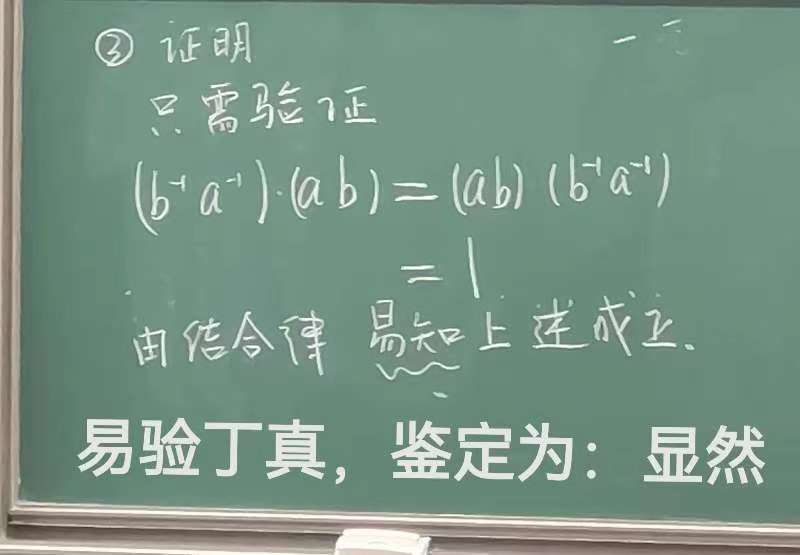
\includegraphics[width=.4\textwidth]{figs/yydz.jpg}
\end{figure}

\end{proof}

\section*{1.\yuedu}

设$A_i,i\in I$是一族非空集合, 定义这些集合的乘积
$\prod_{i\in I}A_i=\{(a_i)_{i\in I}:a_i\in A\}$, 
那么选择公理等价于$\prod_{i\in I}A_i\ne\emptyset$. 

\section*{2.}

考虑$\Z$的模$n$同余等价类集合$\Z_n=\Z/\sim\ =\{\cl{0},\cl{1},\cdots,\cl{n-1}\}$, 
在上面定义乘法$\cl{i}\cdot\cl{j}=\cl{ij}$. 

\subsection*{(1)}

请验证该运算是良定的. 

\begin{proof}
设$\cl{i}=\cl{i'}$, $\cl{j}=\cl{j'}$, 则存在$k_1,k_2\in\Z$
使得$i-i'=k_1n$, $j-j'=k_2n$. 故由
\[ij-i'j'=(i-i')j+i'(j-j')=k_1nj+k_2ni\equiv 0\mod{n}\]
得该运算良定. 
\end{proof}

\subsection*{(2)}

设$(\Z_n)^*=\{\cl{i}:\gcd(i,n)=1\}$, 
证明$(\Z_n)^*$在上述乘法下是一个群. 

\begin{proof}
设$\cl{a},\cl{b}\in(\Z_n)^*$, 则由$\gcd(a,n)=\gcd(b,n)=1$
得$\gcd(ab,n)=1$, 故$\cl{a}\cdot\cl{b}=\cl{ab}\in(\Z_n)^*$. 

结合律: 
由整数乘法结合律即得. 

单位元: 
容易验证$\cl{1}\cdot\cl{a}=\cl{a}\cdot\cl{1}=\cl{a}$. 

逆元: 
$\gcd(a,n)=1$, 由Bezout等式, 存在$s,t\in\Z$使得$as+nt=1$, 
故$as\equiv 1\mod{n}$, 且可得$\gcd(s,n)=1$, 故$\cl{s}\in(\Z_n)^*$. 
\end{proof}

\subsection*{(3)}

记$\varphi(n)=\abs{(\Z_n)^*}$, 称之为{\bf 欧拉函数}. 
设$p$是素数, $m$是正整数, 计算$\varphi(p^m)$, $\varphi(300)$. 

\begin{solution}
小于$p^m$且不与$p^m$互素的自然数只有$0,p,2p,\cdots,(p^{m-1}-1)p$, 
故$\varphi(p^m)=p^m-p^{m-1}$. 

由$\varphi$是积性的, 得$\varphi(300)=\varphi(2^2)\cdot\varphi(3)\cdot\varphi(5^2)
=2\cdot 2\cdot 20=80$. 
\end{solution}

\section*{3.}

记$\GL_n(\Z)$为行列式为$\pm 1$的整系数$n$阶方阵集合. 
验证$\GL_n(\Z)$关于矩阵乘法是一个群. 

\begin{proof}
设$A,B\in\GL_n(\Z)$, 则$\det(AB)=\det A\cdot\det B=\pm 1$.

结合律: 
矩阵乘法有结合律. 

单位元: 
容易验证$I_n\cdot A=A\cdot I_n=A$. 

逆元: 
对任意$A\in\GL_n(\Z)$, 可得$AA^*=A^*A=\det A\cdot I_n$, 
其中$A^*$为$A$的伴随矩阵. 由伴随矩阵定义和整数乘法封闭性可得
$A^*$为整数矩阵. 令$B=A^*/\det A$, 由于$\det A=\pm 1$, 
故$B$也是整数矩阵, 且$AB=BA=I_n$, $\det B=1/\det A=\pm 1$, 
因此$A$有逆元$B\in\GL_n(\Z)$. 
\end{proof}

\begin{remark}
这里有些群友直接由$\det A\ne 0$就得出$A$可逆, 
但这样不能保证$A^{-1}\in\GL_n(\Z)$, 
也就是说不能保证$A$的逆也是整数矩阵. 
\end{remark}

\section*{4.}

设$a$是群$G$中的元素, 约定$a^0=1$. 

\subsection*{(1)}

对于自然数$n$, 证明$(a^n)^{-1}=(a^{-1})^n$. 
后面约定$a^{-n}=(a^{-1})^n$. 

\begin{proof}
只要证$a^n(a^{-1})^n=(a^{-1})^na^n=1$. 这由结合律显然. 
\end{proof}

\subsection*{(2)}

设$k,l\in\Z$, 证明$a^{k+l}=a^k\cdot a^l$. 

\begin{proof}
$k,l\in\N$时由结合律显然. 

$k,l$有一个小于$0$时, 不妨设$k<0$. 若$k+l\ge 0$, 则
$a^{k+l}=1\cdot a^{k+l}=a^{k}\cdot a^{-k}a^{k+l}=a^ka^l$; 
若$k+l<0$, 则$a^{k+l}=(a^{-1})^{-k-l}=(a^{-1})^{-k-l}\cdot 1
=(a^{-1})^{-k-l}(a^{-1})^la^l=(a^{-1})^{-k}a^l=a^ka^l$. 

$k,l<0$时$a^{k+l}=(a^{-1})^{-k-l}=(a^{-1})^{-k}(a^{-1})^{-l}=a^ka^l$. 
\end{proof}

\clearpage
\part{3.13 - 3.19}

\section*{P11-1.2.15.}

对任意$a\in G$, $a\mapsto a^{-1}$是群$G$的自同构当且仅当$G$是交换群. 

\begin{proof}
令$f:G\to G,a\mapsto a^{-1}$.

$\implies$: 
对任意$a,b\in G$, 若$f\in\Aut G$, 则$ab=f(b^{-1}a^{-1})=f(b^{-1})f(a^{-1})=ba$. 

$\impliedby$: 
容易验证$f$是双射. 对任意$a,b\in G$, 有$f(a)f(b)=a^{-1}b^{-1}=(ba)^{-1}=f(ba)=f(ab)$. 
\end{proof}

\section*{P17-1.3.1.}

试证群$G$的任意多个子群的交仍是$G$的子群. 

\begin{proof}
设$A_i\le G$, $i\in I$. 对任意$a,b\in\bigcap_{i\in I}A_i$, 
由每个$A_i\le G$, 得$ab^{-1}\in A_i,\forall i\in I$. 
故$ab^{-1}\in\bigcap_{i\in I}A_i$, 
由\myref[subgroup]{1.3.2.}得$\bigcap_{i\in I}A_i\le G$. 
\end{proof}

\begin{remark}
这里$\bigcap_{i\in I}A_i$不能写成$\bigcap^\infty_{i=1}A_i$, 
更不能写成$\bigcap^n_{i=1}A_i$. 前者意味着可数, 后者意味着有限. 
\end{remark}

\section*{P17-1.3.2.}
\label{subgroup}

设$A$是群$G$的非空子集. 试证$A$是$G$的子群当且仅当对任意
$a,b\in A$有$ab^{-1}\in A$\kh{这也相当于$AA^{-1}=A$}. 

\begin{proof}
$\implies$: 
若$A\le G$, 则对任意$a,b\in A$有$b^{-1}\in A$, 进而有$ab^{-1}\in A$. 

$\impliedby$: 
结合律显然. 
幺元: 对任意$a\in A$, 有$aa^{-1}=1\in A$. 
逆元: 令$a=1$, 则对任意$b\in A$有$b^{-1}\in A$. 
封闭性: 对任意$a,b\in A$, 可知$b^{-1}\in A$, 
故$a(b^{-1})^{-1}=ab\in A$. 
\end{proof}

\section*{P17-1.3.5.\normalsize 重要}

设$A,B$是群$G$的两个子群. 试证: $AB$是$G$的子群当且仅当$AB=BA$. 

\begin{proof}
$\implies$: 对任意$a\in A,b\in B$有$ab\in AB$. 对任意$a\in A,b\in B$, 
由$A,B\le G$有$a^{-1}\in A,b^{-1}\in B$. 对任意$ba\in BA$, 
注意到$ba=(a^{-1}b^{-1})^{-1}$和$a^{-1}b^{-1}\in AB$, 
又由$AB\le G$有$(a^{-1}b^{-1})^{-1}=ba\in AB$, 得$BA\subseteq AB$. 

另一方面, 对任意$ab\in AB$, 由$AB\le G$可知$b^{-1}a^{-1}=
(ab)^{-1}\in AB$, 故存在$a'\in A,b'\in B$使得$b^{-1}a^{-1}=a'b'$. 
同时由$a^{-1}\in A,b^{-1}\in B$可得$a'b'=b^{-1}a^{-1}\in BA$,
故$ab=(b^{-1}a^{-1})^{-1}=b'^{-1}a'^{-1}\in BA$, 得$AB\subseteq BA$. 
因此有$AB=BA$. 

$\impliedby$: 对任意$a_1b_1,a_2b_2\in AB$, 其中$a_1,a_2\in A$, $b_1,b_2\in B$, 
有$a_1b_1(a_2b_2)^{-1}=a_1b_1b_2^{-1}a_2^{-1}\in ABA=AAB=AB$, 
故由\myref[subgroup]{1.3.2.}得$AB\le G$. 
\end{proof}

\begin{remark}
这里我看到有几位群友证得$BA\subseteq AB$后构造了个双射$f:AB\to BA$
或$g:BA\to AB$, 试图以此证明$BA=AB$. 然而对于集合$S_2\subseteq S_1$, 
即使存在双射$f:S_1\to S_2$, 也未必有$S_1=S_2$. 一个反例是$S_1=\Z\supsetneq 2\Z=S_2$, 
可知$f:S_1\to S_2$, $n\mapsto 2n$为双射. 但是如果$S_1\subseteq S_2$是有限集, 
且存在双射$f:S_1\to S_2$, 那么一定有$S_1=S_2$. 
\end{remark}

\section*{P18-1.3.13.}

设$a,b$是群$G$的任意两个元素. 试证: $a$和$a^{-1}$, $ab$和$ba$有相同的阶. 

\begin{proof}
若$\ord(a)<\infty$, 设$\ord(a)=m$. 由$a^m=1$得$(a^{-1})^m=(a^m)^{-1}=1$, 
可知$\ord(a^{-1})\mid m$, 同理$m\mid\ord(a^{-1})$, 
故$\ord(a)=\ord(a^{-1})$. 

若$\ord(a)=\infty$, 假设$\ord(a^{-1})=m'<\infty$, 
则$(a^{m'})^{-1}=(a^{-1})^{m'}=1$, 即$a^{m'}=1$, 矛盾, 得$\ord(a^{-1})=\infty$. 

\vspace{1em}

若$\ord(ab)<\infty$, 设$\ord(ab)=m$, 则由$(ba)^{m+1}=b(ab)^ma=ba$知$(ba)^m=1$, 
得$\ord(ba)\mid m$, 同理$m\mid\ord(a^{-1})$, 故$\ord(ab)=\ord(ba)$. 

若$\ord(ab)=\infty$, 假设$\ord(ba)=m'<\infty$, 
则$(ab)^{m'}=a(ba)^{m'}a^{-1}=a\cdot 1\cdot a^{-1}=1$, 矛盾, 得$\ord(ba)=\infty$. 
\end{proof}

\begin{remark}
这里有不少群友没考虑$\ord(a)=\infty$和$\ord(ab)=\infty$的情况. 
\end{remark}

\section*{1.}
\label{f-with-f(1)}

设$G$是一个群, 取$g\in G$, 则$g$决定了一个群同态
$f_g:\Z\to G$, $i\mapsto g^i$. 反过来, 一个群同态
$f:\Z\to G$由$f(1)$唯一确定. 

\begin{proof}
对任意$i,j\in\Z$,可知$f_g(i+j)=g^{i+j}=g^i\cdot g^j=f(i)\cdot f(j)$, 
故$f_g:\Z\to G$为群同态. 

反过来, 对每个群同态$f:\Z\to G$和任意的$i\in\N$, 
有$f(i)=f(\overbrace{1+\cdots+1}^i)=f(1)^i$, 而$i\in\Z_{<0}$时
$f(i)=f(-i)^{-1}=f(\underbrace{1+\cdots+1}_{-i})^{-1}=f(1)^i$, 
故$f$可由$f(1)$唯一确定. 
\end{proof}

\section*{2.}

利用{\bf 1.}所述结论确定$\Aut(\Z,+)$, 以及用这种思想确定$\Aut(\Q,+)$. 

\begin{solution}
对$f\in\Aut(\Z,+)$, 设$f(1)=a$, 故对任意$b\in\Z$, 有$f(b)=f(1)\cdot b=ab$, 
且$f$为满射, 即存在$b\in\Z$有$ab=1$, 因此$a=\pm 1$. 故$\Aut(\Z,+)=\{b\mapsto ab:a=\pm 1\}=(\Z/2\Z,+)$. 

对$g\in\Aut(\Q,+)$, 设$g(1)=a$, 故对任意$q\in\Z_{>0}$, 有$g(1)=f(\overbrace{1/q+...+1/q}^q)=g(1/q)\cdot a$, 
故$g(1/q)=a/q$. 对任意$p\in\Z$, 与上段类似地有$g(p/q)=g(1/q)\cdot p=ap/q$, 且$a\ne 0$时容易验证$g^{-1}(r)=r/a$. 
故$\Aut(\Q,+)=\{r\mapsto ar:a\in\Q^*\}\isom(\Q^*,\cdot)$. 
\end{solution}

\section*{3.}

在$S_3$中找一个子群$H$使得存在置换$\sigma$满足$\sigma H\ne H\sigma$. 

\begin{solution}
\kh{不唯一; 这个我懒得算了, 参考一下某位群友的作业} 
注意到$(12)(123)=(13)$, $(123)(12)=(23)$. 令$H=\{1,(12)\}$, 
$\sigma=(123)$, 则$\sigma H=\{(123),(23)\}\ne\{(123),(13)\}=H\sigma$. 
\end{solution}

\section*{4.}
\label{GL-SL}

考虑子群$\SL(n,\R)\le\GL(n,\R)$. 证明: 两个矩阵属于
$\SL(n,\R)$的同一个左陪集当且仅当它们的行列式相等. 

\begin{proof}
$\implies$: 
设$A,B\in\GL(n,\R)$属于$\SL(n,\R)$的同一个左陪集$A\cdot\SL(n,\R)$, 
则存在$C\in\SL(n,\R)$使得$B=AC$, 故$\det B=\det A\cdot\det C=\det A\cdot 1=\det A$. 

$\impliedby$: 
设$A,B\in\GL(n,\R)$满足$\det A=\det B\ne 0$, 则有$\det A^{-1}B=\det A^{-1}\cdot\det B=1$, 
即$A^{-1}B\in\SL(n,\R)$, 故$B=AA^{-1}B\in A\cdot\SL(n,\R)$, 
即$A,B$属于$\SL(n,\R)$的同一个左陪集. 

令$\F$为$\SL(n,\R)$的所有左陪集, $f:\mathcal{F}\to\R^*,A\cdot\SL(n,\R)\mapsto\det A$. 
由上述证明可知$f$是良定的, 且为$\mathcal{F}$与$\R^*$之间的双射. 
\end{proof}

\section*{5.\normalsize 重要}

设群$G$中的元素$a,b$的阶分别为$m,n$, 如果$ab=ba$
且$\gcd(m,n)=1$. 

\subsection*{(1)}

证明对任意$i,j\in\Z$有$a^ib^j=b^ja^i$\kh{因为非常显然, 不怀疑的话不用证}. 

\begin{proof}
不妨设$0\le i\le m-1$, $0\le j\le n-1$, 这样就显然了. 
\end{proof}

\subsection*{(2)}

课上已经证明过$\gen{a}=\{1,a,\cdots,a^{m-1}\}$是$G$的子群, 
请证明$\gen{a}\cap\gen{b}=\{1\}$. 

\begin{proof}
若$\gen{a}\cap\gen{b}\ne\{1\}$, 
由$\gen{a}\cap\gen{b}\le\gen{a}$
也是循环群, 得$\gen{a}\cap\gen{b}$有生成元$c\ne 1$. 
设$\ord(c)=u>1$, 则可知$u\mid m$, $u\mid n$, 这与$\gcd(m,n)=1$矛盾. 
\end{proof}

\subsection*{(3)}
\label{ord-mul}

$\ord(ab)=mn$. 

\begin{proof}
对任意的$s\in\{1,...,m-1\}$, $t\in\{1,...,n-1\}$, 假如$a^sb^t=1$, 
则$a^s=b^{-t}=b^{n-t}$, 且$n-t\in\{1,...,n-1\}$, 由(2)得此时只能有$a^s=b^{n-t}=1$, 
这与$\ord(a)=m$, $\ord(b)=n$矛盾, 故总有$a^sb^t\ne 1$, 进而可以得到
$a^sb^t=1$当且仅当$m\mid s$, $n\mid t$. 对$d\in\Z$, 若$(ab)^d=a^db^d=1$, 
则有$m\mid d$, $n\mid d$, 故$mn=\lcm(m,n)\mid d$. 又$(ab)^{mn}=a^{mn}b^{mn}=1$, 得$\ord(ab)=mn$. 
\end{proof}

\section*{6.\normalsize 如果觉得显然就阅读}

设$A,B,C$是群$G$的非空子集, 定义
$A\cdot B=\{a\cdot b:a\in A,\ b\in B\}$和
$A^{-1}=\{a^{-1}:a\in A\}$. 
验证: $(AB)C=A(BC)$, $(AB)^{-1}=B^{-1}A^{-1}$, 
$gA=gB\iff A=B$, 以及$gA=B\iff A=g^{-1}B$. 

\begin{proof}
直接按定义验证即可. 
\end{proof}

\section*{7.}

设$A\le G$, 证明作为集合有$(gA)^{-1}=Ag^{-1}$, 
以此可以直接证明左右陪集一一对应. 

\begin{proof}
\kh{这个上课是不是也证过}一方面, 对任意$x=(ga)^{-1}\in(gA)^{-1}$, 
由$x=a^{-1}g^{-1}$和$a^{-1}\in A$得$x\in Ag^{-1}$, 故$(gA)^{-1}\subseteq Ag^{-1}$; 
另一方面, 对任意$y=ag^{-1}\in Ag^{-1}$, 由$x=(ga^{-1})^{-1}$和
$a^{-1}\in A$得$x\in(gA)^{-1}$, 故$Ag^{-1}\subseteq(gA)^{-1}$. 
因此$(gA)^{-1}=Ag^{-1}$. 
\end{proof}

\section*{8.\xuan}

设$G$为有限群, $A,B$为$G$的子群, 课上已经证明了$C=A\cap B$
也是子群, 设$[A:C]=k$, 记$\{a_1C,\cdots,a_kC\}$为$C$在$A$
中的所有左陪集. 请证明: 

\subsection*{(1)}

对于$i\ne j$, 左陪集$a_iB\ne a_jB$. 

\begin{proof}
对于$i\ne j$, 可知$a_iC\ne a_jC$, 即$a_i^{-1}a_j\notin C=A\cap B$. 
由$a_i,a_j\in A\le G$得$a_i^{-1}a_j\in A$, 故$a_i^{-1}a_j\notin B$, 
即$a_iB\ne a_jB$. 
\end{proof}

\subsection*{(2)}

对于任意$a\in A$, 存在$i\in\{1,2,\cdots,k\}$使得$aB=a_iB$. 

\begin{proof}
对于任意$a\in A$, 由于$C\le A$且$C$在$A$中的所有左陪集为$a_1C,...,a_kC$, 
得存在$i$有$aC=a_iC$, 故$a^{-1}a_i\in C\le B$, 得$aB=a_iB$. 
\end{proof}

\subsection*{(3)}

由{\bf (1)(2)}可得$A\cdot B=\bigsqcup^k_{i=1}a_iB$, 
从而$\abs{A\cdot B}=\abs{A}\cdot\abs{B}/\abs{A\cap B}$. 

\begin{proof}
由{\bf (1)(2)}可得$A\cdot B=\bigsqcup^k_{i=1}a_iB$, 故$\abs{AB}=k\cdot\abs{B}=\abs{B}\cdot\abs{A}/\abs{A\cap B}$. 
\end{proof}

\subsection*{(4)}

用类似的办法处理{\bf P18-1.3.11.}: 设$H$和$K$分别是有限群$G$的两个子群, 
试证$\abs{HgK}=\abs{H}\cdot[K:g^{-1}Hg\cap K]$. 

\begin{proof}
容易验证$\abs{HgK}=\abs{g^{-1}HgK}$, $g^{-1}Hg\le G$且$\abs{g^{-1}Hg}=\abs{H}$. 
因此\[\abs{HgK}=\abs{g^{-1}HgK}=\frac{\abs{g^{-1}Hg}\cdot\abs{K}}{\abs{g^{-1}Hg\cap K}}=\abs{H}\cdot[K:g^{-1}Hg\cap K].\]
\end{proof}

\begin{remark}
这里我看到有几位群友对$H$和$gK$应用{\bf (3)}的结论得出
$\abs{HgK}=\abs{H}\cdot\abs{gK}/\abs{H\cap gK}$, 
但$gK$未必是$G$的子群, 所以不能直接用{\bf (3)}. 
\end{remark}

\section*{9.}

设$G$是一个群, 满足对于所有的元素$a$有$a^2=1$. 
证明群$G$是交换群. 

\begin{proof}
可知对任意$a\in G$都有$a^{-1}=a$. 因此对任意$a,b\in G$有
$ab=(ab)^{-1}=b^{-1}a^{-1}=ba$, 故$G$为交换群. 
\end{proof}

\clearpage
\part{3.20 - 3.26}

\section*{P20-1.4.2.}

证明: 群$G$没有非平凡子群的充分必要条件是$G=\{1\}$
或$G$是素数阶循环群. 

\begin{proof}
$\implies$: 
首先$\{1\}$没有非平凡子群. 其次, 若$G\ne\{1\}$则存在$g\in G\setminus\{1\}$. 
当$\abs{G}=\infty$时, 若$\ord(g)<\infty$则$\gen{g}<G$, 若$\ord(g)=\infty$
则$\gen{g^2}<\gen{g}\le G$, 矛盾. 当$\abs{G}<\infty$时对每个$g\in G\setminus\{1\}$
都有$\gen{g}=G$, 得$G$为循环群. 假设$\abs{G}=ab$为合数 (其中$a,b\in\N_+$), 
则由$(g^a)^b=1$可知$\gen{g^a}<G$, 矛盾, 故只能有$G$为素数阶循环群. 

$\impliedby$: 
$\{1\}$没有非平凡子群. 假设素数$p$阶循环群$G$有子群$H\le G$, 
则由$\abs{H}\mid p=\abs{G}$得$\abs{H}=1$或$p$, 都是$G$的平凡子群. 
\end{proof}

\section*{P20-1.4.4.}

设$a$和$b$是群$G$的元素, 阶数分别是$n$和$m$, 
$\gcd(n,m)=1$且$ab=ba$. 试证$\gen{ab}$是$G$的$mn$阶循环子群. 

\begin{proof}
同\myref[ord-mul]{第2周5.(3)}. 
\end{proof}

\section*{P20-1.4.6.}

设$G$是一个$n$阶有限群, 若对$n$的每一因子$m$, 
$G$中至多只有一个$m$阶子群, 则$G$是循环群. 

\begin{proof}
先证明对$n$的每个正因子$m$, $G$中阶为$m$的元素至多有$\varphi(m)$个. 
假如有超过$\varphi(m)$个, 设其中一个为$a$, 则$\gen{a}<G$, 
$\gen{a}$中阶为$m$的元素有$\varphi(m)$个, 故存在阶为$m$的$b\in G\setminus\gen{a}$, 
得$G$有至少两个$m$阶子群$\gen{a},\gen{b}$, 矛盾. 

设$G$中阶为$m$的元素有$f(m)$个, 则$f(m)\le\varphi(m)$. 由
$n=\sum_{m\mid n}f(m)\le\sum_{m\mid n}\varphi(m)=n$
得$f(m)=\varphi(m)$, 特别地有$f(n)=\varphi(n)\ge 1$, 
即$G$中存在$n$阶元, 故为循环群. 
\end{proof}

\begin{remark}
可以用这个命题证明有限域的单位群$(\F_{p^n})^*$为循环群. 
\end{remark}

\section*{P25-1.5.2.}

设$G$是群, $N<M<G$. 

\subsection*{(1)}

如果$N\lhd G$, 则$N\lhd M$. 

\begin{proof}
由$N\lhd G$, 得对任意$g\in G$有$gNg^{-1}=N$, 
故对任意$g\in M<G$有$gNg^{-1}=N$, 又$N<M$, 得$N\lhd M$. 
\end{proof}

\subsection*{(2)}

如果$N\lhd M$, 那$N$是否一定是$G$的正规子群? 

\begin{solution}
不一定. 以下给出群友们的智慧: 

\begin{itemize}[itemsep=0em]
    \item $\Z_2\lhd K_4\lhd A_4$, 但$\Z_2\nlhd A_4$. 
    \item $N$为所有对角元为$1$的$n$阶上三角实方阵, $M$为所有对角元非零的$n$阶上三角实方阵, $G=\text{GL}_n(\R)$, 则$N\lhd M<G$, 但$N\nlhd G$. 
    \item 自由群$\gen{a^2}\lhd\gen{a}<\gen{a,b}$, 但$\gen{a^2}\nlhd\gen{a,b}$. 
\end{itemize}
\end{solution}

\section*{P25-1.5.4.}

试证群$G$的指数为$2$的子群一定是$G$的正规子群. 

\begin{proof}
设$H\lhd G$, $[G:H]=2$. 对任意$g\in G\setminus H$, 则$G=H\sqcup gH=H\sqcup Hg$, 
故$gH=Hg=G\setminus H$, 即$gHg^{-1}=H$; 而对任意$g\in H$有$gH=Hg=H$, 也有$gHg^{-1}=H$. 
因此$H\lhd G$. 
\end{proof}

\section*{P25-1.5.7.}

设$M$和$N$分别是群$G$的正规子群. 如果$M\cap N=\{1\}$, 
则对任意$a\in M$, $b\in N$, 都有$ab=ba$. 

\begin{proof}
只要证$ab(ba)^{-1}=aba^{-1}b^{-1}=1$. 注意到$aba^{-1}\in aNa^{-1}=N$
且$b^{-1}\in N$, 有$aba^{-1}\cdot b^{-1}\in N$; 又$ba^{-1}b^{-1}\in bMb^{-1}=M$
且$a\in M$, 有$a\cdot ba^{-1}b^{-1}\in M$, 故$aba^{-1}b^{-1}\in M\cap N=\{1\}$. 
\end{proof}

\section*{1.}

设$G$是有限群, 假设存在元素$a$使得$G=\gen{a}$, 
此时称$G$为{\bf 循环群}, $a$称作$G$的一个{\bf 生成元}. 

\subsection*{(1)}

群同态$f:G\to K$由$f(a)$唯一确定. 

\begin{proof}
与\myref[f-with-f(1)]{第2周1.}证明$f:\Z\to K$由$f(1)$唯一确定的思路类似. 
\end{proof}

\subsection*{(2)}

如果$f:\Z_{12}\to\Z_{16}$是一个群同态, 设$f(\cl{1})=\cl{k}\in\Z_{16}$, 
问$\cl{k}$可以取哪些值? 

\begin{solution}
群同态$f:\Z_{12}\to\Z_{16}$由$f(\cl{1})=\cl{k}$唯一确定, 由$12\cdot\cl{k}=f(12\cdot\cl{1})=f(\cl{0})=\cl{0}$
得$\ord(\cl{k})\mid 12$, 又$\ord(\cl{k})\mid 16$, 得$\ord(\cl{k})\mid\gcd(12,16)=4$, 
故$\cl{k}\in\{\cl{0},\cl{4},\cl{8},\cl{12}\}$. 
\end{solution}

\section*{2.\xuan}

证明: $\Aut\Z_n\isom(\Z_n)^*$\kh{注意证明群同构, 不仅仅一一对应}. 

\begin{proof}
$f\in\Aut\Z_n$由$f(\cl{1})$唯一确定, 记$f_{\cl{a}}$为满足$f(\cl{1})=\cl{a}$的自同构$f$. 

由于$f_{\cl{a}}$为自同构, 故$\ord(\cl{a})=\ord(\cl{1})=n$. 设$\gcd(n,a)=d$, 
则由$n\mid n/d\cdot a$得$n/d\cdot\cl{a}=\cl{0}$, 故$\ord(\cl{a})\mid n/d$, 
因此有$d=1$, 即$\cl{a}\in(\Z_n)^*$. 反过来, 每个$\cl{a}\in(\Z_n)^*$
决定一个$f_{\cl{a}}:\cl{1}\mapsto\cl{a}$. 

令$g:(\Z_n)^*\to\Aut\Z_n,\cl{a}\mapsto f_{\cl{a}}$, 则$g$为双射. 
注意到$f_{\cl{a}}\circ f_{\cl{b}}(1)=f_{\cl{a}}(\cl{b})=\cl{b}\cdot f_{\cl{a}}(\cl{1})=\cl{b}\cdot\cl{a}=\cl{ab}$, 
可得$f_{\cl{a}}\circ f_{\cl{b}}=f_{\cl{ab}}$, 即$g(a)g(b)=g(ab)$, 得$g$为同构. 
\end{proof}

\section*{3.}

证明: $\gen{\cl{22},\cl{55}}=\Z_{100}$. 

\begin{proof}
显然$\gen{\cl{22},\cl{55}}\le\Z_{100}$. 由$\cl{11}=\cl{55}-2\cdot\cl{22}$
和$\gcd(11,100)=1$, 得$\cl{11}$是$\Z_{100}$的生成元, 
故$\gen{\cl{22},\cl{55}}\ge\gen{\cl{11}}=\Z_{100}$. 
因此有$\gen{\cl{22},\cl{55}}=\Z_{100}$. 
\end{proof}

\section*{4.}

设$N$是$G$的正规子群, 验证$aN\cdot bN=abN$\kh{集合乘积}. 

\begin{proof}
由$N\lhd G$得$bN=Nb$, 故$aN\cdot bN=a\cdot Nb\cdot N=a\cdot bN\cdot N=abN$. 
\end{proof}

\section*{5.}

描述$\Z_{12}$到$\Z_{20}$的所有群同态. 

\begin{solution}
群同态$f:\Z_{12}\to\Z_{20}$由$f(\cl{1})=\cl{k}$唯一确定, 
由$12\cdot\cl{k}=f(12\cdot\cl{1})=f(\cl{0})=\cl{0}$得$\ord(\cl{k})\mid 12$, 
又$\ord(\cl{k})\mid 20$, 得$\ord(\cl{k})\mid\gcd(12,20)=4$, 
故$\cl{k}\in\{\cl{0},\cl{5},\cl{10},\cl{15}\}$, 
即$\Z_{12}$到$\Z_{20}$的所有群同态为$\{f_{\cl{0}},f_{\cl{5}},f_{\cl{10}},f_{\cl{15}}\}$. 
\end{solution}

\section*{6.}

设$A$是群$G$的非空子集. 

\subsection*{(1)}

证明集合$N_G(A)=\{g\in G:g^{-1}Ag=A\}$是一个子群, 称作$A$的{\bf 正规化子群}. 

\begin{proof}
$1\in N_G(A)\ne\emptyset$. 对任意$g,h\in N_G(A)$, 有
$g^{-1}hAh^{-1}g=g^{-1}h\cdot h^{-1}Ah\cdot h^{-1}g=g^{-1}Ag=A$, 
故$gh^{-1}\in N_G(A)$, 得$N_G(A)\le G$. 
\end{proof}

\subsection*{(2)}

证明集合$C_G(A)=\{g\in G:ga=ag,\forall a\in A\}$是一个子群, 
称作$A$的{\bf 中心化子群}. 

\begin{proof}
$1\in C_G(A)\ne\emptyset$. 由$ga=ag$得$g^{-1}ag=gag^{-1}=a$. 
对任意$g,h\in C_G(A)$, 有$gh^{-1}ahg^{-1}=gag^{-1}=a$, 
即$gh^{-1}a=agh^{-1}$, 故$gh^{-1}\in C_G(A)$, 得$C_G(A)\le G$. 
\end{proof}

\subsection*{(3)}

当$A=G$时, 子群$C_G(G)$通常记作$C(G)$, 称作$G$的{\bf 中心}, 
证明$C(G)$是$G$的正规子群. 

\begin{proof}
对任意$x\in C(G)$和任意$g\in G$有$gxg^{-1}=x$, 
故$gC(G)g^{-1}=\{gxg^{-1}:x\in C(G)\}=C(G)$, 
得$C(G)\lhd G$. 
\end{proof}

\subsection*{(4)\xuan}

证明: 如果$G/C(G)$是循环群, 那么$G$是交换群. 

\begin{proof}
设$G/C(G)=\gen{a}$, 则对任意$g,h\in G$, 
存在$x,y\in C(G)$和$m,n\in\Z$有$g=a^mx,h=a^ny$. 
因此有$gh=a^mxa^ny=a^ma^nxy=a^na^myx=a^nya^mx=hg$, 
得$G$为交换群. 
\end{proof}

\section*{7.}

证明群同构$\GL_n(\R)/\SL_n(\R)\isom\R^*$. 

\begin{proof}
设$f:\GL_n(\R)\to\R^*$, $A\mapsto\det A$. 
由$f(AB)=\det AB=\det A\cdot\det B=f(A)f(B)$得$f$为群同态. 
对任意$a\in\R^*$, 由$f(\mathrm{diag}(a,1,...,1))=a$, 得$\im f=\R^*$. 
又$\ker f=f^{-1}(1)=\SL_n(\R)$, 故由同态基本定理得
$\GL_n(\R)/\SL_n(\R)\isom\im f=\R^*$. 
\end{proof}

布置这个题的时候还没学同态基本定理, 这里再给出一种直接把陪集映射到行列式的做法. 

\begin{proof}
设$g:\GL_n(\R)/\SL_n(\R)\to\R^*$, $\cl{A}=A\cdot\SL_n(\R)\mapsto\det A$. 
\myref[GL-SL]{第2周4.}已证得$g$为良定的双射. 又$g(\cl{A})\cdot g(\cl{B})=
\det A\cdot\det B=\det AB=g(\cl{AB})$, 得$g$为同构. 
\end{proof}

\clearpage
\part{3.27 - 4.2}

\section*{P25-1.5.6.}

设$f:G\to H$是群同态, $M\le G$, 试证$f^{-1}(f(M))=KM$, 这里$K=\ker f$. 

\begin{proof}
对任意$x\in f^{-1}(f(M))$, 有$f(x)\in f(M)$, 故存在$m\in M$有
$f(x)=f(m)$. 因此有$f(xm^{-1})=f(x)\cdot f(m)^{-1}=1$, 得$xm^{-1}\in\ker f=K$, 
故$x=xm^{-1}\cdot m\in KM$. 因此$f^{-1}(f(M))\subseteq KM$. 
对任意$x\in KM$, 存在$k\in K$和$m\in M$有$x=km$, 故
$f(x)=f(k)f(m)=f(m)\in f(M)$. 因此$f^{-1}(f(M))\supseteq KM$. 
综上, 有$f^{-1}(f(M))=KM$. 
\end{proof}

\begin{remark}
这里有的群友试图通过证明$f(M)=f(KM)$来证得结论, 但这与待证命题不等价. 
容易注意到$f(M)=f(M)$, 但$K$不是$M$的子群时$f^{-1}(f(M))\ne M$. 
$f^{-1}(f(M))$是集合$f(M)$中元素\yh{所有}原像组成的集合, 要证明的是
\yh{所有}原像正好是集合$KM$. 
\end{remark}

\section*{P25-1.5.8.}

设$f:G\to H$是群同态. 如果$g$是$G$的一个有限阶元素, 则$f(g)$的阶整除$g$的阶. 

\begin{proof}
设$\ord(g)=n$, 则$g(n)=1$, 故$f(g)^n=f(g^n)=f(1)=1$, 得$\ord(f(g))\mid n=\ord(g)$. 
\end{proof}

\section*{P25-1.5.9.}

设$N\lhd G$, $g$是群$G$的任意一个元素. 如果$g$的阶和$\abs{G/N}$
互素, 则$g\in N$. 

\begin{proof}
设$\ord(g)=n$, 则$\cl{g}^n=\cl{g^n}=\cl{1}$, 
得$\ord(\cl{g})\mid n$. 又$\abs{G/N}<\infty$, 得
$\ord(\cl{g})\mid\abs{G/N}$. 因此$\ord(\cl{g})\mid\gcd(n,\abs{G/N})=1$, 
得$\cl{g}=\cl{1}$, 即$g\in N$. 
\end{proof}

\section*{P30-1.6.1.}

把置换$\sigma=(456)(567)(761)$写成不相交轮换的积. 

\begin{solution}
\sout{偷懒}方便起见, $2$和$3$省略. 
\[(1,4,5,6,7)\rto{(761)}(7,4,5,1,6)\rto{(567)}(5,4,6,1,7)\rto{(456)}(6,5,4,1,7)\]
可见$\sigma=(16)(45)$. 
\end{solution}

\section*{P30-1.6.2.}

讨论置换$\sigma=\pmat{1&2&\cdots&n\\n&n-1&\cdots&1}$的奇偶性. 

\begin{solution}
注意到$\sigma=(1n)(2,n-1)\cdots(\floor{n/2},n+1-\floor{n/2})$, 
为$\floor{n/2}$个对换之积, 
故$\sigma$的奇偶性与$\floor{n/2}$奇偶性相同, 
即$n\equiv 0,1\mod{4}$时$\sigma$为奇置换, 
$n\equiv 2,3\mod{4}$时$\sigma$为偶置换. 
\end{solution}

\begin{remark}
如果还记得线性代数讲行列式时讲过的\yh{逆序数}, 
可以发现$\sigma$的每一对都是逆序对, $\sigma$的逆序数为
$\mathrm{C}^2_n=\frac12n(n-1)$, 故$\sigma$的奇偶性与
$\frac12n(n-1)$的奇偶性相同, 即$n\equiv 0,1\mod{4}$时
$\sigma$为奇置换, $n\equiv 2,3\mod{4}$时$\sigma$为偶置换. 
\end{remark}

\section*{P30-1.6.4.}

设$\sigma=(12\cdots n)$为$S_n$的一个全轮换, 
试证$C_{S_n}(\sigma)=\gen{\sigma}$. 

\begin{proof}
对任意$\tau\in\gen{\sigma}$, 设$\tau=\sigma^i$, 
则$\tau\sigma=\sigma^{i+1}=\sigma\tau$, 
故$\gen{\sigma}\subseteq C_{S_n}(\sigma)$. 
对任意$\tau\in C_{S_n}(\sigma)$和任意$j\in\Z_n$, 
可知$\tau(j+1)=\tau\sigma(j)=\sigma\tau(j)
=\tau(j)+1\mod{n}$. 设$\tau(1)=k$, 则递推可知
$\tau(j)=k+j-1\mod{n}$, 得$\tau=\sigma^{k-1}\in\gen{\sigma}$. 
综上, 有$C_{S_n}(\sigma)=\gen{\sigma}$. 
\end{proof}

还有一位群友给出了这样的做法. 

\begin{proof}
对任意$\tau\in\gen{\sigma}$, 设$\tau=\sigma^i$, 
则$\tau\sigma=\sigma^{i+1}=\sigma\tau$, 
故$\gen{\sigma}\subseteq C_{S_n}(\sigma)$. 
$\sigma$所在的共轭类$C_\sigma$
为所有$n^1$型置换的集合, 故$\abs{C_\sigma}=(n-1)!$. 
由$\abs{C_\sigma}\cdot\abs{C_G(\sigma)}=\abs{S_n}=n!$, 
得$\abs{C_{S_n}(\sigma)}=n$. 又$\abs{\gen{\sigma}}=n$, 
$\gen{\sigma}\subseteq C_{S_n}(\sigma)$, 
得$C_{S_n}(\sigma)=\gen{\sigma}$. 
\end{proof}

\begin{remark}
对任意群$G$和$g\in G$, 有$\abs{C_g}=[G:C_G(g)]$. 证明在书上P16. {\rm\cite{jsds}}
\end{remark}

\section*{P30-1.6.5.}

试证一个置换的阶等于它的轮换表示中各个轮换的长度的最小公倍数. 

\begin{proof}
设$\sigma_1,\cdots,\sigma_k$为不相交轮换, 长度分别为$n_1,\cdots,n_k$, 
则易知$\ord(\sigma_i)=n_i$. 令$\tau=\sigma_1\cdots\sigma_k$. 
由于这些$\sigma_i$不相交, 可知其中任意两个可交换, 
故由$\tau^m=\sigma_1^m\cdots\sigma_k^m=1$得
对每个$i$都有$\sigma_i^m=1$, 故$n_i\mid m$, 
因此$\lcm(n_1,\cdots,n_k)\mid m$. 又$m=\lcm(n_1,\cdots,n_k)$
时即有$\tau^m=1$, 故$\ord(\tau)=\lcm(n_1,\cdots,n_k)$. 
\end{proof}

\section*{P30-1.6.6.}

试确定$S_4$的全部正规子群. 

\begin{solution}
$S_4$有两个平凡正规子群$\{1\}$和$S_4$. 可知$S_4$的非平凡正规子群$H$
是一些共轭类之并, 而且只可能是$2,3,4,6,8,12$阶. 先对$S_4$中的元素按
共轭类分类, 即按型分类: 
\begin{itemize}[itemsep=0pt]
    \item $1^1$型: $1$个
    \item $2^1$型: $\mathrm{C}^2_4=6$个
    \item $2^2$型: $\mathrm{C}^2_4/2=3$个
    \item $3^1$型: $\mathrm{C}^3_4\cdot(3-1)!=8$个
    \item $4^1$型: $(4-1)!=6$个
\end{itemize}

$S_4$的子群一定包含$1$, 因此只可能有$\abs{H}=4=1+3$
或$\abs{H}=12=1+3+8$. $\abs{H}=4$时$H$只包含$1$和
所有$2^2$型置换, 故$H=\{1,(12)(34),
(13)(24),(14)(23)\}$, 容易验证此时$H\isom K_4$; 
$\abs{H}=12$时$H$只包含$1$, 所有$2^2$型和所有$3^1$型置换, 
即包含所有偶置换, 此时$H=A_4$. 
因此$S_4$的所有正规子群有$\{1\},K_4,A_4,S_4$. 
\end{solution}

\begin{remark}
\myref[A4-lhd]{第4周习题课讲义1.}\yh{求$A_4$全部正规子群}的方法可以照葫芦画瓢
用在这个题上, 但上段所述方法用于求$A_4$正规子群时要谨慎. 对$A_n$中
的元素按共轭类分类时不能简单地按型分类, 
如$(123)$和$(132)$在$S_4$中是共轭的, 但在$A_4$中不是. 
\end{remark}

证明$(123),(132)\in A_4$不共轭: 

\begin{proof}
假设存在$\sigma\in A_4$
有$\sigma(123)\sigma^{-1}=(\sigma(1)\sigma(2)\sigma(3))=(132)=(321)=(213)$, 
可知$\{1,2,3\}$中必有一个是$\sigma$的不动点, 而另外两个被$\sigma$对换. 
比如设$1$为$\sigma$的不动点, 则$\sigma=(23)$. 这样的$\sigma$是奇置换, 
与$\sigma\in A_4$矛盾. 
\end{proof}

\begin{remark}
这也说明了型相同的\kh{在$S_n$中是共轭的}置换为什么在$A_n$中未必共轭. 
\end{remark}

\section*{1.}

设$G=\R\times\R$, $H=\R\cdot(1,1)\le G$. 证明: $G/H\isom\R$. 

\begin{proof}
令$f:G\to\R,(x,y)\mapsto x-y$, 则容易验证$f$为群满同态, 
且$\ker f=\{(x,x):x\in\R\}=H$. 故$G/H\isom\im f=\R$.
\end{proof}

\section*{2.}
\label{C-exp}

证明: $(\C/\Z,+)\isom(\C^*,\cdot)$.

\begin{proof}
令$f:\C\to\C^*$, $z\mapsto e^{2\pi iz}$. 
可知$f(z_1+z_2)=e^{2\pi i(z_1+z_2)}=e^{2\pi iz_1}e^{2\pi iz_2}=f(z_1)f(z_2)$, 
故$f$为群同态. 注意到
\[f^{-1}(w)=\left\{\frac{\ln\abs{w}+i\cdot(\arg w+2k\pi)}{2\pi i}:k\in\Z\right\}=\left\{k+\frac{\arg w}{2\pi}-i\cdot\frac{\ln|w|}{2\pi}:k\in\Z\right\},\] 
可知$\im f=\C^*$, $\ker f=f^{-1}(1)=\Z$. 故有
$\C/\Z=\C/\ker f\isom\im f=\C^*$. 
\end{proof}

\section*{3.}

设$\varphi:G\to G'$是满同态, 那么$\varphi$把正规子群映到正规子群. 

\begin{proof}
设$H\lhd G$, $H'=\varphi(H)$, 则对任意$g\in G$有$gHg^{-1}=H$. 
对任意$g'\in G'$, 由$\varphi$为满同态, 存在$g\in G$使得$\varphi(g)=g'$. 故由
$g'H'g'^{-1}=\varphi(g)\varphi(H)\varphi(g)^{-1}
=\varphi(gHg^{-1})=\varphi(H)=H'$得$H'\lhd G'$. 
\end{proof}

\section*{4.}
\label{group-correspond}

设$N\lhd G$, 那么群$G$中包含$N$的\kh{正规}子群和$G/N$的\kh{正规}子群一一对应. 

\begin{proof}
令$p:G\to G/N,g\mapsto gN$, 则$p$为群满同态. 
设$\mathcal{A}=\{M:N\subseteq M\le G\}$为$G$的所有包含$N$的子群, 
$\mathcal{B}=\{M':M'\le G/N\}$为$G/N$的所有子群. 咱们要证明
$u:M\mapsto p(M)$为$\mathcal{A}\to\mathcal{B}$的双射. 

\vspace{1em}

设$M$为$G$的包含$N$的子群, 先证明$\im u\subseteq\mathcal{B}$, 
即证明$M/N\le G/N$. 
由$M\le G$, 令$p'=p|_M:M\to G/N$, 则$p'$也为群同态, 故
$M/N=\{xN:x\in M\}=\im p'\le G/N$. 
为节省篇幅, 以下的$M/N$也写为$\cl{M}$. 

设$M_1\ne M_2$为$G$的两个包含$N$的子群, 然后证明$\cl{M_1}\ne\cl{M_2}$. 
可知存在$x\in M_1\triangle M_2$, 不妨设$x\in M_1\setminus M_2$, 
则$p(x)=xN\in\cl{M_1}$. 假如$xN\in\cl{M_2}$, 由$\cl{M_2}\le\cl{G}$, 
得存在$yN\in\cl{M_2}$使得$xN\cdot yN=xyN=1\cdot N$, 即$xy\in N\le M_2\le G$. 
这样$x=y^{-1}\in M_2$, 与$x\in M_1\setminus M_2$矛盾. 
因此$xN\in\cl{M_1}\setminus\cl{M_2}$, 即$\cl{M_1}\ne\cl{M_2}$. 
至此, 咱们证明了$u:\mathcal{A}\to\mathcal{B}$为单射. 

最后证明$u$为满射, 即证对任意$M'\le G/N$有$p^{-1}(M')\le G$. 
结合律显然. 由$p(1)=\cl{1}\in M'$得$1\in p^{-1}(M')$. 
对任意$a,b\in p^{-1}(M')$, 即$aN,bN\in M'$, 有$aN\cdot bN=abN\in M'$, 
故$ab\in p^{-1}(M')$. 对任意$a\in p^{-1}(M')$, 有$aN\in M'$, 
存在$bN\in M'$使得$abN=aN\cdot bN=\cl{1}=1\cdot N$, 即$ab\in N\lhd G$, 
故存在$c\in N$有$abc=1$, 即$a^{-1}=bc$. 又由$bN\in M'$得
$b\in p^{-1}(M')$, 由$c\in N=p^{-1}(\cl{1})\subseteq p^{-1}(M')$
得$a^{-1}=bc\in p^{-1}(M')$. 因此$p^{-1}(M')\le G$, 得$u$为满射. 

这样就得到$u:\mathcal{A}\to\mathcal{B},M\mapsto p(M)=M/N$为双射\kh{一一对应}. 

\vspace{1em}
令$\mathcal{A}'=\{M\in\mathcal{A}:M\lhd G\}$为$G$的所有包含$N$的正规子群, 
$\mathcal{B}'=\{M'\in\mathcal{B}:M'\lhd G/N\}$为$G/N$的所有正规子群. 
还要证明$u'=u|_{\mathcal{A}'}:\mathcal{A}'\to\mathcal{B}$
为$\mathcal{A}'\to\mathcal{B}'$的双射. 

\vspace{1em}

设$M$为$G$的包含$N$的正规子群, 先证明$\im u'\subseteq\mathcal{B}'$, 
即证$M/N\lhd G/N$. 对任意$g\in G$有$gMg^{-1}=M$, 
又$p$为满同态, 得$p(g)p(M)p(g^{-1})=p(M)$, 即对任意$gN\in G/N$
有$gN\cdot M/N\cdot(gN)^{-1}=M/N$, 
得$M/N\lhd G/N$, 即$\im u'\subseteq\mathcal{B}'$. 

然后证明$u'$为满射, 即证对任意$M'\lhd G/N$有$p^{-1}(M')\lhd G$. 
已证得$p^{-1}(M')\le G$. 对任意$g\in G$, 由$M'\lhd G/N$和$p$为满同态, 可知
$p(gp^{-1}(M')g^{-1})=p(g)p(p^{-1}(M'))p(g^{-1})=gN\cdot M'\cdot(gN)^{-1}=M'$, 
故$gp^{-1}(M')g^{-1}\subseteq p^{-1}(M')$. 同理
$g^{-1}p^{-1}(M')g\subseteq p^{-1}(M')$, 故$p^{-1}(M')\subseteq gp^{-1}(M')g^{-1}$. 
因此$gp^{-1}(M')g^{-1}=p^{-1}(M')$, 得$p^{-1}(M')\lhd G$, 故$u'$为满射. 

由$u$为单射显然有$u'=u|_{\mathcal{A}'}$为单射. 这样也得到
$u':\mathcal{A}'\to\mathcal{B}',M\mapsto p(M)=M/N$为双射\kh{一一对应}. 
\end{proof}

\section*{5.}

设$K$是$G$的指数为$2$的子群, $N\le G$, $N$不是$K$的子群, 
那么$[N:N\cap K]=2$. 

\begin{proof}
由$[G:K]=2$有$K\lhd G$. 
注意到$K\le NK\le G$, 又$[G:NK]\cdot[NK:K]=[G:K]=2$, 
且由$N\not\subseteq K$得$[NK:K]\ne 1$, 故$[NK:K]=2$. 
由第二同构定理$N/(N\cap K)\isom NK/K$, 故
$[N:N\cap K]=\abs{N/(N\cap K)}=\abs{NK/K}=[NK:K]=2$. 
\end{proof}

\section*{6.}

讨论$k$轮换的奇偶性. 

\begin{solution}
注意到$(12\cdots k)=(12)(13)\cdots(1k)$为$k-1$个对换之积, 
故$k$轮换的奇偶性与$k-1$的奇偶性相同, 即$2\mid k$时为奇置换, 
$2\nmid k$时为偶置换. 
\end{solution}

\begin{remark}
若考虑\yh{逆序数}, 有且仅有含$k$的数对为逆序对, 
逆序数为$k-1$, 也能得到相同答案. 
\end{remark}

\section*{7.}

设$\tau=(i_1i_2\cdots i_k)$, $\sigma\in S_n$, 
证明: $\sigma\tau\sigma^{-1}=(\sigma(i_1)\cdots\sigma(i_k))$. 

\begin{proof}
$\sigma\tau\sigma^{-1}(\sigma(i_j))=\sigma\tau(i_j)=\sigma(i_{j+1})$. 
令$j$取遍$1,2,\cdots,k$, 即得$\sigma\tau\sigma^{-1}=(\sigma(i_1)\cdots\sigma(i_k))$. 
\end{proof}

\clearpage
\part*{\biaoti{4.2}}
\addcontentsline{toc}{part}{\biaoti{4.2}}
\label{part:xtk04}

假设读者已经了解的概念: 群, 子群, 等价关系, 等价类, 陪集, 
群同态, 核\kh{ker}, 像\kh{im}, 群同构, 置换, 对称群$S_n$, 交错群$A_n$. 

回顾一下之前讲子群和陪集的时候讲过, 对于群$G$的子群$H$, 
可以在$G$上定义等价关系$\sim$: $a\sim b\iff aH=bH$, 
这样的等价类称为$H$在$G$上的{\bf 左陪集}, 类似地也可定义{\bf 右陪集}. 
现在咱们想对这些陪集定义二元运算$*$, 并且希望它和$G$上的二元运算
有某种“相容性”. 一个自然的想法是定义$aH*bH=abH$, 顺便浅浅地幻想一下
这个$*$和集合乘法$\cdot$是相容的, 但很不幸的是, 这是在想peach. 
对于集合乘法$\cdot$, 有$aH\cdot bH=a\cdot Hb\cdot H$, 但
$abH=a\cdot bH\cdot H$. 内心os: 要是代表元一样的左陪集和右陪集
是一样的, 那这个世界该多么美好啊……

\begin{definition}[正规子群]
设$G$为群, $H\le G$, 若对任意$g\in G$满足$gHg^{-1}=H$, 
即$gH=Hg$, 则称$H$为$G$的{\bf 正规子群}, 记作$H\lhd G$. 
\end{definition}

\begin{remark}
和书上一样, 这里$H\lhd G$包含$H=G$的情况. 
在有些需要区分$\lhd$和$\unlhd$的场合, $H\unlhd G$
指$H$为$G$的正规子群, $H\lhd G$指$H\unlhd G$且$H\ne G$. 
\end{remark}

\begin{remark}
若$G$为交换群, 则$H\le G\iff H\lhd G$. 
\end{remark}

Nice! 要是加个条件$H\lhd G$, 这时候左陪集和右陪集是一样的, 
也就是说对任意的$b\in G$都有$Hb=bH$, 这样就有$aH\cdot bH=abH$, 
前面\yh{在陪集之间定义二元运算}的梦想就实现了, 也就不用区分
$aN\cdot bN$是陪集之间的二元运算还是集合乘法了. 

\begin{definition}[商群]
设$G$为群, $N\lhd G$, $\cl{G}$为$N$的所有陪集的集合. 
在$\cl{G}$上定义二元运算: $aN\cdot bN=abN$, 则容易验证
$\cdot$是$\cl{G}$上良定的二元运算, 且$(\cl{G},\cdot)$
构成群. 这样的$(\cl{G},\cdot)$称为$G$对$N$的{\bf 商群}, 
记为$G/N$. 
\end{definition}

\begin{remark}
对于群$G$和$N\lhd G$, $G/N=\{gN:g\in G\}$中的元素
是$N$的陪集, 而不是$G$中的元素. 咱们知道\yh{等价类}
就是把一个集合里所有\yh{等价}的东西放在一\yh{堆}, 
而$G/N$就是这些\yh{堆}的集合. 

考虑一个自然的投射$p:G\to G/N$, $g\mapsto gN$, 
即$p$把$G$中的元素映为它所在的陪集, 
则容易验证$p$为满同态, $\ker p=N$. 
\end{remark}

回顾一下上课讲过的, 设$f:G\to G'$为群同态, 则
$\ker f=f^{-1}(1)\lhd G$, $\im f=f(G)\le G'$. 

\begin{theorem}[同态基本定理, 第一同构定理]
设$f:G\to G'$为群同态, 则$G/\ker f\isom\im f$. 
\end{theorem}

\begin{proof}
不愿意看交换图的群友可以直接略过下图. 
\[\begin{tikzcd}
G\rar["f"]\dar["p"]&G'\\
G/\ker f\rar["\cl{f}",dashrightarrow]&\im f\uar["i",hook]
\end{tikzcd}\] % \usepackage{tikz-cd}

令$\cl{f}:G/\ker f\to\im f,\cl{a}\mapsto f(a)$. 
下面验证$\cl{f}$为同构, 即验证良定, 
同态, 满射, 单射\kh{顺序随意, 行文方便即可}. 

若$\cl{a}=\cl{b}$, 则存在$k\in\ker f$有$b=ak$, 
故$\cl{f}(\cl{b})=f(b)=f(a)f(k)=f(a)=\cl{f}(\cl{a})$, 
得$\cl{f}$是良定的. 由$\cl{f}(\cl{ab})=f(ab)=f(a)f(b)=\cl{f}(\cl{a})\cl{f}(\cl{b})$
得$\cl{f}$为同态. 对任意$a'\in\im f$, 存在$a\in G$有$f(a)=a'$, 
故$\cl{f}(\cl{a})=f(a)=a'$, 得$\cl{f}$为满射. 若$1=f(x)=\cl{f}(\cl{x})$, 
有$x\in\ker f$, 故$\cl{x}=x\cdot\ker f=\ker f=\cl{1}$, 
得$\cl{f}$为单射. 综上, $\cl{f}:G/\ker f\to\im f$为同构.
\end{proof}

良定义\kh{简称\yh{良定}, well-defined, 直译为\yh{定义好的}} 
是指定义有意义, 语意明确, 没有歧义. 这里$\cl{f}$的定义域是等价类的集合, 
就需要验证\yh{良定}, 即$\cl{f}$的定义与代表元选取无关. 
这门课里$99\%$的\yh{良定}都是指定义与代表元选取无关. 
一个显然不良定的例子是$\Z_n\to\Z$, $\cl{a}\mapsto a$. 

\begin{remark}
现在已经有了一个同态$f:G\to G'$, 要想用$f$整一个同构出来, 
可以看看$f$跟同构\yh{差多远}. 现在差单射和满射的条件. 
映到$G'$不一定是满的, 但映到$\im f$一定是满的, 而且还没啥损失, 
那就让它映到$\im f$. 现在就差单射这一个条件了. 

$f$未必是单射, 也就是说$f$有可能把不同的元素映为同一个元素. 
要是能给$G$中能被$f$映为同一个元素的这些东西看成一\yh{堆}
\kh{\yh{堆}不是数学的标准术语, 应该说成\yh{等价类}, 在这里是陪集}, 
然后借助$f$构造从这些\yh{堆}到$\im f$的映射$\cl{f}$, 那不同的两
\yh{堆}一定就会被$\cl{f}$映为$\im f$中不同的元素. 

注意到$\ker f\lhd G$, 并且$\ker f$正好就是$G$中所有被映为
$1_{G'}$的元素, 所以这些\yh{堆}就是$\ker f$的所有陪集, 
它们构成群$G/\ker f$. 现在单射也有了. 这样地, 
$f:G\to G'$就诱导了一个群同构$\cl{f}:G/\ker f\to\im f$. 
\end{remark}

\begin{example}[1]
考虑群同态$f:\GL_n(\R)\to\R^*$, $A\mapsto\det A$. 
可知$\im f=\R^*$, $\ker f=f^{-1}(1)=\SL_n(\R)$. 
故有$\GL_n(\R)/\SL_n(\R)=\GL_n(\R)/\ker f\isom\im f=\R^*$. 
\end{example}

\begin{example}[2]
考虑群同态$f:\Z\to\Z_4,a\mapsto\cl{a}$. 可知$\im f=\Z_4$, 
$\ker f=f^{-1}(\cl{0})=4\Z$. 即得$\Z/4\Z=\Z/\ker f\isom\im f=\Z_4$\kh{这是废话}. 
\end{example}

剩下的两个同构定理都可以用第一同构定理证明出来. 

\begin{theorem}[第二同构定理]
设$G$为群, $N\lhd G$, $H\le G$, 则$HN/N\isom H/(H\cap N)$. 
\end{theorem}

\begin{proof}
可知$N\lhd HN\le G$, $H\cap N\lhd H$. 
令$f:H\to HN/N,h\mapsto hN$. 容易验证$f$为同态. 
对任意$hN\in HN/N$有$f(h)=hN$, 得$f$为满射. 
若$f(x)=\cl{1}=1\cdot N$, 则$xN=N$, 即$x\in N$. 
又$x\in H$, 得$\ker f=H\cap N$. 由第一同构定理得
$H/(H\cap N)=H/\ker f\isom\im f=HN/N$. 
\end{proof}

\begin{theorem}[第三同构定理]
\label{3rd-iso-thm}
设$G$为群, $N\lhd G$, $M\lhd G$, $N\subseteq M$, 
则有$G/M\isom\dfrac{G/N}{M/N}$. 
\end{theorem}

\begin{proof}
可知$N\lhd M$, $M/N\lhd G/N$. 
令$f:G/N\to G/M,gN\mapsto gM$. 若$aN=bN$, 即
$ab^{-1}\in N\subseteq M$, 则$aM=bM$, 得$f$良定. 
容易验证$f$为同态. 
对任意$gM\in G/M$, 有$f(gN)=gM$, 得$f$为满射. 
若$f(xN)=\cl{1}=1\cdot M$, 则$xM=M$, 即$x\in M$, 
得$xN\in M/N$. 
\end{proof}

\section*{1.}

求交错群$A_4$的所有非平凡正规子群. 
\label{A4-lhd}

\begin{solution}
$A_4=\{1,\overbrace{(12)(34),(13)(24),(14)(23)}^{2\text{阶}},\overbrace{(123),(132),(124),(142),(134),(143),(234),(243)}^{3\text{阶}}\}$. 
由于$\abs{A_4}=12$, 因此$A_4$的非平凡正规子群$H$只可能是$2,3,4,6$阶. 以下按子群阶数讨论. 

$\abs{H}=2$: $H$一定包含$2$阶元. 不妨设$(12)(34)\in H$. 由$H\lhd A_4$, 
得$(123)\cdot(12)(34)\cdot(132)=(13)(24)$. 又$1\in H$, 
得$\abs{H}\ge 3$, 矛盾. 

$\abs{H}=3$: $H$一定包含$3$阶元. 不妨设$(123)\in H$. 由$H\lhd A_4$, 
得$(12)(34)\cdot(123)\cdot(12)(34)=(142)$. 又$1,(132)\in H$, 
得$\abs{H}\ge 4$, 矛盾. 

$\abs{H}=4$: $H$不包含$3$阶元, 因此只可能有$H=\{1,(12)(34),(13)(24),(14)(23)\}$. 
除$1$以外$H$中的置换$\sigma$均为$2^2$型, 对任意$\tau\in A_4$
可知$\tau\sigma\tau^{-1}$也是$2^2$型, 而$H$包含$A_4$中所有$2^2$型置换, 
故此时$H$确实是$A_4$的正规子群. 容易验证$H\isom K_4\isom \Z_2\times\Z_2$. 
另外, $A_4$不含$4$阶元, 故$\Z_4$不是$A_4$的子群. 

$\abs{H}=6$: $A_4$中不是$3$轮换的元素只有$4$个, 故$H$一定包含$3$轮换, 
不妨设$(123)\in H$, 则有$(132)=(123)^2\in H$. 由$H\lhd A_4$, 
注意到$(12)(34)\cdot(123)\cdot(12)(34)=(142)\in H$, 
$(13)(24)\cdot(123)\cdot(13)(24)=(134)\in H$, 
又$1,(124)=(142)^2,(143)=(134)^2\in H$, 得$\abs{H}\ge 7$, 矛盾. 

综上所述, $A_4$的非平凡正规子群只有$K_4$. 
\end{solution}

\begin{corollary}
$A_4$没有$6$阶子群. 
\end{corollary}

\begin{proof}
假如有, 记为$H$, 则$[A_4:H]=\abs{A_4}/\abs{H}=2$, 
得$H\lhd A_4$, 与上述结论矛盾. 
\end{proof}

\section*{2.}

求证$(\C/\Z,+)\isom(\C^*,\cdot)$. 

\begin{proof}
同\myref[C-exp]{第4周2.}
\end{proof}

\section*{3.}

设$G$为群, $N\lhd G$, 求证$G/N$的\kh{正规}子群
与$G$的包含$N$的\kh{正规}子群一一对应. 

\begin{proof}
同\myref[group-correspond]{第4周4.}
\end{proof}

\section*{4.}

求证$A_n\lhd S_n$, $[S_n:A_n]=2$. 

\begin{proof}
\sout{可以把锅甩给代数学基础的}一个结论是, % \usepackage{ulem}
$S_n$中的每个置换都可以写成有限个对换复合, 
这样的写法可能不唯一, 但是对换数量的奇偶性是一定的. 对于
$\sigma\in S_n$, 如果$\sigma$是偶数个对换复合, 则称
$\sigma$为偶置换, 反之则为奇置换. 由此可得, 若两个置换
奇偶性相同, 则它们复合为偶置换, 否则为奇置换. 

定义映射$f:S_n\to\Z_2$, $\sigma$为奇置换时$f(\sigma)=\cl{1}$, 
$\sigma$为偶置换时$f(\sigma)=\cl{0}$. 显然$f$为满射. 
上段结论说的是, 对任意$\sigma,\tau\in S_n$, 
有$f(\sigma\tau)=f(\sigma)+f(\tau)$. 
故得到$f$为群同态, 可知$\ker f=f^{-1}(\cl{0})=A_n$, 
$\im f=\Z_2$. 由第一同构定理得$S_n/A_n\isom\Z_2$. 
因此$A_n=\ker f\lhd S_n$, 且$[S_n:A_n]=\abs{S_n/A_n}=2$. 
\end{proof}

\clearpage
\part{4.3 - 4.9}

书上和讲义里的固定子群$G_x$和轨道$O_x$的记号有点迷惑, 
这里使用如下记号: 设$G$为群, 作用在$X$上, 对$x\in X$, 
$x$的{\bf 固定子群}\kh{stabilizer subgroup, 
也叫不动子群、稳定子群}为$\Stab_G(x)=\{g\in G:gx=x\}$, 
$x$所在的{\bf 轨道}\kh{orbit}为$\Orb_G(x)=Gx=\{gx:g\in G\}$. 

\section*{1.}

计算$[(123)(1234567)(89)(132)][(1234567)(89)]^{-1}$, $(354)[(123)(456)](345)$. 

\begin{solution}
$[(123)(1234567)(89)(132)]\cdot[(1234567)(89)]^{-1}
=(2314567)(89)\cdot(89)(7654321)=(124)$. 

$(354)[(123)(456)](345)=(125)(346)$. 
\end{solution}

\begin{remark}
注意到$(132)=(123)^{-1}$, $(345)=(354)^{-1}$, 然后用上次作业结论. 

设置换$\sigma=(i_{11}i_{12}\cdots 
i_{1m_1})\cdots(i_{k1}i_{k2}\cdots i_{km_k})$, 
$\tau$为置换, 则$\tau\sigma\tau^{-1}$的轮换表示为
把$\sigma$的轮换表示中各数按位次变为经过$\tau$变换的数, 即
\[\tau\sigma\tau^{-1}=(j_{11}j_{12}\cdots j_{1m_1})\cdots(j_{k1}j_{k2}\cdots j_{km_k}),
\quad j_{st}=\tau(i_{st}),\forall s,t.\]
如$\sigma=(123),\tau=(12)$时$\tau\sigma\tau^{-1}=
(12)(123)(12)=(\tau(1)\tau(2)\tau(3))=(213)$. 
\end{remark}

\section*{2.}
\label{tri-An}

求证: 设$H\lhd A_n$, 如果$H$包含一个3轮换, 那么$H=A_n$. 

\begin{proof}
不妨设$(123)\in H$. $n=3$时$A_3$为循环群, 显然成立. 

$n=4$时$(132)=(123)^2\in H$. 对$H\lhd A_4$, 有
$(12)(34)\cdot(123)\cdot(12)(34)=(214)\in H$, $(124)=(214)^2\in H$. 
$(13)(24)\cdot(123)\cdot(13)(24)=(341)\in H$, $(143)=(341)^2\in H$. 
$(14)(23)\cdot(123)\cdot(14)(23)=(432)\in H$, $(234)=(432)^2\in H$. 
因此$H$包含所有3轮换, 进而有$H=A_4$. 

$n\ge 5$时, 对任意一个3轮换$\sigma\in A_n$, 由于型相同的置换
在$S_n$中是共轭的, 可知存在$\tau\in S_n$有$\tau(123)\tau^{-1}=\sigma$. 
若$\tau\in A_n$, 则由$H\lhd A_n$知$\sigma\in H$. 
若$\tau\in S_n\setminus A_n$, 
记$\tau'=\tau\cdot(45)$, 则$\tau'\in A_n$. 
又$(45)(123)(45)=(123)$, 有$\tau'(123)\tau'^{-1}=\sigma$, 
由$H\lhd A_n$知$\sigma\in H$. 故$H$包含所有3轮换, 因此$H=A_n$. 
\end{proof}

\section*{3.}

设$H\lhd A_5$, 求证: 

\subsection*{(1)}

如果$H$包含$(12345)$, 那么$H=A_5$. 

\begin{proof}
由$(12345)\in H\lhd A_5$, 得$(123)(12345)(123)^{-1}=(23145)\in H$, 
故$(23145)(12345)^{-1}=(124)\in H$, 由\myref[tri-An]{2.}得$H=A_5$. 
\end{proof}

\subsection*{(2)}

如果$H$包含$(12)(34)$, 那么$H=A_5$. 

\begin{proof}
由$(12)(34)\in H\lhd A_5$, 得$(125)\cdot(12)(34)\cdot(125)^{-1}=(25)(34)\in H$, 
故$(25)(34)\cdot(12)(34)=(152)\in H$, 由\myref[tri-An]{2.}得$H=A_5$. 
\end{proof}

\section*{4.}

设$n\ge 5$. 求证: (1) $A_n$是单群; (2) $A_n$是$S_n$唯一的非平凡正规子群. 

\begin{proof}
设$\{1\}\ne N\lhd A_n$, 只要证$N=A_n$. 可证明$N$包含3轮换, 
进而由\myref[tri-An]{2.}得$N=A_n$. 详见书上P28-P29. \cite{jsds}
\end{proof}

\section*{5.}
{
\newcommand{\SO}{\mathrm{SO}}
\newcommand{\T}{\text{T}}
考虑$G=\SO(n,\R)$在$\R^n$上的作用. 试着描述该作用的轨道; 
向量$(1,0,\cdots,0)^\T$的不动子群.

\subsection*{(1)}

\begin{solution}
视方阵为$\R^n$上的线性变换, 则$G$为$\R^n$上绕原点的旋转变换群, 
由此立得$\Orb_G(x)=\{y\in\R^n:\abs{y}=\abs{x}\}$.
\end{solution}

\subsection*{(2)}

\begin{solution}
设$e_1=(1,0,\cdots,0)^\T$. 同样视方阵为$\R^n$上的线性变换, 
则容易注意到$\Stab_G(e_1)$为以$e_1$为轴的旋转变换群, 
而其他$n-1$个分量可以自由旋转. 
因此有$\Stab_G(1,0,\cdots,0)^\T=\{\mathrm{diag}(1,A):A\in\SO(n-1,\R)\}$. 
\end{solution}

\begin{remark}
数缺形时少直观, 形少数时难入微. 数形结合百般好, 隔离分家万事休. ——华罗庚

这道题用纯代数方法也可以做, 但我懒得写那么些字, 就来点几何直观
给这题整出来就完事了. 这种几何做法并不是\yh{不严格}的, 
用到的结论都是线性代数、数学分析和几何学基础课上证明过的. 

另外, 有些群友在描述$x\in\R^n$的轨道时提到了\yh{圆周}或\yh{$n$维球面}等词汇, 
但这里的每条轨道是一个$n-1$维球面. 
球面的维数是指与球面上任一点邻域同胚的欧氏空间的维数. 
例如篮球表面是个$2$维球面. 虽然篮球放在
$3$维空间, 但球表面任一点的一个邻域可以近似为\kh{同胚于}$2$维空间$\R^2$. 
而\yh{圆周}通常指$1$维球面. 
\end{remark}
}
\section*{6.}

设$X_1=\{1,2,\cdots,n\}$, $X_2$是$X_1$中包含两个元素的子集的集合. 

\subsection*{(1)}

考虑群$G=S_n$在$X_1=\{1,2,\cdots,n\}$上的作用. 求元素$n$的不动子群和轨道. 

\begin{solution}
易知$\Stab_G(n)=\{\sigma\in S_n:\sigma(n)=n\}$为
集合$\{1,2,\cdots,n-1\}$的对称群$S_{n-1}$. 

对任意$a\in X_1$, 注意到$(an)\in S_n$, 
可知$(an)n=a$, 故$\Orb_G(n)=X_1$. 
\end{solution}

\subsection*{(2)}

试着说明上述作用也诱导了$G$在$X_2$的作用, 求元素$\{1,2\}$的不动子群. 

\begin{solution}
首先对任意$\{x,y\}\in X_2$有$(1)\{x,y\}=\{x,y\}$. 其次对
任意$\{x,y\}\in X_2$和任意$\alpha,\beta\in G$
有$\alpha(\beta\{x,y\})=\alpha\{\beta(x),\beta(y)\}
=\{\alpha\beta(x),\alpha\beta(y)\}=\alpha\beta\{x,y\}$. 
因此$G\times X_2\to X_2,(g,\{x,y\})\mapsto\{g(x),g(y)\}$
确实是$G$在$X_2$上的作用. 

易知$\Stab_G\{1,2\}=\{g\in G:g\{1,2\}=\{1,2\}\}
=\{\alpha\beta:\alpha\in\{1,(12)\}$, $\beta\in S_{n-2}\}$, 
其中$S_{n-2}$为集合$\{3,4,\cdots,n\}$的对称群. 
\end{solution}

\begin{remark}
$(2)$中$\{1,2\}$的不动子群也可写为$\{1,(12)\}\times S_{n-2}$, 
其中$S_{n-2}$是集合$\{3,4,\cdots,n\}$的对称群. 

有一部分群友错误地认为$\Stab_G{\{1,2\}}=S_{n-2}$. 
需要注意的是在$X_2$中$\{1,2\}=\{2,1\}$, 所以满足$g(1)=2$, 
$g(2)=1$的$g\in S_n$也在$\{1,2\}$的不动子群里. 
\end{remark}

\section*{7.\xuan}

\begin{theorem}[Jordan-Holder]
设$G$是一个群, 有两个正规子群序列
\[G=N_0\rhd N_1\rhd\cdots\rhd N_k=\{1\},\quad G=K_0\rhd K_1\rhd\cdots\rhd K_l=\{1\}\]
满足$Q_i=N_{i-1}/N_i$, $P_j=K_{j-1}/K_j$全是单群. 则$k=l$
而且通过调整次序可使$Q_i\isom P_i$. 
\end{theorem}

\begin{proof}
为防止歧义, 事先说明: $N_0\rhd N_1\rhd\cdots\rhd N_k=\{1\}$的长度为$k$. 

对$G$的正规子群序列的最小长度$r$归纳. $r=1$时$G$为单群, 命题显然成立. 

假设$r=k-1$时命题成立. 若$N_1=K_1$, 则对$N_1=K_1$应用$r=k-1$的
情形即可. 若$N_1\ne K_1$, 则$G\unlhd N_1K_1\lhd N_1$, 
故$G=N_1K_1$. 设$H_2=N_1\cap K_1$, 
由第二同构定理有$G/K_1\isom N_1/H_2$, 因此$H_2$是$N_1$的极大正规子群. 
$N_1$有两个正规子群序列
\[N_1\rhd N_2\rhd\cdots\rhd N_k=\{1\},\quad N_1\rhd H_2\rhd H_3\rhd\cdots\rhd H_m=\{1\}. \]
由于$N_1$存在长为$k-1$的正规子群序列, 由归纳假设, 不计次序地有
\[\{N_1/N_2,N_2/N_3,\cdots,N_k/\{1\}\}=\{N_1/H_2,H_2/H_3,\cdots,H_m/\{1\}\}.\tag*{(a)}\]
可得$k=m$. 又由$G/N_1\isom K_1/H_2$得$H_2$也是$K_1$的极大正规子群. 
$K_1$有两个正规子群序列
\[K_1\rhd K_2\rhd\cdots\rhd K_l=\{1\},\quad K_1\rhd H_2\rhd H_3\rhd\cdots H_m=\{1\}. \]
$K_1$存在长为$m-1=k-1$的正规子群序列, 因此不计次序地有
\[\{K_1/K_2,K_2/K_3,\cdots,K_l/\{1\}\}=\{K_1/H_2,H_2/H_3,\cdots,H_m/\{1\}\}.\tag*{(b)}\]
可得$l=m$, 这样即得$k=l$. 由(a)(b)二式有
\[\{G/N_1,N_1/N_2,N_2/N_3,\cdots,N_k/\{1\}\}=\{G/N_1,N_1/H_2,H_2/H_3,\cdots,H_m/\{1\}\},\tag*{(a')}\]
\[\{G/K_1,K_1/K_2,K_2/K_3,\cdots,K_l/\{1\}\}=\{G/K_1,K_1/H_2,H_2/H_3,\cdots,H_m/\{1\}\}.\tag*{(b')}\]

由于$G=N_1K_1$, $H_2=N_1\cap K_1$, 由第二同构定理有
$G/N_1\isom K_1/H_2$和$G/K_1\isom N_1/H_2$, 
故(a')(b')二式右边不计次序地相同, 因此二式左边也不计次序地相同. 
这就证明了$r=k$的情形. 故命题成立. 
\end{proof}

\begin{remark}
要是不想看或者看不明白就不用在这个题上面浪费时间了, 知道这个结论就行. 
\end{remark}

\clearpage
\part{4.10 - 4.16}

\section*{P34-1.7.2.\normalsize 选两个}

正4, 6, 8, 12, 20面体的对称群各有多少元素? 
这五个对称群当中是否有同构的? 

\begin{solution}
设正$n$面体对称群为$G_n$, 顶点集为$V_n=\{P_1,\cdots,P_m\}$, 
$n=4,6,8,12,20$. $G_n$中的变换不改变顶点间的相连关系. 

$n=4$时, 可知$P_1$的固定子群为正$\triangle P_2P_3P_4$的
对称群, 因此$\abs{\Stab_{G_4}(P_1)}=\abs{D_3}=6$. 显然$G_4$
在$V_4$上的作用是传递的, 即$\abs{\Orb_{G_4}(P_1)}=\abs{V_4}=4$. 故有$\abs{G_4}=6\cdot 4=24$. 

$n=6$时, 有$3$个顶点与$P_1$相连, 不妨设为$P_2,P_3,P_4$. 
可知$P_1$的固定子群为正$\triangle P_2P_3P_4$的对称群, 因此
$\abs{\Stab_{G_6}(P_1)}=\abs{D_3}=6$. 显然$G_6$在$V_6$上的
作用是传递的, 即$\abs{\Orb_{G_6}(P_1)}=\abs{V_6}=8$. 故有$\abs{G_6}=6\cdot 8=48$. 

$n=8$时, 有$4$个顶点与$P_1$相连, 不妨设为$P_2,\cdots,P_5$. 
可知$P_1$的固定子群为正方形$P_2P_3P_4P_5$的对称群, 因此
$\abs{\Stab_{G_8}(P_1)}=\abs{D_4}=8$. 显然$G_8$在$V_8$上的作用是传递的, 
即$\abs{\Orb_{G_8}(P_1)}=\abs{V_8}=6$. 故有$\abs{G_8}=8\cdot 6=48$. 

$n=12$时, 有$3$个顶点与$P_1$相连, 不妨设为$P_2,P_3,P_4$. 
可知$P_1$的固定子群为正$\triangle P_2P_3P_4$的对称群, 因此
$\abs{\Stab_{G_{12}}(P_1)}=\abs{D_3}=6$. 显然$G_{12}$在$V_{12}$上的
作用是传递的, 即$\abs{\Orb_{G_{12}}(P_1)}=\abs{V_{12}}=20$. 故有$\abs{G_6}=6\cdot 20=120$. 

$n=20$时, 有$5$个顶点与$P_1$相连, 不妨设为$P_2,\cdots,P_6$. 
可知$P_1$的固定子群为正五边形$P_2P_3P_4P_5P_6$的对称群, 
因此$\abs{\Stab_{G_{20}}(P_1)}=\abs{D_5}=10$. 显然$G_{20}$
在$V_{20}$上的作用是传递的, 即$\abs{\Orb_{G_{20}}(P_1)}=\abs{V_{20}}=12$. 
故有$\abs{G_{20}}=10\cdot 12=120$. 

注意到正多面体的对偶关系, 即得$G_6\isom G_8$, $G_{12}\isom G_{20}$. 
\end{solution}

\begin{remark}[1]
正多面体到自身的变换既可以看成是由顶点决定, 也可以看成是由面决定\kh{想想魔方}, 这样就能由正多面体对偶自然地得出相应的对称群同构了. 
\end{remark}

\begin{remark}[2]
有的群友算出的答案少了一半, 可能是只算了旋转变换, 没算反射\kh{镜像}变换. 
反射变换后的正多面体和之前的不一样, 就跟有机化学讲过的手性异构体似的. 
存在手性异构体的原因是, 同样是正交变换, 旋转变换保定向\kh{行列式为$1$}, 而反射变换改变定向\kh{行列式为$-1$}. 
还有一位群友直接暴力计数, $G_4$算对了, 但$G_6$少了不少. 
个数比较多时, 不建议大力出奇迹, 容易有重复或遗漏. 
\end{remark}

\begin{remark}[3]
有一位群友给出了计算$\abs{G_4}$的另一种方法. 以$P_3P_4$
的中垂面为反射面的反射变换是$P_1,P_2$的对换, 这样可得
$G_4$包含任意两个顶点的对换, 因此$G_4=S_4$, 得$\abs{G_4}=24$. 
\end{remark}

\section*{P35-1.7.4.\xuan}

\begin{lemma}[Burnside]
设群$G$作用在集合$\Sigma$上. 令$t$表示$\Sigma$在$G$作用下的
轨道个数, 对任意$g\in G$, $f(g)$表示$\Sigma$在$g$作用下的
不动点个数. 则$\sum_{g\in G}f(g)=t\abs{G}$. 
\end{lemma}

\begin{proof}
设$X_1,\cdots,X_t$为$t$条不同的轨道. 
由$\Sigma=\bigsqcup^t_{i=1}X_i$和
$\abs{G}=\abs{\Stab_{G}(x)}\cdot\abs{\Orb_{G}(x)}$得
\[\sum_{g\in G}f(g)
=\sum_{g\in G,x\in\Sigma}\{(g,x):gx=x\}
=\sum_{x\in\Sigma}\abs{\Stab_{G}(x)}
=\sum^t_{i=1}\sum_{x\in X_i}\frac{\abs{G}}{\abs{X_i}}
=t\abs{G}\]
\end{proof}

\section*{P35-1.7.5.}

设$p$是素数, $G$是$p^m$阶群, 试证$G$的非正规子群的个数一定是$p$的倍数. 

\begin{proof}
设$X$为$G$的所有非正规子群组成的集合. 考虑$G$在$X$上的共轭作用, 
由$\abs{G}=p^m<\infty$得轨道数量有限, 且每条轨道长度有限. 
对任意的$A\in X$, 由$A$不正规, 可得$\abs{\Orb_{G}(A)}>1$, 
即$\abs{\Stab_{G}(A)}=\abs{G}/\abs{\Orb_{G}(A)}<p^m$, 
故$\abs{\Stab_{G}(A)}\mid p^{m-1}$, 得$p\mid\abs{\Orb_{G}(A)}$. 
又$\abs{X}$为各轨道长之和, 得$p\mid\abs{X}$. 
\end{proof}

\section*{P40-1.8.4.}

试证$200$阶群$G$一定含有一个正规的Sylow子群. 

\begin{proof}
注意到$5\mid 200$, 设$G$的Sylow $5$子群个数为$n_5$, 
则$n_5\equiv 1\mod{5}$, 且$n_5\mid 8$, 这样只能有$n_5=1$, 
因此$G$的Sylow $5$子群正规. 
\end{proof}

\section*{P40-1.8.7.}

设$N$是有限群$G$的一个正规子群. 如果$p$和$\abs{G/N}$互素, 
则$N$包含$G$的所有Sylow $p$子群. 

\begin{proof}
设$\abs{G}=p^mn$, 满足$\gcd(p,n)=1$. 由$\gcd(p,\abs{G/N})=1$
和$\abs{G}=\abs{N}\cdot\abs{G/N}$, 得$\abs{G/N}\mid n$, 故有$p^m\mid N$, 
因此$N$有$p^m$阶的Sylow $p$子群$P$, 也是$G$的一个Sylow $p$子群. 
对$G$的任意Sylow $p$子群$P'$, 存在$g\in G$有$P'=gPg^{-1}$. 
由$N\lhd G$得$P'=gPg^{-1}\le gNg^{-1}=N$. 
\end{proof}

\section*{P40-1.8.8.\xuan}

设$G$是任意一个有限群, $H\lhd G$, 
$P$是$G$的一个Sylow $p$子群. 试证: 

\subsection*{(1)}

$H\cap P$是$H$的Sylow $p$子群. 

\begin{proof}
为表述方便, 在$\Z$上定义$v_p$: 对$x\in\Z^*$, 若$p^r\mid x$但$p^{r+1}\nmid x$, 则$v_p(x)=r$. 
规定$v_p(0)=+\infty$. 容易看出$v_p(xy)=v_p(x)+v_p(y)$. 

设$\abs{G}=p^mn$满足$\gcd(p,n)=1$, 则由$P$为$G$的Sylow $p$子群, 得$v_p(\abs{P})=m$. 
又由$H\lhd G$和$P\le PH\le G$, 得$v_p(\abs{PH})=m$. 
设$v_p(\abs{H})=r$. 由$H\cap P\le P$, 得$\abs{H\cap P}$是$p$的幂. 
由第二同构定理$PH/H\isom P/(H\cap P)$, 得$v_p(\abs{H\cap P})=v_p(\abs{H})=r$, 
即$\abs{H\cap P}=p^r$, 故$H\cap P$为$H$的Sylow $p$子群. 
\end{proof}

\subsection*{(2)}

$PH/H$是$G/H$的Sylow $p$子群. 

\begin{proof}
可知$\abs{PH/H}=\abs{P/(H\cap P)}=p^{m-r}$, 且
$v_p(\abs{G/H})=v_p(\abs{G})-v_p(\abs{H})=m-r=v_p(\abs{PH/H})$, 
得$PH/H$为$G/H$的Sylow $p$子群. 
\end{proof}

\subsection*{(3)}

$N_G(P)H/H\isom N_{G/H}(PH/H)$. 

\begin{proof}
$\pi:G\to G/H$, $x\mapsto\cl{x}=xH$为群满同态. 
令$f=\pi|_{N_G(P)H}$, 易见$\ker f=H$. 
对任意$x\in N_G(P)H$, 存在$n\in N_G(P)$和$h\in H$有$x=nh$, 即$f(x)=f(n)$. 
由$n\in N_G(P)$有$nPn^{-1}=P$, 且$f(P)=PH/H$, 得$f(x)f(P)f(x)^{-1}=f(nPn^{-1})=f(P)$, 
故$\im f\le N_{G/H}(PH/H)$. 

记$T=\pi^{-1}(N_{G/H}(PH/H))$, 则由对应定理\kh{\myref[group-correspond]{第4周4.}}得
$T\le G$. 对任意$t\in T$有$\pi(tPt^{-1})=\pi(t)\cdot PH/H\cdot\pi(t)^{-1}=PH/H$, 
故有$tPt^{-1}\le\pi^{-1}(\pi(tPt^{-1}))=\pi^{-1}(PH/H)=PH$. 
$P$为$G$的Sylow $p$子群, 自然也是$PH\le G$的Sylow $p$子群, 
又$\abs{P}=\abs{tPt^{-1}}$, 得$tPt^{-1}$也是$PH$的Sylow $p$子群, 
因此存在$y\in PH$有$P=ytPt^{-1}y^{-1}$, 故$yt\in N_G(P)$. 
又$y\in PH\subseteq N_G(P)H$, 得$t\in y^{-1}N_G(P)\subseteq N_G(P)H$, 
故有$N_{G/H}(PH/H)=\pi(T)\le\pi(N_G(P)H)=\im f$. 
这证明了$\im f=N_{G/H}(PH/H)$. 由第一同构定理即得待证结论. 
\end{proof}

\begin{remark}
一般地, 设$G$为有限群, $H\lhd G$, $P$为$G$的Sylow $p$子群, 则$N_G(P)H=N_G(PH)$. 
\end{remark}

\begin{proof}
对任意$x\in N_G(PH)$, 有$xPHx^{-1}=PH$, 又由$H\lhd G$得$xPx^{-1}H=PH$, 
仿照上段证明, 有$x\in N_G(P)H$, 故$N_G(PH)\subseteq N_G(P)H$. 

对任意$x\in N_G(P)H$, 存在$n\in N_G(P)$和$h\in H$有$x=nh$. 
由$H\lhd G$, 有$x^{-1}PHx=h^{-1}n^{-1}PHnh=PH$, 得$x\in N_G(PH)$, 
故$N_G(P)H\subseteq N_G(PH)$. 
\end{proof}

\begin{remark}
若$P$不是$G$的Sylow $p$子群, 则结论不一定成立. 

一个反例是$G=D_4=\gen{a,b\mid a^2=b^4=1,\ aba=b^{-1}}
=\{a^ib^j:i\in\{0,1\},\ j\in\{0,1,2,3\}\}$, 
$H=\gen{b^2}=\{1,b^2\}\lhd G$, $P=\gen{a}=\{1,a\}\le G$. 
此时$N_G(P)=\{1,a,b^2,ab^2\}=PH\lhd G$, 
故$N_G(P)H=PH\ne G=N_G(PH)$. 
\end{remark}

\section*{1.}

设$p$是素数, 分类$p^2$阶群. 

\begin{solution}
已证$p^2$阶群$G$交换. 若$G$有$p^2$阶元$a$, 则$G=\gen{a}\isom\Z_{p^2}$为循环群. 

若$G$无$p^2$阶元, 取$a\in G\setminus\{1\}$, 则$\abs{\gen{a}}=p$. 
取$b\in G\setminus\gen{a}$, 则$\abs{\gen{b}}=p$. 由
$\gen{a}\cap\gen{b}<\gen{a}$得$\abs{\gen{a}\cap\gen{b}}=1$, 
即$a^i=b^j\implies i\equiv j\equiv 0\mod{p}$. 
令$H=\{a^ib^j:i,j\in\Z\}\le G$, 则可知$\abs{H}=p^2=\abs{G}$, 
故$G=H\isom\Z_p\times\Z_p$. 

综上, $p^2$阶群同构于$\Z_{p^2}$或同构于$\Z_p\times\Z_p$. 
\end{solution}

\begin{remark}
后面讲到结构定理时也会用直和符号. 可以证明$\Z_p\times\Z_p\isom\Z_p\oplus\Z_p$, 
更一般地, 当$\abs{I}<\infty$时$\prod_{i\in I}G_i\isom\bigoplus_{i\in I}G_i$. 
\end{remark}

\section*{2.\xuan}

\begin{theorem}[Fratini]
设$G$是有限群, $M\lhd G$, $P$是$M$的Sylow $p$子群, 那么$G=MN_G(P)$. 
\end{theorem}

\begin{proof}
$G\ge MN_G(P)$显然. 对任意$x\in G$, 由$M\lhd G$得
$xPx^{-1}\le xMx^{-1}=M$, 又$P$为$M$的Sylow $p$子群, 
可知$xPx^{-1}$也是, 故存在$m\in M$有$mxPx^{-1}m^{-1}=P$, 
得$mx\in N_G(P)$, 因此$x=m^{-1}\cdot mx\in MN_G(P)$, 
得$G\le MN_G(P)$. 这样就有$G=MN_G(P)$. 
\end{proof}

\section*{3.}

设$G$是$6$阶非阿贝尔群. 按以下步骤证明$G\isom S_3$. 

\subsection*{(1)}

$G$的Sylow $3$子群正规. 

\begin{proof}
设$P$是$G$的一个Sylow $3$子群, 则$\abs{P}=3$, 
由$[G:P]=\abs{G}/\abs{P}=2$得$P\lhd G$. 
\end{proof}

\subsection*{(2)}

如果$G$的Sylow $2$子群正规, 那么$G$是交换群. 

\begin{proof}
$G$只有一个$1$阶元$1_G$. 
若$G$的Sylow $2$子群正规, 则$G$只有一个$2$阶子群, 
即只有一个$2$阶元. 由(1)得$G$只有一个$3$阶子群, 
即只有$2$个$3$阶元. $G$的剩余$2$个元素只能是$6$阶, 
由$\abs{G}=6$得$G$为循环群, 因此为交换群. 
\end{proof}

\subsection*{(3)}

设$X=\{B_1,B_2,B_3\}$为$G$的Sylow $2$子群的集合, 考虑$G$在$X$
上的共轭作用, 那么得到的同态$\rho:G\to S_3$是单同态, 从而是同构. 

\begin{proof}
设$B_i=\{1,b_i\}$. 
由$\rho(gh)B_i=ghB_ih^{-1}g^{-1}=\rho(g)\rho(h)B_i$, 得$\rho$是群同态. 
$B_1,B_2,B_3$是$G$的$3$个Sylow $2$子群, 可知$G$在$X$上的共轭作用是传递的, 即$\Orb_{G}(B_i)=X$. 
由$N_G(B_i)=\Stab_{G}(B_i)$, 有$\abs{N_G(B_i)}=\abs{G}/\abs{\Orb_{G}(B_i)}=2$, 
又$N_G(B_i)\supseteq B_i$, 得$N_G(B_i)=B_i$. 若对任意$B_i\in X$
都有$gB_ig^{-1}=B_i$, 则$g\in\bigcap^3_{i=1}N_G(B_i)=\{1\}$, 
即$\ker\rho=\{1\}$, 得$\rho$为群单同态. 又$\abs{G}=\abs{S_3}=6$, 
得$\rho$为群满同态, 从而为群同构. 
\end{proof}

\section*{4.}

证明Sylow定理, 这个直接看书吧, 跟书上36-37页\cite{jsds}一样一样的, 17实在懒得写了{\sf qwq}

\clearpage
\part{4.17 - 4.23}

\section*{P45-1.9.5.}

设$G_i$\kh{$1\le i\le n$}为群, 则
\footnote{为节省篇幅, 记$G=G_1\timess G_n$, $g=(g_1,\cdots,g_n)$, 其他字母类似. }

\subsection*{(1)}

$C(G)=C(G_1)\timess C(G_n)$. 

\begin{proof}
若$x\in C(G)$, 则对任意$g\in G$, 
有$gx=xg$, 即$(g_1x_1,\cdots,g_nx_n)=(x_1g_1,\cdots,x_ng_n)$, 
得$g_ix_i=x_ig_i,\forall i$, 故$g_i\in C(G_i)$, 即
$g\in C(G_1)\timess C(G_n)$, 因此
$C(G)\subseteq C(G_1)\timess C(G_n)$. 

若$x\in C(G_1)\timess C(G_n)$, 得对任意$g\in G$, 
有$g_ix_i=x_ig_i,\forall i$, 得$gx=(g_1x_1,\cdots,g_nx_n)
=(x_1g_1,\cdots,x_ng_n)=xg$, 故$g\in C(G)$, 
因此$C(G)\supseteq C(G_1)\timess C(G_n)$. 

综上有$C(G)=C(G_1)\timess C(G_n)$. 
\end{proof}

\subsection*{(2)}

$G_1\timess G_n$为交换群当且仅当每个$G_i$均为交换群. 

\begin{proof}
对每个$i$有$G_i$为交换群$\iff G_i=C(G_i),\forall i\iff 
G=C(G_1)\timess C(G_n)=C(G)\iff G$为交换群. 
\end{proof}

\section*{P45-1.9.6.}

设$G_i$\kh{$1\le i\le n$}为群, $N_i\le G_i$, 则

\subsection*{(1)}

$N\le G$. 

\begin{proof}
对任意$a,b\in N$, 由$N_i\le G_i$得$a_ib_i^{-1}\in N_i$, 故
$ab^{-1}=(a_1b_1^{-1},\cdots,a_nb_n^{-1})\in N$, 得$N\le G$. 
\end{proof}

\subsection*{(2)}

$N\lhd G$当且仅当对每个$i$有$N_i\lhd G_i$. 

\begin{proof}
$N_i\lhd G_i,\forall i\iff g_ix_ig_i^{-1}\in N_i,
\forall g_i\in G_i,x_i\in N_i$
$\iff gxg^{-1}\in N,\forall g\in G,x\in N\iff N\lhd G$. 
\end{proof}

\subsection*{(3)}

当$N\lhd G$时, $G/N\isom(G_1/N_1)\timess(G_n/N_n)$. 

\begin{proof}
令$f:G\to (G_1/N_1)\timess(G_n/N_n),g\mapsto(\cl{g_1},\cdots,\cl{g_n})=(g_1N_1,\cdots,g_nN_n)$. 
显然$f$为满同态, 且容易看出$\ker f=N$, 故由第一同构定理
$G/N\isom(G_1/N_1)\timess(G_n/N_n)$. 
\end{proof}

\section*{P46-1.9.10.}

设$n_1,\cdots,n_r\in\N$, 则

\subsection*{(1)}

$\Z_{n_1}\times\Z_{n_2}\isom\Z_{n_1n_2}$当且仅当$\gcd(n_1,n_2)=1$. 

\begin{proof}
$\implies$: 若$\gcd(n_1,n_2)=d>1$, 令$n=\lcm(n_1,n_2)$, 则$n<n_1n_2$. 
对任意$(\cl{x},\cl{y})\in\Z_{n_1}\times\Z_{n_2}$, 
有$n\cdot(\cl{x},\cl{y})=(n\cdot\cl{x},n\cdot\cl{y})=(0,0)$, 
得$\Z_{n_1}\times\Z_{n_2}$无$n_1n_2$阶元. 但$\Z_{n_1n_2}$
有$n_1n_2$阶元, 二者不同构. 因此$\gcd(n_1,n_2)=1$. 

$\impliedby$: 若$n\cdot(\cl{1},\cl{1})=(n\cdot\cl{1},n\cdot\cl{1})=(0,0)$, 
则$n\mid n_1$, $n\mid n_2$, 又$\gcd(n_1,n_2)=1$, 得$n\mid n_1n_2$. 
故$\ord(\cl{1},\cl{1})=n_1n_2$, 因此$\Z_{n_1}\times\Z_{n_2}$为
$n_1n_2$阶循环群, 同构于$\Z_{n_1n_2}$. 
\end{proof}

\subsection*{(2)}

如果$n_1,\cdots,n_r$两两互素, 则$\Z_{n_1}\timess\Z_{n_r}\isom\Z_{n_1\cdots n_r}$. 

\begin{proof}
由(1)数学归纳即得. 
\end{proof}

\section*{1.}

求证$D_n\isom\gen{a,b\mid a^2=b^n=1,ab=b^{-1}a}$. 

\begin{proof}
注意到$D_n=\gen{\sigma,\tau}$, 其中$\sigma$为绕中心旋转$2\pi/n$, 
$\tau$为关于某一给定轴的反射. 令$f:F(a,b)\to D_n$为满足$f(a)=\tau$, $f(b)=\sigma$的群同态, 
容易验证$f$为满射. 设$K\lhd F(a,b)$为$a^2,b^n,abab$生成的正规子群. 
可知$K\subseteq\ker f$, 故$f$诱导群满同态$\cl{f}:G=F(a,b)/K\to D_n$. 
记$A,B$分别为$a,b$在$F(a,b)\to G$下的像, 
则由$ABAB=1$得$BA=A^{-1}B^{-1}=AB^{n-1}$得$G$中的所有元素都具有
形式$a^ib^j$, 即$\abs{G}\le\#\{A^iB^j:i=0,1,\ j=0,1,\cdots,n-1\}\le 2n$. 
又$\abs{D_n}=2n$, $\cl{f}$为满同态, 得$\abs{G}=2n$, 
$f:G=\gen{a,b\mid a^2=b^n=1,ab=b^{-1}a}\isom D_n$. 
\end{proof}

\section*{2.}

\begin{theorem}
$A(x_1,\cdots,x_n)\isom\Z^n$. 
\end{theorem}

\begin{proof}
可知$A(x_1,\cdots,x_n)=\{\prod^n_{i=1}x_i^{t_i}:t_i\in\Z\}$. 
令$f:\Z^n\to A(x_1,\cdots,x_n),\ (t_1,\cdots,t_n)\mapsto\prod^n_{i=1}x_i^{t_i}$, 
则$f$为群满同态. 又$A(x_1,\cdots,x_n)$为自由群, 得$\ker f=0$, 故有$f$为同构. 
\end{proof}

\section*{3.\xuan}

证明$\Z\times\Z$和$\Z\times\Z\times\Z$不同构. 

\begin{proof}
假设存在$f:\Z\times\Z\times\Z\isom\Z\times\Z$, 
则可知$f(a_1,b_1,c_1)+f(a_2,b_2,c_2)=f(a_1+a_2,b_1+b_2,c_1+c_2)$, 
且对任意$n\in\Z$有$f(na,nb,nc)=nf(a,b,c)$, 得$f$为$\Z$-线性映射, 
故存在$3\times 2$矩阵$A$有$(a,b,c)A=(x,y)=f(a,b,c)$. 
类似地, $f^{-1}:\Z\times\Z\to\Z\times\Z\times\Z$也是线性映射, 
故存在$2\times 3$矩阵$B$有$(x,y)B=(a,b,c)=f^{-1}(x,y)$. 这样可得
\[(a,b,c)AB=f^{-1}f(a,b,c)=(a,b,c),\ \forall(a,b,c)\in\Z^3\]
因此$AB=I_3$, 即$\rank AB=3$, 与$\rank AB\le\rank A\le 2$矛盾. 
故这样的$f$不存在, 即$\Z\times\Z$与$\Z\times\Z\times\Z$不同构. 
\end{proof}

\section*{4.}

用自由群的泛性质定理证明自由交换群的泛性质定理. 

\begin{theorem}
设$A(S)$为$S$生成的自由交换群, $G$是一个交换群, 给定映射
$\phi:S\to G$, 则存在唯一的群同态$\Phi:A(S)\to G$延拓$\phi$, 即
\[\begin{tikzcd}
S\ar[r,"\phi"]\ar[rd,"i"]&G\\
&A(S)\ar[u,"\Phi"]
\end{tikzcd}\]
\end{theorem}

\begin{proof}
由自由群的泛性质定理, 可知存在唯一的群同态$\Phi_1:F(S)\to G$延拓$\phi$. 
令$R$为$F(S)$的换位子群\kh{交换关系生成的正规子群}, 由$G$为交换群, 可知任意$x\in R$有$\Phi_1(x)=1$, 
即$\ker\Phi_1\supseteq R$, 故$\Phi_1$诱导唯一的群同态$\Phi:A(S)=F(S)/R\to G$延拓$\phi$. 
\end{proof}

\begin{definition}
$G'=\{aba^{-1}b^{-1}:a,b\in G\}$为$G$的{\bf 换位子群}, 
可以验证$G'\lhd G$, 且$G/G'$为交换群. 
\end{definition}

\section*{5.\xuan}

求证$D_6\isom D_3\times\Z_2$. 

\begin{proof}
可知$D_6=\gen{a,b\mid a^2=b^6=1,ab=b^{-1}a}$, 其中$a\in D_6$为反射, 
$b\in D_6$为逆时针旋转$60^\circ$. 构造群同态$f:D_6\to D_3\times\Z_2$满足
$f(a)=(a',\cl{0})$, $f(b)=(b',\cl{1})$, 
其中$a'\in D_3$为反射, $b'\in D_3$为逆时针旋转$120^\circ$. 
若$a^ib^j\in\ker f$, 则可知$a'^ib'^j=1\in D_3$, 
$\cl{j}=\cl{0}\in\Z_2$, 得$i\equiv 0\mod 2$, $j\equiv 0\mod 6$, 
故$a^ib^j=1\in D_6$, 即$f$为单同态. 又$\abs{D_6}=\abs{D_3\times\Z_2}=12$, 
得$f$为同构. 故$D_6\isom D_3\times\Z_2$. 
\end{proof}

\begin{remark}
类似地, 可以证明当$2\nmid n$时, $D_{2n}\isom D_n\times\Z_2$. 
\end{remark}

\clearpage
\part{4.24 - 4.30}

\section*{P46-1.9.9.}
\label{C-log}

以$\C^*$表示非零复数乘法群, $\R^+$为正实数乘法群, $\R$为实数加法群, 
求证: $\C^*\isom\R^+\times(\R/2\pi\Z)$. 

\begin{proof}
令$f:\R^+\times(\R/2\pi\Z)\to\C^*,(r,\cl{t})\mapsto re^{it}$. 
若$\cl{a}=\cl{b}\in\R/2\pi\Z$, 则存在$k\in\Z$有$a-b=2k\pi$, 
故$f(r,\cl{a})=re^{ia}=re^{i(a+2k\pi)}=re^{ib}=f(r,\cl{b})$, 
得$f$良定. 显然$f$为满射. 若$f(r,\cl{t})=1\in\C^*$, 
则$r=\abs{1}=1$, $\cl{t}=\cl{\arg 1}=\cl{0}$, 得
$\ker f=\{(1,\cl{0})\}$, 故$f$为单射. 
又$f(r_1,\cl{t_1})f(r_2,\cl{t_2})=r_1r_2e^{i(t_1+t_2)}=f(r_1r_2,\cl{t_1+t_2})$, 
得$f$为同态. 从而$f$为同构. 
\end{proof}

\section*{P50-1.10.5.\xuan}

设$H$是有限交换群$A$的子群, 则有$A$的子群同构于$A/H$. 

\begin{proof}
由结构定理, 只要对$A$为$p$群时证明即可. 
不妨设$A=\Z_{p^{r_1}}\oplus\cdots\oplus\Z_{p^{r_m}}$, 
其中$r_i\ge 1$, 则显然当$0\le s_i\le r_i$时有
$\Z_{p^{s_1}}\oplus\cdots\oplus\Z_{p^{s_m}}\le A$, 
并且$A$的任意子群都可以写成这种形式. 

设$H=\Z_{p^{s_1}}\oplus\cdots\oplus\Z_{p^{s_m}}$, 
其中$0\le s_i\le r_i$. 则
\[A/H=\frac{\Z_{p^{r_1}}\oplus\cdots\oplus\Z_{p^{r_m}}}{\Z_{p^{s_1}}\oplus\cdots\oplus\Z_{p^{s_m}}}
\isom\frac{\Z_{p^{r_1}}}{\Z_{p^{s_1}}}\oplus\cdots\oplus\frac{\Z_{p^{r_m}}}{\Z_{p^{s_m}}}
\isom\Z_{p^{t_1}}\oplus\cdots\oplus\Z_{p^{t_m}},\]
其中$t_i=r_i-s_i$满足$0\le t_i\le r_i$, 
因此存在$A$的一个子群同构于$\Z_{p^{t_1}}\oplus\cdots\oplus\Z_{p^{t_m}}\isom A/H$. 
\end{proof}

\section*{P50-1.10.7.}
\label{gcd-inv}

试证: 当$\gcd(m,n)=1$时, $\Z_m\oplus\Z_n$的不变因子为$\{m,n\}$; 
而当$\gcd(m,n)>1$时, $\Z_m\oplus\Z_n$的不变因子为$\{\gcd(m,n),\lcm(m,n)\}$. 

\begin{proof}
当$\gcd(m,n)=1$时, $\Z_m\oplus\Z_n\isom\Z_{mn}$, 故不变因子为$\{mn\}$. 

当$\gcd(m,n)>1$时, 设$m,n$的素因数分解分别为
\[m=p_1^{s_1}\cdots p_a^{s_a}q_1^{e_1}\cdots q_b^{e_b},\quad n=p_1^{t_1}\cdots p_a^{t_a}r_1^{f_1}\cdots r_c^{f_c}\]
其中$p_i$为$m,n$共有的素因数, $q_j,r_k$分别为$m,n$各自独有的素因数. 
因此$\Z_m\oplus\Z_n$的初等因子为
\[\{p_1^{s_1},p_1^{t_1},\cdots,p_a^{s_a},p_a^{t_a},q_1^{e_1},\cdots,q_b^{e_b},r_1^{f_1},\cdots,r_c^{f_c}\},\]
不变因子为\[\{p_1^{m_1}\cdots p_a^{m_a},p_1^{M_1}\cdots p_a^{M_a}q_1^{e_1}\cdots q_b^{e_b}r_1^{f_1}\cdots r_c^{f_c}\}=\{\gcd(m,n),\lcm(m,n)\}.\]
\end{proof}

\section*{P51-1.10.8.}

求$\Z_2\oplus\Z_9\oplus\Z_{35}$的初等因子和不变因子. 

\begin{solution}
注意到$9=3^2$, $35=5\cdot 7$, 故初等因子为$\{2,3^2,5,7\}$, 不变因子为$\{630\}$. 
\end{solution}

\section*{1.\xuan}
\label{basis-ext}

设$e_1,\cdots,e_n$为有限生成自由交换群\kh{自由$\Z$-模}$A$的标准基, $f_1=a_1e_1+\cdots+a_ne_n$. 
如果$\gcd(a_1,\cdots,a_n)=1$, 那么$f_1$可以扩充为一组基$f_1,\cdots,f_n$. 

\begin{proof}
$n=2$时, $\gcd(a_1,a_2)=1$, 由Bezout等式, 存在$b_1,b_2\in\Z$
有$a_1b_1+a_2b_2=1$, 故$\pmat{a_1&a_2\\b_1&b_2}\in\SL_2(\Z)$. 
令$f_2=-b_1e_1+b_2e_2$, 则由
\[\pmat{f_1\\f_2}=\pmat{a_1&a_2\\-b_1&b_2}\pmat{e_1\\e_2}\implies\pmat{e_1\\e_2}=\pmat{a_1&a_2\\-b_1&b_2}^{-1}\pmat{f_1\\f_2}\]
得$f_1,f_2$是$A$的一组基. 

假设结论对$n$成立. 对$n+1$有$f_1=\sum^{n+1}_{i=1}a_ie_i$. 
设$\gcd(a_1,\cdots,a_n)=d$, 则
$\gcd(d,a_{n+1})=1$. 令$f_1'=\sum^n_{i=1}a_i'e_i$, 其中
$a_i'=a_i/d$, 则可知$\gcd(a_1',\cdots,a_n')=1$. 
由归纳假设得$f_1'$可以延拓为$\Z^n$的一组基$f_1',\cdots,f_n'$, 
故$f_1',\cdots,f_n',e_{n+1}$是$\Z^{n+1}$的一组基. 
注意到$f_1=df_1'+a_{n+1}e_{n+1}$且$\gcd(d,a_{n+1})=1$, 
得存在$c_1,c_2\in\Z$使得$dc_1+a_{n+1}c_2=1$. 
令$f_{n+1}=-c_2f_1'+c_1e_{n+1}$, 则
\[\pmat{f_1\\f_{n+1}}=\pmat{d&a_{n+1}\\-c_2&c_1}\pmat{f_1'\\e_{n+1}}.\]
又$\pmat{c_1&-a_{n+1}\\c_2&d}=\pmat{d&a_{n+1}\\-c_2&c_1}^{-1}$, 得
\[\pmat{f_1'\\e_{n+1}}=\pmat{c_1&-a_{n+1}\\c_2&d}\pmat{f_1\\f_{n+1}}.\]
可知$f_1',e_{n+1}$可以用$f_1,f_{n+1}$线性表示, 
故$f_1,f_2',\cdots,f_n',f_{n+1}$也是$\Z^{n+1}$的一组基. 
因此结论对所有的$n\in\Z_{\ge 2}$都成立. 
\end{proof}

\begin{remark}
这里$A=\Z e_1\oplus\cdots\oplus\Z e_n$. 
若$A=Re_1\oplus\cdots\oplus Re_n$, 其中$R$为PID, 结论也成立. 
上面的证明是从我上学期代数学作业里{\tt Ctrl+C}下来的, 当时那个题的$R$就是一般的PID. 
\end{remark}

\section*{2.}
\label{ord-count}

计算$\Z_{p^4}\oplus\Z_{p^3}\oplus\Z_{p^2}$和
$\Z_{p^5}\oplus\Z_{p^2}\oplus\Z_{p^2}$中阶不超过$p^i$的元素个数, 
以此证明这两个群不同构. 

\begin{proof}
若要$\Z_{p^4}\oplus\Z_{p^3}\oplus\Z_{p^2}$中元素的阶不超过$p^i$, 
只要三个\yh{分量}的阶都不超过$p^i$即可. 下面直接给出结果. 

\vspace{1em}

\begin{center}\begin{tabular}{c|c c}
阶不超过 & $\Z_{p^4}\oplus\Z_{p^3}\oplus\Z_{p^2}$ & $\Z_{p^5}\oplus\Z_{p^2}\oplus\Z_{p^2}$\\
\hline
1 & 1 & 1\\
$p$ & $p^3$ & $p^3$\\
$p^2$ & $p^6$ & $p^6$\\
$p^3$ & $p^8$ & $p^7$\\
$p^4$ & $p^9$ & $p^8$\\
$\ge p^5$ & $p^9$ & $p^9$
\end{tabular}\end{center}

\vspace{1em}

两个群$p^3$阶元数量不同, 因此它们不同构. 
\end{proof}

\section*{3.}

设$M,N$是$G$的正规子群, 则

\subsection*{(1)}

$M\cdot N\lhd G$. 

\begin{proof}
对任意$g\in G$有$gMg^{-1}=M$, $gNg^{-1}=N$, 因此有
$gMNg^{-1}=gMg^{-1}gNg^{-1}=MN$, 得$MN\lhd G$. 
\end{proof}

\subsection*{(2)}

如果$M\cap N=\{1\}$, 那么$M$和$N$中的元素乘法可交换. 

\begin{proof}
对任意$a\in M$, $b\in N$, 由$a\in M$和$ba^{-1}b^{-1}\in bMb^{-1}=M$
得$aba^{-1}b^{-1}\in M$, 由$aba^{-1}\in aNa^{-1}=N$和$b^{-1}\in N$
得$aba^{-1}b^{-1}\in N$, 故$aba^{-1}b^{-1}\in M\cap N=\{1\}$, 即$ab=ba$. 
\end{proof}

\subsection*{(3)}

假设$MN=G$, $M\cap N=\{1\}$, 那么$G\isom M\times N$. 

\begin{proof}
设$f:M\times N\to G$, $(m,n)\mapsto mn$, 则由$G=MN$得$f$为满同态. 
若$f(m,n)=mn=1$, 则$m=n^{-1}\in M\cap N=\{1\}$, 即$\ker f=(1,1)$, 
得$f$为单同态, 故为同构. 因此$G\isom M\times N$. 
\end{proof}

\section*{4.\xuan}
\label{5769}

设$K=\gen{(5,7),(6,9)}\le\Z^2$, 在$\Z^2$中找一组基$f_1,f_2$
以及正整数$d_1\mid d_2$, 使得$K=\gen{d_1f_1,d_2f_2}$. 

\begin{solution}
注意到$(6,9)=3\cdot(2,3)$, 且由$\vmat{5&7\\2&3}=1$得
$(5,7),(2,3)$是$\Z^2$的一组基. 故可取$f_1=(5,7)$, 
$f_2=(2,3)$, $d_1=1$, $d_2=3$. 
\end{solution}

\begin{remark}
这题是碰巧了, 要是给的数不能一眼顶针, 辗转相除一下就行. 比如这题
没注意到$\vmat{5&7\\2&3}=1$, 可以这么整: 

$K=\gen{(5,7),(6,9)}=\gen{(5,7),(1,2)}=\gen{(3,3),(1,2)}$. 
这时候就比较容易注意到$(3,3)=3\cdot(1,1)$, 
还有$(1,2),(1,1)$是$\Z^2$的一组基了. 
要是还注意不到建议东区校医院眼科\kh{\sf bushi}. 
\end{remark}

\clearpage
\part{5.1 - 5.7}

\section*{P54-1.11.4.\xuan}
\label{pq-nonabel}

设$p,q$是两个素数, $p<q$. 试证$pq$阶非交换群$G$一定可以由下述生成元和定义关系给出: 
\[G=\gen{a,b\mid a^p=b^q=1,a^{-1}ba=b^r}\]

\begin{proof}
由Sylow定理, $G$的Sylow $q$-子群个数$N(q)\equiv 1\mod{q}$, 且$N(q)\mid p$. 
又$p<q$, 得$N(q)=1$, 因此$G$有唯一Sylow $q$-子群$H_1\lhd G$. 
由$\abs{H_1}=q$得$H_1$为循环群, 记$H_1=\gen{b}$. 

$G$的Sylow $p$-子群个数$N(p)\equiv 1\mod{p}$, 且$N(p)\mid q$, 
得$N(p)=1$或$q$. 若$N(p)=1$, 则$G$有$p-1$个$p$阶元, $q-1$个$q$阶元, 
$1$个$1$阶元, 其余$pq-p-q+1=(p-1)(q-1)\ge 1$个元素均为$pq$阶, 
故$G$为循环群, 与$G$不交换矛盾. 因此只能有$N(p)=q$, 此时$p\mid q-1$. 

设其中一个Sylow $p$-子群为$H_2=\gen{a}$. 由$\gen{b}\lhd G$, 
得$aba^{-1}\in\gen{b}$, 即存在$r\in\Z$有$a^{-1}ba=b^r$. 
若$a^ib^j=1$, 则$a^i=b^{-j}\in\gen{a}\cap\gen{b}=\{1\}$, 即
$p\mid i$, $q\mid j$. 令$A=\{a^ib^j:a=0,1,\cdots,p-1,\ b=0,1,\cdots,q-1\}\subseteq G$, 
则$\abs{A}=pq=\abs{G}$, 得$A=G$, 因此$G$可由$a,b$生成. 

若$r\equiv 1\mod{q}$, 则$ab=ba$, 此时$G$为交换群, 矛盾, 故$r\not\equiv 1\mod{q}$. 
由于$a^p=1$, 有$b=a^{-p}ba^p=a^{1-p}b^ra^{p-1}=\cdots=b^{r^p}$, 
故$r^p\equiv 1\mod{q}$. 
\end{proof}

\section*{P64-2.1.3.}

设$n\ge 2$为正整数, 求证: 

\subsection*{(1)}

环$\Z_n$中元素$\cl{a}$可逆的充要条件是$\gcd(a,n)=1$. 

\begin{proof}
$\implies$: 若$\cl{a}$可逆, 则存在$\cl{b}\in\Z_n$有
$\cl{a}\cdot\cl{b}=\cl{1}$, 即存在$c\in\Z$有$ab+cn=1$, 故$\gcd(a,n)=1$. 

$\impliedby$: 若$\gcd(a,n)=1$, 则由Bezout定理, 存在$b,c\in\Z$
有$ab+cn=1$, 即$\cl{a}\cdot\cl{b}=\cl{1}\in\Z_n$. 
\end{proof}

\subsection*{(2)}

若$p$为素数, 则$\Z_p$为域; 若$n\ge 2$不是素数, 则$\Z_n$不是整环. 

\begin{proof}
若$p$为素数, 则对任意$a\in\{1,\cdots,p-1\}$有$\gcd(a,p)=1$, 
得$\cl{a}\in\Z_p$可逆, 又$\Z_p$为交换环, 故为域. 

若$n$不是素数, 则存在$a,b\in\{2,\cdots,n-1\}$有$n=ab$, 
得$\cl{a}\cdot\cl{b}=\cl{0}\in\Z_n$, 故$\Z_n$不是整环. 
\end{proof}

\section*{P65-2.1.4.}

\subsection*{(1)}

确定环$\Z[i]$的单位群, 并证明此环为整环但不是域. 

\begin{proof}
设$z\in\Z[i]$为可逆元, 即存在$w\in\Z[i]$
使得$zw=1$, 则有$\abs{z}\cdot\abs{w}=1$, 
则$\abs{z}=1$, 得$z=\pm 1,\pm i$, 
即$\unit{\Z[i]}=\{\pm 1,\pm i\}$. 

由$1\in\Z[i]\subseteq\C$得$\Z[i]$为整环. 
\end{proof}

\subsection*{(2)}

对环$\Z[\sqrt{-3}]$做同样事情. 

\begin{proof}
设$z\in\Z[\sqrt{-3}]$为可逆元, 即存在$w\in\Z[\sqrt{-3}]$
使得$zw=1$, 则有$\abs{z}\cdot\abs{w}=1$, 
则$\abs{z}=1$, 得$z=\pm 1$, 
即$\unit{\Z[\sqrt{-3}]}=\{\pm 1\}$. 

由$1\in\Z[\sqrt{-3}]\subseteq\C$得$\Z[\sqrt{-3}]$为整环. 
\end{proof}

\section*{P65-2.1.8.}
\label{Qsqrt2}

求证$\Q[\sqrt{2}]=\{a+b\sqrt{2}:a,b\in\Q\}$是$\R$的子域. 

\begin{proof}
$\Q[\sqrt{2}]=\{a+b\sqrt{2}:a,b\in\Q\}$. 
显然$\Q[\sqrt{2}]\subseteq\R$, 只要证$\Q[\sqrt{2}]$是域. 
对任意$0\ne a+b\sqrt{2}\in\Q[\sqrt{2}]$, 可知
\[(a+b\sqrt{2})\cdot\frac{a-b\sqrt{2}}{a^2-2b^2}=1\]
而由$\sqrt{2}$为无理数得$a,b$不全为$0$时$a^2-2b^2\ne 0$, 
故$a+b\sqrt{2}$可逆. 因此$\Q[\sqrt{2}]$是域. 
\end{proof}

\section*{P65-2.1.11.\xuan}

你能将复数域$\C$嵌入到环$M_2(\R)$中吗?

\begin{proof}
令$f:\C\to M_2(\R),a+bi\mapsto\pmat{a&b\\-b&a}$, 
则显然$f$为加法群嵌入, 且$f(1)=I_2$. 又
\[f(a+bi)f(c+di)=\pmat{a&b\\-b&a}\pmat{c&d\\-d&c}=\pmat{ac-bd&ad+bc\\-ad-bc&ac-bd}=f((a+bi)(c+di))\]
得$f:\C\hookrightarrow M_2(\R)$为环嵌入. 
\end{proof}

\section*{P66-2.1.19.}
\label{nilpotent}

环$R$中元素$a$叫做{\bf 幂零}的, 是指存在$m\in\N^+$有$a^m=0$. 

\subsection*{(1)}

求证: 当$R$为交换环时, 若$a,b$均为幂零元素, 则$a+b$也幂零. 

\begin{proof}
存在$m,n\in\N_+$有$a^m=b^n=0$. 由$ab=ba$得二项式定理在$R$上成立, 即有
\[(a+b)^{m+n-1}=\sum^{m+n-1}_{i=0}\text{C}^i_{m+n-1}a^ib^{m+n-1-i}\]
当$i<m$时由$m+n-1-i\ge n$得$b^{m+n-1-i}=0$, 当$i\ge m$时$a^i=0$, 
故上式右边每项都为$0$, 因此$a+b$也是幂零的. 
\end{proof}

\subsection*{(2)}

如果$R$不为交换环, (1)中的结论是否仍成立? \kh{不成立. }

\begin{proof}
考虑$2\times 2$矩阵环$M_2(\R)$, 令$a=\pmat{0&1\\0&0}$, $b=\pmat{0&0\\1&0}$, 
则容易验证$a^2=b^2=0$. 但由$a+b=\pmat{0&1\\1&0}$得$\det(a+b)=-1$, 
即$a+b$为可逆阵, 不幂零. 
\end{proof}

\begin{remark}
当$R$为交换幺环时, $\nil R=\{a\in R:\exists m\in\N_+,a^m=0\}$
为$R$的理想, 称为$R$的{\bf 幂零根}. 可以证明$\nil R$为$R$的所有素理想之交. 
\end{remark}

\section*{P66-2.1.20.\xuan}

设$a,b$是含幺环$R$中的元素, 则$1-ab$可逆$\iff 1-ba$可逆. 

\begin{proof}
$\implies$: 设$c=(1-ab)^{-1}$. 注意到
\[(1-ba)(1+bca)=1-ba+b\cdot 1\cdot ca-b\cdot ab\cdot ca=1-ba+b\cdot(1-ab)c\cdot a=1,\]
有$1-ba$可逆, 且$(1-ba)^{-1}=1+bca$. 

$\impliedby$: 同理. 
\end{proof}

\begin{remark}
这咋注意到的? 这题也是去年我班作业, 我费了挺大劲也没注意到, 
看到这个答案才恍然大雾. 不知道这么神奇的构造是咋想出来的, 佩服佩服. 
有没有对吾等凡夫俗子友好点的方法? 

下面这个方法, 也需要一个\yh{注意到}, 但是可能比上面那个友好点. 
这个方法只需要注意到$(1-ab)a=a-aba=a(1-ba)$就行了. 
\end{remark}

\begin{proof}
$\implies$: 设$c=(1-ab)^{-1}$. 注意到$(1-ab)a=a(1-ba)$, 
即有$a=c(1-ab)a=ca(1-ba)$. 两边左乘$b$得$ba=bca(1-ba)$, 
即$1-ba=1-bca(1-ba)$, 故$1=1-ba+bca(1-ba)=(1+bca)(1-ba)$, 
得$1-ba$可逆, 且$(1-ba)^{-1}=1+bca$. 

$\impliedby$: 同理. 
\end{proof}

\section*{1.}
\label{auts}

$\Z$, $\Z_n$群的自同构和环和自同构. 

\begin{solution}
作为群, $\Z$为无限阶循环群, 生成元有$\{1,-1\}$. $\Z$的群自同构
$f$由$f(1)$唯一确定, 且$f(1)$也是生成元, 因此$\Z$的自同构有
$\{f_1,f_{-1}\}$, 其中$f_a:1\mapsto a$. 

作为群, $\Z$为有限阶循环群, 生成元有$\{\cl{a}:\gcd(a,n)=1\}$. 
$\Z_n$的自同构$f$由$f(\cl{1})$唯一确定, 且$f(\cl{1})$也是生成元, 
因此$\Z_n$的自同构有$\{f_a:\gcd(a,n)=1\}$, 其中$f_a:\cl{1}\mapsto\cl{a}$. 

作为环, 对任意$a\in\Z$和$\Z$的自同构$f$, 有$f(a)=f(1)f(a)$, 
又$f(a)$不恒为$0$, 有$f(1)=1$, 因此$\Z$作为环的自同构只有$f_1$. 

作为环, 对任意$\cl{a}\in\Z_n$和$\Z_n$的自同构$f$, 有$f(\cl{a})=f(\cl{1})f(\cl{a})$, 
即$(\cl{1}-f(\cl{1}))f(\cl{a})=\cl{0}$. 由于$f(\cl{a})$
可取遍$\Z_n$, 可得$f(\cl{1})=\cl{1}$, 因此$\Z$作为环的自同构只有$f_1$. 
\end{solution}

\section*{2.}

$(0,1)$上的可微函数集合$D^1(0,1)$是否构成环? 
$[0,1]$上的Riemann可积函数$R[0,1]$呢? 

\begin{solution}
$D^1(0,1)$和$R[0,1]$都是环. 直接验证即可. 
\end{solution}

\begin{remark}
$f\in R[a,b]$的充要条件是$f$有界且a.e.连续. 
\end{remark}

\section*{3.}
\label{2022-cyclic}

证明$2022$阶交换群$G$是循环群, 并且计算其中$2022$阶元素个数. 
证明其指数为$6$的子群是唯一的. 

\begin{proof}
注意到素因数分解$2022=2\cdot 3\cdot 337$, 故由结构定理
$G\isom\Z_2\oplus\Z_3\oplus\Z_{337}\isom\Z_{2022}$. 

$2022$阶元素个数为$\varphi(2022)=1\cdot 2\cdot 336=672$. 

交换群的子群都是正规子群, $G$的Sylow $337$子群正规, 
故唯一, 即指标为$6$的子群唯一. 
\end{proof}

\clearpage
\part*{\biaoti{5.7}}
\addcontentsline{toc}{part}{\biaoti{5.7}}

其他都是作业题: 第8周\myref[C-log]{P46-1.9.9.}, 
\myref[gcd-inv]{P50-1.10.7.}, \myref[basis-ext]{1.}, 
\myref[ord-count]{2.}, \myref[5769]{4.}; 
第9周\myref[pq-nonabel]{P54-1.11.4.}, 
\myref[Qsqrt2]{P65-2.1.8.}, 
\myref[nilpotent]{P66-2.1.19.}, 
\myref[auts]{1.}, \myref[2022-cyclic]{3.}

\section*{6.}

求证$D_n\isom\gen{a,b\mid a^2=b^n=1,ab=b^{-1}a}$. 

\begin{proof}
注意到$D_n=\gen{\sigma,\tau}$, 其中$\sigma$为绕中心旋转$2\pi/n$, 
$\tau$为关于某一给定轴的反射. 令$f:F(a,b)\to D_n$为满足$f(a)=\tau$, $f(b)=\sigma$的群同态, 
容易验证$f$为满射. 设$K\lhd F(a,b)$为$\{a^2,b^n,abab\}$生成的正规子群. 
可知$K\subseteq\ker f$, 故$f$诱导群满同态$\cl{f}:G=F(a,b)/K\to D_n$. 
记$A,B$分别为$a,b$在$F(a,b)\to G$下的像, 
则由$ABAB=1$得$BA=A^{-1}B^{-1}=AB^{n-1}$得$G$中的所有元素都具有
形式$A^iB^j$, 即$\abs{G}\le\#\{A^iB^j:i=0,1,\ j=0,1,\cdots,n-1\}\le 2n$. 
又$\abs{D_n}=2n$, $\cl{f}$为满同态, 得$\abs{G}=2n$, 
$f:G=\gen{a,b\mid a^2=b^n=1,ab=b^{-1}a}\isom D_n$. 
\end{proof}

\clearpage
\part{5.8 - 5.14}

\section*{P70-2.2.2.}

设$I$是交换环$R$的理想. 求证: 集合$\sqrt{I}=\{r\in R:\exists n\ge 1,r^n\in I\}$也是环$R$的理想. 

\begin{proof}
对任意$a\in\sqrt{I}$, $r\in R$, 存在$n$有$a^n\in I$, 
故$(ar)^n=(ra)^n=r^na^n\in I$, 即$ar=ra\in\sqrt{I}$. 
对任意$a,b\in\sqrt{I}$, 存在$m,n$有$a^m,b^n\in I$, 
故$(a+b)^{m+n-1}=\sum^{m+n-1}_{i=1}\mathrm{C}^i_{m+n-1}a^ib^{m+n-1-i}\in I$, 
即$a+b\in\sqrt{I}$. 因此$\sqrt{I}$也是环$R$的理想. 
\end{proof}

\section*{P70-2.2.3.}

设$R$为环. 集合$C(R)=\{c\in R:\forall r\in R,rc=cr\}$叫做环$R$的{\bf 中心}. 

\subsection*{(1)}

求证: $C(R)$是$R$的子环, 但不一定是$R$的理想. 

\begin{proof}
设$a,b\in C(R)$, 则对任意$x\in R$, 有$(a-b)x=ax-bx=xa-xb=x(a-b)$, 得$a-b\in C(R)$, 
故$C(R)$为$R$的加法子群. 又$abx=axb=xab$, 得$ab\in C(R)$, 得$C(R)$为$R$的子环. 

由(2)得$C(R)$不一定是$R$的理想. 
\end{proof}

\begin{remark}
若$C(R)$是$R$的理想, 则对任意$a\in C(R)$和$x,y\in R$有$ax,ay\in C(R)$. 
这样有$axy=yax=ayx$. 若$C(R)$含有非零因子, 则有$xy=yx$, 得$R=C(R)$为交换环, 
特别地, 若$R$为幺环, 则$1\in C(R)$, 此时可由$C(R)$为理想得出$R$为交换环. 

但是, 当$C(R)$不含非零因子时, 由$C(R)$为理想不一定能得出$R$为交换环. 
$\{a,b\}$生成的不含$1$的自由半群为$G=\{\prod^m_{i=1}x_i:x_i\in\{a,b\},n\in\N_+\}$. 
令$H=\{\sum^n_{i=1}s_ig_i:s_i\in\{\pm 1\},g_i\in G,n\in\N\}$, 则$(H,+,\cdot)$为环, 
且$C(H)=0$显然为$H$的理想, 但$H$不是交换环, 因为$ab\ne ba$. 

\end{remark}

\subsection*{(2)}

如果$F$为域, 求证: 矩阵环$M_n(F)$的中心为$\{aI_n:a\in F\}$, 其中$I_n$表示$n$阶单位方阵. 

设$E_{ij}$为第$i$行第$j$列的元素为$1$, 其他元素全为$0$的矩阵. 
设$A=(a_{ij})_{n\times n}\in C(M_n(F))$, 则$A=\sum^n_{i,j=1}a_{ij}E_{ij}$. 
由\[\sum^n_{k=1}a_{ki}E_{kj}=AE_{ij}=E_{ij}A=\sum^n_{k=1}a_{jk}E_{ik}\]
得$a_{ii}-a_{jj}=0$, $k\ne i$时$a_{jk}=0$. 由$i,j,k$的任意性得$A\in\{aI_n:a\in F\}$. 
又$\{aI_n:a\in F\}\subseteq C(M_n(F))$, 即得结论. 

\section*{P71-2.2.9.}

\subsection*{(1)}

若$R$是主理想环, 则$R$的每个同态像也是主理想环. 

\begin{proof}
设$f:R\to R'$为环同态, 不妨设$\im f=R'$. 设$I'$为$R'$的一个理想, 
则由补充题{\bf 2.}得$f^{-1}(I')$为$R$的理想, 故存在$a\in R$
有$f^{-1}(I')=(a)$. 对任意$b'\in I'$, 有$f^{-1}(b')\subseteq f^{-1}(I')=(a)$, 
即存在$b\in f^{-1}(b')$和$x\in R$有$b=ax$. 设$a'=f(a)$, 
则有$b'=f(ax)=a'f(x)\in(a')$, 得$I'\subseteq(a')$. 故$I'=(a')$
为主理想, 由$I'$任意性得$R'$为主理想环. 
\end{proof}

\subsection*{(2)}

求证$\Z_m=\Z/m\Z$是主理想环. 

\begin{proof}
$p:\Z\to\Z_m:a\mapsto\cl{a}$为环满同态, 又$\Z$为主理想环, 
由(1)得$\Z_m$也是主理想环. 
\end{proof}

\section*{1.}

设$I,J$为环$R$的理想, 令$I\cdot J=\{\sum_ia_ib_i:a_i\in I,b_i\in J\}$. 证明: 

\subsection*{(1)}

$I\cdot J$是理想. 

\begin{proof}
加法封闭显然. 对任意$x\in R$和$r=\sum_ia_ib_i\in I\cdot J$, 
有$xr=\sum_i(x_ia_i)b_i\in I\cdot J$, $rx=\sum_ia_i(b_ix_i)\in I\cdot J$, 
得$I\cdot J$是理想. 
\end{proof}

\subsection*{(2)}

如果$R$是幺环, $I+J=R$, 那么$I\cap J=I\cdot J+J\cdot I$. 

\begin{proof}
显然$I\cdot J+J\cdot I\subseteq(I\cap J)+(I\cap J)=I\cap J$. 
对任意$x\in I\cap J$, 由$I+J=R$得存在$a\in I$, $b\in J$
满足$b+a=1$, 故$x=xb+xa\in I\cdot J+J\cdot I$, 
得$I\cap J\subseteq I\cdot J+J\cdot I$. 
\end{proof}

\subsection*{(3)}

设$I=((x-1)^2)$, $J=(x^2-1)\subset\Q[x]$. 求$I+J$, $I\cap J$, $I\cdot J$. 

\begin{solution}
$I+J=(\gcd((x-1)^2,x^2-1))=(x-1)$. 

$I\cap J=(\lcm((x-1)^2,x^2-1))=((x-1)^2(x+1))$. 

$I\cdot J=\{(x-1)^2f\cdot(x^2-1)g:f,g\in\Q[x]\}=((x-1)^3(x+1))$. 
\end{solution}

\section*{2.}

设$f:R\to R'$是一个环同态, $I'\subset R$是一个理想, 验证$f^{-1}(I')$是$R$的理想. 
如果$f$是满同态, $I$为$R$的理想, 则$I'=f(I)$是$R$的理想. 

\begin{proof}
对任意$a,b\in f^{-1}(I')$, 有$f(a+b)=f(a)+f(b)\in I'$, 得$a+b\in f^{-1}(I')$. 
对任意$a\in f^{-1}(I')$和$x\in R$, 有$f(ax)=f(a)f(x)\in I'$, $f(xa)=f(x)f(a)\in I'$. 
故$f^{-1}(I')$是$R$的理想. 

对任意$a',b'\in f(I)$, 存在$a,b\in I$有$a'=f(a)$, $b'=f(b)$, 
故$a'+b'=f(a)+f(b)=f(a+b)\in f(I)$. 对任意$a'\in f(I)$
和$x'\in R'$, 由$f$为满同态得存在$x\in R$有$f(x)=x'$, 
故$a'x'=f(a)f(x)=f(ax)\in f(I)$, $x'a'=f(x)f(a)=f(xa)\in f(I)$, 
得$f(I)$是$R'$的理想. 
\end{proof}

\section*{3.}

设$F$是一个域, 对于矩阵环$M_n(F)$中的任何一个非零矩阵$A$, 理想$(A)=M_n(F)$. 

\begin{proof}
设$E_{ij}$为第$i$行第$j$列的元素为$1$, 其他元素全为$0$的矩阵. 
设$A=(a_{ij})_{n\times n}$, 由$A\ne 0$可知存在$a_{ij}\ne 0$. 
注意到$E_{ii}AE_{jj}=a_{ij}E_{ij}\in(A)$, 得$E_{ij}\in(A)$. 
对$E_{ij}$作初等变换可得对任意$k$有$E_{kk}\in(A)$, 
故$I_n=\sum^n_{k=1}E_{kk}\in(A)$, 得$(A)\supseteq(I_n)=M_n(F)$. 
\end{proof}

\clearpage
\part{5.15 - 5.21}

\section*{P78-2.3.2.}

证明有限环$R$的特征必然为正数. 

\begin{proof}
视$R=\{a_1,\cdots,a_n\}$为有限加法群, 则对任意$a_i\in R$有$na_i=0$, 
故$\ch R\mid n$, 因此有$\ch R<\infty$. 
\end{proof}

\section*{P78-2.3.3.}

设$D$为整环, $m$和$n$为互素的正整数, $a,b\in D$, 
如果$a^m=b^m$, $a^n=b^n$, 求证$a=b$. 

\begin{proof}
不妨设$m>n$. 对$m,n$作带余除法, 有$m=qn+r$, 则
$a^{qn}a^r=a^m=b^m=b^{qn}b^r$, 又$a^{qn}=b^{qn}$, 
$D$是整环, 得$a^r=b^r$. 对$n$和$r$一直这样辗转相除, 
由$\gcd(m,n)=1$得$a=b$. 
\end{proof}

\section*{P79-2.3.8.\xuan}

环$R$中的元素$e$叫做{\bf 幂等元素}, 是指$e^2=e$. 
如果$e$又属于环$R$的中心\kh{即$ea=ae$对每个$a\in R$}, 
则称$e$为{\bf 中心幂等元素}. 

设$R$是含幺环, $e$为$R$的中心幂等元素, 求证: 

\subsection*{(1)}

$1-e$也是中心幂等元素. 

\begin{proof}
$(1-e)^2=1-2e+e^2=1-2e+e=1-e$. 

对任意$a\in R$, 有$a(1-e)=a-ae=a-ea=(1-e)a$, 得$1-e\in C(R)$. 
\end{proof}

\subsection*{(2)}

$eR$和$(1-e)R$均是$R$的理想, 并且$R\isom eR\times(1-e)R$. 

\begin{proof}
令$f:R\to eR\times(1-e)R$, $a\mapsto(ea,(1-e)a)$. 
显然$f(a)+f(b)=f(a+b)$. 且$f(a)f(b)=(ea,(1-e)a)(eb,(1-e)b)$, 
由$e$和$1-e$都是中心幂等的, 得$eaeb=e^2ab=eab$, 
$(1-e)a(1-e)b=(1-e)^2ab=(1-e)ab$, 故$f(a)f(b)=(eab,(1-e)ab)=f(ab)$. 
由此得$f$是环同态. 

若$f(a)=(0,0)$, 则$ea=(1-e)a=0$, 得$a=ea+(1-e)a=0$, 即$\ker f=0$, 
得$f$为单射. 对任意$(ea,(1-e)b)$, 令$c=ea+(1-e)b$, 则由$e(1-e)=(1-e)e=e^2-e=0$得
$f(c)=(e^2a+e(1-e)b,(1-e)ea+(1-e)^2b)=(ea,(1-e)b)$, 得$f$为满射. 
因此$f:R\isom eR\times(1-e)R$. 
\end{proof}

\section*{P79-2.3.12.}

设$P$是含幺交换环$R$的素理想, $A_1,\cdots,A_n$是$R$的理想. 
如果$P=\bigcap^n_{i=1}A_i$, 则$P$必等于某个$A_i$. 

\begin{proof}
假如对任意$A_i$都有$P\ne A_i$, 即$P\subsetneq A_i$, 
则存在$a_i\in A_i\setminus P$. 令$a=\prod^n_{i=1}a_i$, 
则可知$a\in\bigcap^n_{i=1}A_i=P$, 由$P$为$R$的素理想, 
得存在$a_i\in P$, 矛盾. 
\end{proof}

\begin{remark}
本段设$R$为交换幺环. 
$\Spec R=\{\mathfrak{p}:\mathfrak{p}$为$R$的素理想$\}$为$R$的{\bf 素谱}, 
$\Max R=\{\mathfrak{m}:\mathfrak{m}$为$R$的极大理想$\}$为$R$的{\bf 极大谱}. 
在$\Spec R$上可以赋予Zariski拓扑, 使之成为拓扑空间. 
后面为了行文简便, 可能会用$\Spec$和$\Max$, 但只是把它们视为理想的集合, 
不视为拓扑空间, 所以没学过拓扑的群友不用担心, 咱这课用不到. 

以下再给一种证法. 若$P$为$R$的素理想, 则对$R$的任意理想$A,B$, 
若$AB\subseteq P$, 则必有$A\subseteq P$或$B\subseteq P$. 
由于$A_1A_2A_3=A_1\cdot(A_2A_3)$, 
这个命题可以自然地推广到有限多个理想, 即对$R$的任意理想$A_1,\cdots,A_n$, 
若$A_1\cdots A_n\subseteq P$, 则必存在$i$有$A_i\subseteq P$. 
\end{remark}

\begin{proof}
由$A_1\cdots A_n\subseteq\bigcap^n_{i=1}A_i=P$, 且$P$为$R$的素理想, 
可知存在$A_i\subseteq P=\bigcap^n_{j=1}A_j\subseteq A_i$, 即$A_i=P$. 
\end{proof}

\section*{P79-2.3.14.}

设$I$是环$R$的理想, 求证$R/I$中素理想均可写成形式$P/I$, 
其中$P$是$R$中素理想且包含$I$. 

\begin{proof}
设$\cl{P}$是$\cl{R}=R/I$的任意一个素理想. 设$f:R\to R/I$, $a\mapsto\cl{a}=a+I$, 
则$P=f^{-1}(\cl{P})$是$R$的理想, 且$\cl{P}=P/I$. 只要证$P$为$R$的素理想. 
对任意$a_1,a_2\in R$, 若$a_1a_2\in P$, 则$\cl{a_1a_2}\in\cl{P}$, 
由$\cl{P}$为$\cl{R}$的素理想得存在$\cl{a_i}\in\cl{P}$, 
故有$a_i\in f^{-1}(\cl{a_i})\subseteq f^{-1}(\cl{P})=P$, 
得$P$为$R$的素理想. 
\end{proof}

\begin{remark}{
\def\a{\mathfrak{a}}
若$R$为交换幺环, 则$\a$为$R$的素理想当且仅当$R/\a$
为整环, $\a$为$R$的极大理想当且仅当$R/\a$为域. 
由此, 如果加上$R$为交换幺环的条件, 这题也可以这么做: 
}\end{remark}

\begin{proof}
$\cl{R}=R/I$的理想和$R$的包含$I$的理想一一对应, 因此
对$\cl{R}$的每个素理想$\cl{P}$, 都有$R$的理想$P\supseteq I$满足$\cl{P}=P/I$. 
又$R/P\isom\cl{R}/\cl{P}$为整环, 得$P$为$R$的素理想. 

类似地, $R/I$的极大理想和$R$的包含$I$的极大理想之间也可以这样一一对应. 
\end{proof}

\section*{P79-2.3.15.}

$m\ge 2$, 试确定环$\Z_m=\Z/m\Z$的全部素理想和极大理想. 

\begin{proof}
若$m$为素数, 则$\Z_m$为域, $\Spec\Z_m=\Max\Z_m=\{0\}$. 

若$m$为合数, 则$0$不是素理想. 设$p_1,\cdots,p_n$为所有整除$m$的素数, 
则由$p_i\Z$为$\Z$的素理想, 和上面提到的对应关系, 
得$\cl{p_i}\Z_m$为$\Z_m$的素理想. 而若$p_0\nmid m$, 
则可知$\cl{p_0}\Z_m=\Z_m$, 因此不是素理想, 故
$\Spec\Z_m=\{\cl{p_i}\Z_m:p_i\mid m$为素数$\}$. 
同理$\Max\Z_m=\{\cl{p_i}\Z_m:p_i\mid m$为素数$\}$. 
\end{proof}

\section*{1.}

包含有限多个元素的整环$R$是一个域. 

\begin{proof}
设$\abs{R}=n$. 对任意$0\ne x\in R$, 可知对任意$i\in\N_+$都有$x^i\in R$, 
故存在$i,m\in\N_+$有$x^i=x^{i+m}$, 即$x^i(x^m-1)=0$. 
由$R$为整环, $x\ne 0$, 得$x^m-1=0$, 故$x\cdot x^{m-1}=1$, 
得$x$可逆. 因此$R$为域. 
\end{proof}

\section*{2.}

取$t_1,\cdots,t_n\in\R$两两不同, $a_1,\cdots,a_n\in\R$, 
求解所有的多项式$f(x)\in\R[x]$使得$f(t_i)=a_i$. 
按以下步骤解决这个问题. 令$I_i=(x-t_i)$. 

\subsection*{(1)}

验证$I_1,\cdots,I_n$两两互为极大, 计算$I_1\cap\cdots\cap I_n$. 

\begin{proof}
对任意$i\ne j\in\{1,\cdots,n\}$, 有$I_i+I_j\supseteq(t_i-t_j)=(1)$, 
故$I_i,I_j$互为极大. 

$I_1\cap\cdots\cap I_n=((x-t_1)\cdots(x-t_n))$. 
\end{proof}

\subsection*{(2)}

陈述在这个例子中中国剩余定理的结论. 

\begin{solution}
$\R[x]/((x-t_1)\cdots(x-t_n))\isom\R[x]/(x-t_1)\timess\R[x]/(x-t_n)$. 
\end{solution}

\subsection*{(3)}

由上述证明一定存在次数$\le n-1$的多项式$f(x)$满足插值条件, 
并得到满足插值的所有多项式的一般形式. 

\begin{proof}
设$\phi:\R[x]\to\R[x]/(x-t_1)\timess\R[x]/(x-t_n)$, 
则存在$h(x)\in\phi^{-1}(\cl{a_1},\cdots,\cl{a_n})$. 
对$h(x)$和$p(x)=(x-t_1)\cdots(x-t_n)$作带余除法, 得存在
$(x)\in\R[x]$有$h(x)=q(x)p(x)+f(x)$且满足$\deg f\le n-1$. 
\end{proof}

\subsection*{(4)}

再找一个多项式$g_1(x)\in I_2\cap\cdots\cap I_n$使得$g_1(t_1)=1$. 

\begin{proof}
$I_2\cap\cdots\cap I_n=\{g(x)=h(x)\prod^n_{i=2}(x-t_i):h\in\R[x]\}$, 
故$g(t_1)=h(t_1)\prod^n_{i=2}(t_1-t_i)$, 其中最简单的情形就是
$h(x)=\prod^n_{i=2}(t_1-t_i)^{-1}$\kh{常值多项式}. 这样有
\[g_1(x)=\prod^n_{i=2}\frac{x-t_i}{t_1-t_i}.\]
\end{proof}

\subsection*{(5)}

求{\bf (3)}中的$f(x)$. 

\[f(x)=\sum^n_{i=1}a_ig_i(x)=\sum^n_{i=1}a_i\prod^n_{j=1,j\ne i}\frac{x-t_j}{t_i-t_j}.\]

\section*{3.}

已知$\Z_3$是个特征为$3$的域. 

\subsection*{(1)}

多项式环$\Z_3[x]$的特征是多少? 

\begin{solution}
$\Z_3[x]$为幺环, 由$1+1+1=0\in\Z_3$得$\ch\Z_3[x]=3$. 
\end{solution}

\subsection*{(2)}

$(x^2+x)^{28}=$?

\begin{solution}
注意到$i=2,3,\cdots,26$时$\mathrm{C}^i_{28}\equiv 0\mod{3}$, 因此有
\[(x^2+x)^{28}=x^{28}(x+1)^{28}=x^{28}(x^{28}+28x^{27}+28x+1)=x^{56}+x^{55}+x^{29}+x^{28}.\]
\end{solution}

\begin{remark}
证明$\mathrm{C}^i_{28}\equiv 0\mod{3}$: 把组合数写成连乘, 
分子分母计一下$3$的指数就行了. 
\end{remark}

$(x^2+x)^{28}$的指数$28$不要模$3$, 不管是哪个环上的多项式, 
指数都是在自然数范围内取的, $\Z_3[x]$只是系数模$3$, 而不是连指数也模$3$. 
而且两个多项式在$\Z_3$上的取值总是相等不代表这两个多项式相等, 
Frobenius不是这么玩的, 两个多项式相等当且仅当对应项的系数相等. 
我初学的时候很\yh{荣幸}地踩过这俩坑, 当时直接凌乱了, 好在后来想明白了. 

\subsection*{(3)}

证明$x^2+1$在$\Z_3[x]$中不可约. 

\begin{proof}
假如$x^2+1$可约, 则存在$a,b\in\Z_3$有$(x+a)(x+b)=x^2+1$, 
得$a+b\equiv 0\mod{3}$, $ab\equiv 1\mod{3}$, 无解, 故$x^2+1$不可约. 
\end{proof}

\subsection*{(4)}

环$\Z_3[x]/(x^2+1)$可以看作$\Z_3$上的线性空间. 维数多少? 包含多少个元素? 

\begin{solution}
$\Z_3[x]/(x^2+1)=\{a\cl{x}+b:a,b\in\Z_3\}$, 显然可取一组基为
$\{1,\cl{x}\}$, 故该线性空间是$2$维的, 包含$3^2=9$个元素. 
\end{solution}

\subsection*{(5)}

证明环$\Z_3[x]/(x^2+1)$中的每个非零元素可逆, 于是是一个域. 

\begin{proof}
枚举得$\cl{1}\cdot\cl{1}=\cl{2}\cdot\cl{2}=\cl{1}$, 
$\cl{x}\cdot\cl{2x}=\cl{2x^2}=\cl{1}$, 
$\cl{x+1}\cdot\cl{x+2}=\cl{x^2+2}=\cl{1}$, 
$\cl{2x+1}\cdot\cl{2x+2}=\cl{x^2+2}=\cl{1}$, 
故$\Z_3[x]$的每个非零元素都可逆, 从而它是域. 
\end{proof}

\section*{4.\xuan}
{
\def\a{\mathfrak{a}}
\begin{theorem}
设$R$是交换幺环, 则每个理想$\a$都包含在一个极大理想中. 
\end{theorem}

\begin{proof}
设$X$为$R$的所有包含$\a$的真理想的集合, $L=\{J_i:i\in I\}$是一条链. 
令$J=\bigcup_{i\in I}J_i$, 则对任意$a,b\in J$, 
存在$J_1,J_2\in L$有$a\in J_1,b\in J_2$. 不妨设$J_1\subset J_2$, 
则$a,b\in J_2$, 得$a+b\in J_2\subseteq J$. 
又对任意$i\in I$, 任意$a\in J_i$和任意$r\in R$, 
有$ar=ra\in J_i\subseteq J$, 得$J$是$R$的理想. 
又由$\a\subseteq J$和$1\notin J$得$J\in X$. 
由Zorn引理得$X$有极大元, 即存在包含$\a$的极大理想. 
\end{proof}
}

\clearpage
\part{5.22 - 5.28}

\section*{P88-2.4.1.}

设$R$为整环, $a,b\in R\setminus\{0\}$, $a\sim b$, 求证: 

\subsection*{(1)}

若$a$为不可约元, 则$b$也为不可约元. 

\begin{proof}
假设存在不是单位的$x,y\in R$有$b=xy$, 则由$a\sim b$得存在
$u\in\unit{R}$有$a=ub=ux\cdot y$, 而$ux,y\notin\unit{R}$, 
与$a$不可约矛盾. 故$b$不可约. 
\end{proof}

\subsection*{(2)}

若$a$为素元, 则$b$也为素元. 

\begin{proof}
假设$b$不是素元, 即存在$x,y\in R$有$b\mid xy$且$b\nmid x$, 
$b\nmid y$, 则由$a\sim b$得存在$u\in\unit{R}$有$a=ub$, 
故$a\mid xy$. 若$a\mid x$, 则$b=u^{-1}a\mid x$, 
得$a\nmid x$, 同理$a\nmid y$. 这与$a$是素元矛盾. 故$b$为素元. 
\end{proof}

\section*{P88-2.4.2.}

设$R$为UFD, $a,b,c\in R\setminus\{0\}$, 求证: 

\subsection*{(1)}

$ab\sim\gcd(a,b)\lcm(a,b)$. 

\begin{proof}
设$p_1,\cdots,p_n$为$ab$的所有各不相同的不可约因子, 
则$a,b$有唯一的不可约分解$a\sim\prod^n_{i=1}p_i^{s_i}$, 
$b\sim\prod^n_{i=1}p_i^{t_i}$, 其中$s_i,t_i\ge 0$. 
令$m_i=\min(s_i,t_i)$, $M_i=\max(s_i,t_i)$, 
易知$s_i+t_i=m_i+M_i$, 则$\gcd(a,b)\sim\prod^n_{i=1}p_i^{m_i}$, 
$\lcm(a,b)\sim\prod^n_{i=1}p_i^{M_i}$. 
故$ab\sim\prod^n_{i=1}p_i^{s_i+t_i}=\prod^n_{i=1}p_i^{m_i+M_i}\sim\gcd(a,b)\lcm(a,b)$. 
\end{proof}

\subsection*{(2)}

若$a\mid bc$, $\gcd(a,b)\sim 1$, 则$a\mid c$. 

\begin{proof}
设$bc\sim\prod^n_{i=1}p_i^{t_i}$, 不妨设$a$的不可约分解
$a\sim\prod^m_{i=1}p_i^{k_i}$满足$0\le m\le n$, 
$0\le k_i\le t_i$. 由$\gcd(a,b)=1$和$b\mid bc$, 
得$b\sim\prod^n_{i=m+1}p_i^{l_i}$, 因此有
$c\sim\prod^m_{i=1}p_i^{t_i}\cdot\prod^n_{i=m+1}p_i^{t_i-l_i}$. 
又$t_i\le k_i$, 有$a\mid c$. 
\end{proof}

\section*{P88-2.4.3.}

设$R$为PID, 求证: 

\subsection*{(1)}

$(a)\cap(b)=(\lcm(a,b))$, 并且$a,b\ne 0$时
$(a)\cap(b)=(a)(b)\iff\gcd(a,b)\sim 1$. 

\begin{proof}
设$\lcm(a,b)\sim c$, $\gcd(a,b)\sim d$. 对任意$x\in(c)$, 
由$c\mid x$和$a,b\mid c$得$a,b\mid x$, 
故$x\in(a)\cap(b)$, 即$(c)\subseteq(a)\cap(b)$. 
由$R$为PID, 设$(a)\cap(b)=(c')$, 则$c'$为$a,b$的公倍元, 
故$c\mid c'$, 即$(c')=(a)\cap(b)\subseteq(c)$. 

$\implies$: $(a)(b)=(ab)=(a)\cap(b)=(c)$
得$c\sim ab\sim cd$, 故$d\sim 1$. 
($a,b$之一为$0$时不成立) 

$\impliedby$: 由$d\sim 1$得$ab\sim cd\sim c$, 
故$(a)\cap(b)=(c)=(ab)=(a)(b)$. 
\end{proof}

\begin{remark}
若$A$为整环, $x,y,z\in A$, $x\ne 0$, 则$y\sim z\iff xy\sim xz$.  
\end{remark}

\subsection*{(2)}

关于$x,y$的方程$ax+by=c$在$R$中有解的充要条件是$\gcd(a,b)\mid c$. 

\begin{proof}
$\implies$: 若方程有解, 则$c\in\{ax+by:x,y\in R\}=(a)+(b)$. 
由$d\mid a,b$得$(d)\supseteq(a)\cup(b)$, 故$(d)\supseteq(a)+(b)$. 
因此$c\in(a)+(b)\subseteq(d)$. 

$\impliedby$: $R$为PID, 有Bezout等式, 存在$x',y'\in R$有$ax'+by'=d$. 
存在$r\in R$有$c=rd$, 故$ax'r+by'r=c$, 方程在$R$中有解. 
\end{proof}

\begin{remark}
若$A$为PID, $a,b\in A$, 则$(a)+(b)=(\gcd(a,b))$. 
\end{remark}

\section*{P89-2.4.4.}

证明$\Z[x]$不是PID. 

\begin{proof}
对任意$h\in(2,x)=\{2f+xg:f,g\in\Z[x]\}$, 
可知$h$的常数项为偶数. 假设$\Z[x]$是PID, 
则$(2,x)=(\gcd(2,x))=(1)$, 矛盾. 故$\Z[x]$不是PID. 
\end{proof}

\section*{P89-2.4.5.}

设$a$为主理想整环$D$中的非零元素. 求证: 若$a$为素元, 
则$D/(a)$为域; 若$a$不是素元, 则$D/(a)$不是整环. 

\begin{proof}
我忘了上课讲没讲过, PID的非零素理想都是极大理想. 现在假装不知道这事. 

若$a$为素元, 即$a$不可约, 则对任意$b\in R\setminus(a)$有$\gcd(a,b)=1$, 
有Bezout等式, 存在$x,y\in R$有$ax+by=1$, 故在$D/(a)$中有$\cl{b}\cdot\cl{y}=\cl{1}$, 
即$\cl{b}^{-1}=\cl{y}$, 得$D/(a)$的所有非零元可逆, $D/(a)$为域. 

若$a$不是素元, 即$a$可约, 则存在$b,c\in R\setminus(a)$有$a=bc$, 
故在$D/(a)$中有$\cl{0}=\cl{b}\cdot\cl{c}$, 得$D/(a)$不是整环. 
\end{proof}

\begin{remark}
整环上素元都是不可约元, UFD上素元和不可约元等价. 
\end{remark}

\section*{1.}

计算$\Z[\sqrt{-3}]$中的单位, 判断在这个环中$2$是否可约以及是否是素元. 

\begin{solution}
显然$\pm 1\in\unit{\Z[\sqrt{-3}]}$. 设$z_1=a+b\sqrt{-3}$, 
$a,b\in\Z$, 若$z_1z_2=1$, 则$1=\abs{z_1}^2\abs{z_2}^2$, 
又$\abs{z_1}^2=a^2+3b^2\in\Z$, 得$a^2+3b^2=1$, 
得$a=\pm 1$, $b=0$. 故$\unit{\Z[\sqrt{-3}]}=\{\pm 1\}$. 

$2$不可约. 若$(a+b\sqrt{-3})(c+d\sqrt{-3})=2$, 
则$(a^2+3b^2)(c^2+3d^2)=4$. 若$b\ne 0$, 则$a^2+3b^2\ge 3$, 
只能有$c^2+3d^2=1$, 得$c+d\sqrt{-3}=\pm 1$, 矛盾, 
故$b=0$, 同理$d=0$, 得$ac=2$, 故$a$或$c$为$\pm 1$, 
因此$2\in\Z[\sqrt{-3}]$不可约. 

$2$不是素元. $2\nmid 1\pm\sqrt{-3}$, 
但$2\mid (1+\sqrt{-3})(1-\sqrt{-3})=4$. 
\end{solution}

\section*{2.}

验证PID满足如下性质, 从而PID是UFD. 

\begin{enumerate}[itemsep=0pt]
\def\labelenumi{P\theenumi.}
\item Noether性质: $\cdots\mid a_{n+1}\mid a_n\mid\cdots\mid a_1$, 
则存在$N$使得$a_N\sim a_{N+1}\sim\cdots$; 翻译成理想语言. 
\item 任意两个非零元有最大公因子. 
\end{enumerate}

\begin{proof}
设$R$是PID, 只要证对$R$的任意理想升链$(a_1)\subseteq(a_2)\subseteq\cdots$, 
存在正整数$N$, 使得$(a_N)=(a_{N+1})=\cdots$. 
令$I=\bigcup^\infty_{n=1}(a_n)$, 则$I$也是$R$的理想, 故存在$a\in R$有$I=(a)$. 
由$a\in\bigcup_n(a_n)$, 得存在$N$有$a\in(a_N)$, 故$(a)\subseteq(a_N)$, 
因此$(a)=(a_N)=(a_{N+1})=\cdots$, 即$a_N\sim a_{N+1}\sim\cdots$. 

设$a,b\in R\setminus\{0\}$. 存在$d\in R$有$(a)+(b)=(d)$, 
易知$d$是$a,b$的公因子. $a,b$的任意公因子$d'$
满足$d'\mid a,b$, 得$(a),(b)\subseteq(d')$, 
故$(d)=(a)+(b)\subseteq(d')$, 有$d'\mid d$, 因此$d$为$a,b$的最大公因子. 
\end{proof}

\section*{3.\xuan}

设$p$是一个素数, 证明: 

\subsection*{(1)}

$\Z[x]/(p,x^2+1)\isom\Z_p[x]/(x^2+1)$. 

\begin{proof}
令$f:\Z_p[x]\to\Z_p[x]/(x^2+1)$为自然同态映射, 
$g:\Z[x]\to\Z_p[x]$, $\sum^n_{i=0}a_ix^i\mapsto\sum^n_{i=0}\cl{a_i}x^i$. 
\[\begin{tikzcd}
\Z[x]\ar[r,two heads,"g"]&\Z_p[x]\ar[r,two heads,"f"]&\Z_p[x]/(x^2+1)
\end{tikzcd}\]
容易知道$f,g$都是满射, $\ker g=p\Z[x]$, 
$\ker f=(x^2+1)\Z_p[x]$. 令$h=f\circ g$, 
则$h$也是满射, 且$\ker h=g^{-1}(\ker f)=(p,x^2+1)$. 
由环同构定理即得$\Z[x]/(p,x^2+1)\isom\Z_p[x]/(x^2+1)$. 
\end{proof}

\subsection*{(2)}

$\Z[x]/(p,x^2+1)$是整环当且仅当它是域. 

\begin{proof}
$\implies$: 由{\bf (1)}得$\Z[x]/(p,x^2+1)\isom\Z_p[x]/(x^2+1)$, 
若为整环, 则$(x^2+1)$为素理想, 又由$\Z_p$为域得$\Z_p[x]$是PID, 
故$(x^2+1)$为极大理想, 得$\Z_p[x]/(x^2+1)$为域, 即$\Z[x]/(p,x^2+1)$也为域. 

$\impliedby$: 显然. 
\end{proof}

\subsection*{(3)}

$\Z[x]/(p,x^2+1)\isom\Z[i]/(p)$. 

\begin{proof}
由{\bf (1)}得$\Z[x]/(p,x^2+1)\isom\Z_p[x]/(x^2+1)$. 
令$\phi:\Z_p[x]\to\Z_p[i]$, $f\mapsto f(i)$, 
则显然$\phi$为满射, $\ker\phi=(x^2+1)$. 
由环同构定理得$\Z_p[x]/(x^2+1)\isom\Z_p[i]$. 
\[\begin{tikzcd}
\Z_p[x]\ar[r,"f"]&\Z_p[i]&\Z[i]\ar[l,"\pi"']
\end{tikzcd}\]
只要证$\Z_p[i]\isom\Z[i]/(p)$. 令$\pi:\Z[i]\to\Z_p[i]$, 
$a+bi\mapsto\cl{a}+\cl{b}i$, 则显然$\pi$为满射, $\ker\pi=(p)$. 
由环同构定理得$\Z[i]/(p)\isom\Z_p[i]$. 结论得证. 
\end{proof}

\subsection*{(4)}

(可以先假设$\Z[i]$是UFD) $\Z[x]/(p,x^2+1)$
是一个域当且仅当$p$在$\Z[i]$中不可约. 

\begin{proof}
$\implies$: 由{\bf (3)}得$\Z[x]/(p,x^2+1)\isom\Z[i]/(p)$, 
若为域, 则$(p)\in\Max\Z[i]\subseteq\Spec\Z[i]$, 
得$p\in\Z[i]$为素元, 故不可约. 

$\impliedby$: 由$\Z[i]$为UFD, 得$p$为素元, 故$(p)\in\Spec\Z[i]$, 
可得$\Z[i]/(p)\isom\Z[x]/(p,x^2+1)$为整环, 由{\bf (2)}得它是域. 
\end{proof}

\subsection*{(5)}

$p$在$\Z[i]$中可约当且仅当$p$能分解成两个整数的平方和. 

\begin{proof}
$\implies$: 设$p=(a+bi)(c+di)=(ac-bd)+(ad+bc)i$, 
其中$a+bi,c+di$都不是单位. 
故有$ad+bc=0$. 可知$b,d$不全为$0$, 故$b=-ad/c$, 
代入$p=ac-bd$得$p=(c^2+d^2)\cdot a/c$. 由上式右边为整数, 
得$c\mid a(c^2+d^2)$, 因此$c\mid a$或$c\mid d$. 
若$c\mid a$, 由$p$为素数, 只能有$a=c$, 此时$p=c^2+d^2$
是两个整数平方和. 若$c\mid d$, 则$c\mid ac-bd=p$, 
得$c=1$或$c=p$. 若$c=p$, 则$a+bi=1$, 与$a+bi$不是单位矛盾. 
若$c=1$, 则$p=a(1+d^2)$, 得$a=1$或$a=p$. 若$a=1$, 
则$p=1+d^2$是两个整数平方和. 若$a=p$, 则$d=0$, $c+di=1$, 
与$c+di$不是单位矛盾. 综上, $p$能分解为两个整数平方和. 

$\impliedby$: $p=a^2+b^2=(a+bi)(a-bi)$. 
\end{proof}


\clearpage
\part{5.29 - 6.4}

\section*{P101-2.5.1.}

如果$D$是整环但不是域, 求证$D[x]$不是PID. 

\begin{proof}
存在非零的$a\in D$不是单位. 
对任意$h\in(a,x)=\{af+xg:f,g\in D[x]\}$, 
可知$h$的常数项是$a$的倍元. 假设$D[x]$是PID, 
则$(a,x)=(\gcd(a,x))=(1)$, 矛盾, 故$D[x]$不是PID. 
\end{proof}

\section*{P102-2.5.4.}

$2x+2$在$\Z[x]$和$\Q[x]$中是否为不可约元? 
$x^2+1$在$\R[x]$和$\C[x]$中是否为不可约元? 

\begin{solution}
$2x+2=2(x+1)$, 而$2,x+1\notin\unit{\Z[x]}$, 
故$2x+2$在$\Z[x]$中可约. $2x+2\in\Q[x]$为一次式, 不可约. 

$x^2+1$无实根, 在$\R[x]$上不可约. 
$x^2+1=(x+i)(x-i)$, 在$\C[x]$上可约. 
\end{solution}

\section*{P102-2.5.7.}

设$f(x)=\sum^n_{i=0}a_ix^i\in\Z[x]$为首一多项式, $p$为素数, 
以$\cl{a}$表示$a\in\Z$在环的自然同态$\Z\to\Z_p$之下的像, 
而令$\cl{f}(x)=\sum^n_{i=0}\cl{a_i}x^i\in\Z_p[x]$. 求证: 

\subsection*{(1)}

如果对某个素数$p$, $\cl{f}$在$\Z_p[x]$中不可约, 
则$f$在$\Z[x]$中不可约. 

\begin{proof}
假设$f\in\Z[x]$可约, 设$f=gh$, $g,h\in\Z[x]$都不是单位, $\deg g\ge 1$. 
可知$\cl{f}=\cl{g}\cdot\cl{h}$, 由$\cl{f}$不可约得
$\cl{g},\cl{h}$至少一个是单位, 不妨设$\cl{g}\in\unit{\Z_p[x]}$, 
$\deg\cl{g}=0$, 故$g$的最高次项系数为$p$的倍数, 
与$f=gh$首一矛盾, 故$f\in\Z[x]$不可约. 
\end{proof}

\subsection*{(2)}

如果$f$不是$\Z[x]$中首一多项式, 试问{\bf (1)}中结论是否成立? 

\begin{proof}
不成立. 令$f(x)=px^2+(p+1)x+1=(px+1)(x+1)\in\Z[x]$可约, 
而$\cl{f}(x)=x+\cl{1}\in\Z_p[x]$不可约. 
\end{proof}

\section*{P102-2.5.9.}

设$R$是交换幺环, $f(x)=\sum^n_{i=0}a_ix^i\in R[x]$, 
则$f\in\unit{R[x]}\iff a_0\in R^\times$并且$a_1,\cdots,a_n\in\nil R$. 

\begin{proof}
之前证明过了, 若$R$为交换幺环, 
则$R$所有幂零元的集合$\nil R$为$R$的理想. 
记$[x^n]f$为$f$的$x^n$项系数. 

$\implies$: 由$f\in\unit{R[x]}$得存在
$g(x)=\sum^m_{i=0}b_ix^i\in R[x]$有$fg=1$. 
因此有$[x^0]fg=a_0b_0=1$, 得$a_0\in\unit{R}$. 
令$c_k=\sum^k_{j=0}a_jb_{k-j}$, 则$fg=\sum^{m+n}_{k=0}c_kx^k$, 
故$k\ge 1$时$c_k=0$. 注意到$c_{m+n}=a_nb_m=0$, 且
$c_{m+n-1}=a_{n-1}b_m+a_nb_{m-1}=0$. 
因此$a_nc_{m+n-1}=a_n^2b_{m-1}=0$. 

猜想对任意$r\in\{1,2,\cdots,m+1\}$都有$a_n^rb_{m+1-r}=0$. 
当$r=1$时命题已得证. 假设命题对$1$到$r$都成立, 
则由$c_{m+n-r}=0$得$b_{m-r}a_n+b_{m-r+1}a_{n-1}+\cdots+b_ma_{n-r}=0$. 
两边乘以$a_n^r$得$a_n^rc_{m+n-r}=b_{m-r}a_n^{r+1}=0$, 猜想成立. 
令$r=m+1$, 即$b_0a_n^r=0$, 又$b_0\in\unit{R}$, 得$a_n\in\nil R$, 
故$\sum^{n-1}_{i=0}a_ix^i=f(x)-a_nx^n\in\unit{R[x]}$, 
类似地有$a_{n-1}\in\nil R$. 以此类推, 
即得$a_n,a_{n-1},\cdots,a_1\in\nil R$. 

$\impliedby$: 由$a_1,\cdots,a_n\in\nil R\subseteq\nil R[x]$, 
得$\sum^n_{i=1}a_ix^i\in\nil R[x]$. 又$a_0\in\unit{R}\subseteq\unit{R[x]}$, 
得$f(x)=a_0+\sum^n_{i=1}a_ix^i\in\unit{R[x]}$. 
\end{proof}

以上证明用到了如下引理. 

\begin{lemma}
设$A$是交换幺环, $u\in\unit{A}$, $a\in\nil A$, 则$u+a\in\unit{A}$. 
\end{lemma}

\begin{proof}
存在$n$有$a^n=0$, 注意到$1=1-a^n=(1-a)(1+a+a^2+\cdots+a^{n-1})$, 
得$1-a\in\unit{A}$. 而$u+a=u(1+u^{-1}a)$, 对$-u^{-1}a\in\nil A$应用该结论即得. 
\end{proof}

\section*{P102-2.5.12.}

设$D$为整环, $f\in D[x]$, $c\in D$, $g(x)=f(x+c)\in D[x]$. 求证: 

\subsection*{(1)}

$f$在$D$中本原$\iff g$在$D$中本原. 

\begin{proof}
$\implies$: 假设$g$在$D$中不本原, 即存在$d\in D\setminus\unit{D}$
和本原的$g_1(x)\in D[x]$, 有$g=d\cdot g_1$. 
故有$f(x)=g(x-c)=d\cdot g_1(x-c)$, 与$f$本原矛盾, 得$f$本原. 

$\impliedby$: 同理. 
\end{proof}

\subsection*{(2)}

$f$在$D$中不可约$\iff g$在$D$中不可约. 

\begin{proof}
$D$是整环时$\nil D=\{0\}$, 故$\unit{D[x]}=\unit{D}$. 

$\implies$: 假设$g$在$D$中可约, 即存在$g_1,g_2\in D[x]\setminus\unit{D}$
有$g=g_1g_2$, 故$f(x)=g(x-c)=g_1(x-c)g_2(x-c)$. 
而又知$g_1(x-c),g_2(x-c)\notin\unit{D}$, 与$f$不可约矛盾. 

$\impliedby$: 同理. 
\end{proof}

\section*{P102-2.5.13.}

设$F$为域, 试问$F[x]$中哪些理想是素理想和极大理想? 

\begin{solution}
可能有些群友的断句有歧义, 这个的意思是问哪些是素理想, 哪些是极大理想. 

$F$为域, $F[x]$为PID, 素元与不可约元等价, 
素理想即为素元生成的理想, 
因此$\Spec F[x]=\{(0)\}\cup\{(f):f\in F[x]$不可约$\}$. 

由$F[x]$为PID, 所有非零素理想都极大, 有$\Max F[x]=\{(f):f\in F[x]$不可约$\}$. 
\end{solution}

\section*{1.}
\label{Zi-unit-prime}

\subsection*{(1)}

确定$\Z[i]$中的单位. 

\begin{solution}
显然$\pm 1,\pm i$都是单位. 
设$a+bi\in\Z[i]^{\times}$, 则存在$c+di\in\Z[i]$有$(a+bi)(c+di)=1$, 
故有$1=\abs{a+bi}^2\abs{c+di}^2=(a^2+b^2)(c^2+d^2)$. 因此只能有
$a^2+b^2=1$, 得$\Z[i]^{\times}=\{\pm 1,\pm i\}$. 
\end{solution}

\subsection*{(2)}

确定$\Z[i]$中的素元. 

\begin{solution}
$\Z[i]$为PID, 在$\Z[i]$中素元与不可约元等价. 

若$a+bi$可约, 即存在不是单位的$x_1+y_1i$, $x_2+y_2i\in\Z[i]$
有$a+bi=(x_1+y_1i)(x_2+y_2i)$, 故
$a^2+b^2=\abs{a+bi}^2=\abs{x_1+y_1i}^2\abs{x_2+y_2i}^2=(x_1^2+y_1^2)(x_2^2+y_2^2)$. 
又$x_1^2+y_1^2\ge 2$, $x_2^2+y_2^2\ge 2$, 得$a^2+b^2$为合数. 
因此$a^2+b^2$为素数时$a+bi$不可约, 即为素元. 

若$a^2+b^2$为合数, 则存在不小于$2$的$c,d\in\Z$有$cd=a^2+b^2=(a+bi)(a-bi)$. 
若$b\ne 0$, 假如$a+bi$不可约, 则$a-bi$也不可约, 又$\Z[i]$为UFD, 
而$c,d$又各自有不可约分解式, 可知这与$cd$不可约分解的唯一性矛盾, 即此时$a+bi$可约. 
而若$b=0$, $a$为合数时显然可约. 若$a$为素数, 当$\abs{a}\equiv 1\mod{4}$时存在$p,q\in\Z$
有$\abs{a}=p^2+q^2=(p+qi)(p-qi)$, 得$a$在$\Z[i]$中可约. 
当$\abs{a}\equiv 3\mod{4}$时, 若$a$可约, 则存在$z_1,z_2\in\Z[i]$有
$a=(x_1+y_1i)(x_2+y_2i)$, 故$a^2=\abs{x_1+y_1i}^2\abs{x_2+y_2i}^2=(x_1^2+y_1^2)(x_2^2+y_2^2)\in\Z$. 
由$\Z$是UFD, 得$x_1^2+y_1^2=x_2^2+y_2^2=\abs{a}$, 
与$\abs{a}$不能写成两个整数平方和矛盾, 故$a$不可约. 

{\bf (1)}已证明$a+bi\in\Z[i]^{\times}\iff a^2+b^2=1$, 
故$a+bi\in\Z[i]$为素元当且仅当$a^2+b^2$为素数, 或$b=0$且$\abs{a}$为$4m+3$型素数. 
\end{solution}

\begin{remark}[1]
在$\Z[i]$中$a+bi$不可约当且仅当$a-bi$不可约. 
若$a-bi$可约, 则存在不是单位的$z_1,z_2\in\Z[i]$
有$a-bi=z_1z_2$, 取共轭即得$a+bi=\cl{z_1}\cdot\cl{z_2}$, 
且$\cl{z_1},\cl{z_2}$也都不是单位, 得$a+bi$可约. 反之同理. 
\end{remark}

\begin{remark}[2]
教材P87例7{\rm\cite{jsds}}证明了$\Z[i]$为ED, 对应的欧氏映射为
$\varphi(a+bi)=a^2+b^2$, 因此$\Z[i]$为PID. 
\end{remark}

\section*{2.}
\label{dbl-rt}

重根问题. 设$D$是整环. 

定义: $f(x)\in D[x]$, 如果$f(x)=(x-c)^mg(x)$, 
其中$g(c)\ne 0$, 那么$c\in D$是$f(x)$的$m$重根. 如果$m>1$, 
则称$c$为$f(x)$的重根, 否则叫单根. 

多项式的导数\kh{微商}: $f(x)=a_0+a_1x+a_2x^2+\cdots+a_nx^n$, 
则$f'(x)=a_1+2a_2x+\cdots+na_nx^{n-1}$. 

请验证$(f+g)'=f'+g'$, $(fg)'=f'g+fg'$. 

\begin{proof}
设$f(x)=\sum^m_{i=0}a_ix^i$, $g(x)=\sum^n_{j=0}b_jx^j$, 
不妨设$m\le n$. 记$i>m$时$a_i=0$, 
则$f(x)+g(x)=\sum^n_{i=0}(a_i+b_i)x^i$, 故有
\[(f+g)'(x)=\sum^n_{i=1}i(a_i+b_i)x^{i-1}=\sum^n_{i=1}ia_ix^{i-1}+\sum^n_{i=1}ib_ix^{i-1}=f'(x)+g'(x). \]
与$a_i$类似地记$j>n$时$b_j=0$, 则$f(x)g(x)=\sum^{m+n}_{k=0}c_kx^k$, 
其中$c_k=\sum^k_{i=0}a_ib_{k-i}$. 这样有
\begin{align*}
(f'g+g'f)(x)&=\sum^m_{i=1}ia_ix^{i-1}\sum^n_{j=0}b_jx^j+\sum^m_{i=0}a_ix^i\sum^n_{j=1}jb_jx^{j-1}\\
&=\sum^{m+n}_{k=1}x^{k-1}\sum^k_{i=1}ia_ib_{k-i}+\sum^{m+n}_{k=1}x^{k-1}\sum^k_{j=1}ja_{k-j}b_j\\
&=\sum^{m+n}_{k=1}x^{k-1}\sum^k_{i=0}ka_ib_{k-i}=\sum^{m+n}_{k=1}kc_kx^{k-1}=(fg)'(x)
\end{align*}
其中$c_k=\sum^k_{i=0}a_ib_{k-i}$. 
\end{proof}

\begin{remark}
上述连等式的最后一行$\sum^k_{i=1}ia_ib_{k-i}+\sum^k_{j=1}ja_{k-j}b_j$在计算时倒序相加, 即
\[\sum^k_{i=1}ia_ib_{k-i}+\sum^k_{j=1}ja_{k-j}b_j\xlongequal{j=k-i}\sum^k_{i=0}ia_ib_{k-i}+\sum^k_{i=0}(k-i)a_ib_{k-i}=k\sum^k_{i=0}a_ib_{k-i}=kc_k. \]
\end{remark}

\begin{remark}
在$D[x]$上这样定义的\yh{形式}导数和分析学讲过的导数有相似之处, 
但又有明显的区别. 这里的\yh{导数}不需要微分, 不需要极限, 
也不需要拓扑, 因为只是形式上的定义, 没有$df/dx$的含义. 
\end{remark}

\begin{remark}
对$k\in\Z$和$a_k\in D$, $k\ge 0$时这里的$ka_k$表示$k$个$a_k$相加, 
若$k<0$则为$-k$个$-a_k$相加. $D$为数环时, 这种\yh{数乘}\kh{即$D$作为$\Z$-模的数乘}和数的乘法一样. 
\end{remark}

\begin{remark}
若$\ch D=p>0$\kh{$D$为整环时可证$p$为素数}, 
考虑$f(x)=x^p$, 可以得到$f'(x)=px^{p-1}=0$, 但$f$不是常值多项式. 
\end{remark}

\vspace{2em}

证明如下结论定理: 设$D\subseteq E$为整环, $f(x)\in D[x]$, 
$c\in E$, 那么: 
\subsection*{(1)}

$c$为$f$的重根$\iff f(c)=f'(c)=0$. 

\begin{proof}
$\implies$: 可知存在$g\in D[x]$有$f(x)=(x-c)^2g(x)$, 
因此$f(c)=0$. $f'(x)=2(x-c)g(x)+(x-c)^2g'(x)$, 代入得$f'(c)=0$. 

$\impliedby$: 由$f(c)=0$得存在$h\in D[x]$有$f(x)=(x-c)h(x)$. 
可知$f'(x)=1\cdot h(x)+(x-c)h'(x)$, 由$f'(c)=0$得$h(c)=0$, 
故$x-c\mid h(x)$, 得$(x-c)^2\mid(x-c)h(x)=f(x)$, 即$c$为$f$的重根. 
\end{proof}

\subsection*{(2)}

假设$\ch D=0$, $c$为$f$的$m$重根$\iff f(c)=f'(c)=\cdots=f^{(m-1)}(c)=0$但$f^{(m)}(c)\ne 0$. 

\begin{proof}
$\implies$: $m=1$时显然. 假设命题对$m$成立. 设$c$为$f(x)$的$m+1$重根, 
则存在$g(x)\in D[x]$有$g(c)\ne 0$且$f(x)=(x-c)^{m+1}g(x)$. 
而$f'(x)=(x-c)^m((m+1)g(x)+(x-c)^{m+1}g'(x))$, 由$g(c)\ne 0$
得$c$恰好是$f'$的$m$重根. 对$f'$用归纳假设得$f'(c)=\cdots=f'^{(m-1)}(c)=0$
但$f'^{(m)}(c)\ne 0$, 即$f(c)=f'(c)=\cdots=f^{(m)}(c)=0$但$f^{(m+1)}(c)\ne 0$. 

$\impliedby$: $m=1$时显然. 假设命题对$m$成立. 设$c\in E$
满足$f(c)=f'(c)=\cdots=f^{(m)}(c)=0$但$f^{(m+1)}(c)\ne 0$. 
对$f'$用归纳假设, 得$c$是$f'$的$m$重根, 
故\kh{与$\implies$类似地}$c$为$f$的$m+1$重根. 
\end{proof}

\subsection*{(3)}
\label{irr-no-dbl-rt}

如果$D$是域, $\gcd(f,f')=1$, 那么$f(x)$在$E$中没有重根. 
特别地, 如果$\ch D=0$, 而且$f$不可约, 那么$f(x)$没有重根. 

\begin{proof}
$D$为域, 可知$D[x]$为PID, 故在$D[x]$上有Bezout等式. 
由$\gcd(f,f')=1$得存在$g,h\in D[x]$有$fg+f'h=1$. 
假设$f$在$E$中有重根, 设为$c$, 则由{\bf (1)}得$f(c)=f'(c)=0$, 
故有$0=f(c)g(c)+f'(c)h(c)=1$, 矛盾, 故$f(x)$无重根. 
\end{proof}

\section*{3.}
\label{eisenstein}

\begin{theorem}[Eisenstein判别法]
设$D$为UFD, $p$是素元, 令$f(x)=a_0+a_1x+\cdots+a_nx^n\in D[x]$
为本原多项式, 而且满足$p\mid a_0,\cdots,a_{n-1}$, $p\nmid a_n$, 
$p^2\nmid a_0$, 那么$f$不可约. 
\end{theorem}

\begin{proof}
若$f$可约, 则存在$g(x)=\sum^r_{i=0}b_ix^i$, $h(x)=\sum^s_{j=0}c_jx^j\in D[x]$, 
有$f(x)=g(x)h(x)$且$r,s\ge 1$. 注意到$a_0=b_0c_0$且$p\mid a_0$, 
不妨设$p\mid b_0$, 则可得$p\nmid c_0$, 否则与$p^2\nmid a_0=b_0c_0$矛盾. 
$f$本原, 得$g$也本原, 故存在$k\in\{1,2,\cdots,r\}$有
$p\mid b_0,\cdots,b_{k-1}$但$p\nmid b_k$. 又$a_k=\sum^k_{i=0}b_ic_{k-i}$, 
$i=0,\cdots,k-1$时$p\mid b_ic_{k-i}$, $i=k$时$p\nmid b_kc_0$, 
故$p\nmid a_k$, 与条件矛盾. 因此$f$不可约. 
\end{proof}

\subsection*{(1)}

设$p$为素数, 证明$f(x)=(x^p-1)/(x-1)=x^{p-1}+x^{p-2}+\cdots+x+1\in\Z[x]$不可约. 

\begin{proof}
只要证$g(x)=f(x+1)$不可约. 注意到
\[g(x)=\frac{(x+1)^p-1}{x}=\sum^p_{i=1}{\rm C}^i_px^{i-1},\]
且$p\nmid a_{p-1}={\rm C}^p_p=1$, $i<p-1$时$p\mid a_i={\rm C}^{i+1}_p$, 
$p^2\nmid a_0={\rm C}^1_p=p$, 又$g$本原, 由Eisenstein判别法得$g$不可约, 因此$f$也不可约. 
\end{proof}

\subsection*{(2)}

设$F$为域, 证明$f(x,y)=(y^2+1)x^3+yx^2+y(y^2-1)$在$F[x,y]$中不可约. 

\begin{proof}
由$F$为域, 得$R=F[y]$为PID. 由于$F[x,y]=R[x]$, 只要证$f$在$R[x]$上不可约. 
$f(x,y)$是$R[x]$上的本原多项式. 注意到$y$为$R$上的素元, $y\nmid y^2+1$, $y\mid y$, $y\mid 0$, 
$y\mid y(y^2-1)$, $y^2\nmid y(y^2-1)$, 由Eisenstein判别法, 得$f$不可约. 
\end{proof}

\section*{4.}
\label{Q-root}

\begin{theorem}
设$D$为UFD, $K=\Frac D$, 令$f(x)=a_0+a_1x+\cdots+a_nx^n\in D[x]$. 
如果$u=c/d$是$f(x)$在$K$中的根, 其中$\gcd(c,d)=1$, 那么$c\mid a_0$, $d\mid a_n$. 
\end{theorem}

\begin{proof}
由$f(c/d)=0$得$0=f(c/d)\cdot d^n=a_0d^n+a_1cd^{n-1}+\cdots+a_{n-1}c^{n-1}d+a_nc^n$, 
因此$d\mid a_nc^n=-a_0d^n-\cdots-a_{n-1}c^{n-1}d$. 又$\gcd(c,d)=1$, 
得$d\mid a_n$. 同理$c\mid a_0$. 
\end{proof}

\begin{remark}
这是找整系数多项式可能的有理根的一种常用方法. 
\end{remark}

\section*{5.\xuan}
\label{Sp2-wr}

设$p$是素数, 找到$S_{p^2}$的一个Sylow $p$子群的生成元. 

\begin{solution}
由$\abs{S_{p^2}}=(p^2)!$可知$S_{p^2}$的Sylow $p$子群阶数为$p^{p+1}$. 
以下从直观上给出$S_{p^2}$的一个$p^{p+1}$阶子群. 
$p^2$为平方数, 可以把被$S_n$作用的集合$X=\{1,2,\cdots,p^2\}$排成方阵$(b_{ij})_n$. 
\[X=\pmat{b_{11}&b_{12}&\cdots&b_{1p}\\b_{21}&b_{22}&\cdots&b_{2p}\\\vdots&\vdots&&\vdots\\b_{p1}&b_{p2}&\cdots&b_{pp}},\quad b_{ij}=(i-1)p+j\]
设$R_i$为$X$的第$i$行, $\sigma_i=(b_{i1}b_{i2}\cdots b_{ip})$为$R_i$上的$p$轮换, 
$\tau=(R_1R_2\cdots R_p)$为$\{R_1,R_2,\cdots,R_p\}$各行的$p$轮换. 
视$\tau$为$X$上各元素的置换, 则可将$\tau$写为
\[\tau=(b_{11}b_{21}\cdots b_{p1})(b_{12}b_{22}\cdots b_{p2})\cdots(b_{1p}b_{2p}\cdots b_{pp}). \]
以下证明$P=\gen{\sigma_1,\sigma_2,\cdots,\sigma_p,\tau}$为$S_{p^2}$的Sylow $p$子群, 
即证$\abs{P}=p^{p+1}$. 断言
\[P=\{\sigma_1^{s_1}\cdots\sigma_p^{s_p}\tau^t:s_1,\cdots,s_p,t\in\Z_p\}. \]
容易看出$\sigma_i\sigma_j=\sigma_j\sigma_i$, 
且$\tau\sigma_i\tau^{-1}=\sigma_{i+1}$, 可知$P$中的元素都具有形式
$\sigma_1^{s_1}\cdots\sigma_p^{s_p}\tau^t$. 
又$\sigma_1^{s_1}\cdots\sigma_p^{s_p}\tau^t=1\iff s_1=\cdots=s_p=t=0\in\Z_p$, 
得两边元素数量相等, 这就证明了断言, 即得$\abs{P}=p^{p+1}$. 
\end{solution}

后面半直积和圈积不想看就别看了, 考试不可能考. 

\begin{definition}
设$A,B$为两个群, $\phi:B\to\Aut A$为群同态, 
定义$A$和$B$的{\bf 半直积}\kh{semi-direct product}为
$A\rtimes_\phi B=\{(a,b):a\in A,b\in B\}$, 
上面的二元运算定义为$(a_1,b_1)\cdot(a_2,b_2)=(a_1\cdot\phi(b_1)(a_2),b_1b_2)$. 
\end{definition}

\begin{example}
$\R^2$上的等距变换群$G\isom{\rm O}_2(\R)\rtimes\R^2$. 
\end{example}

\begin{definition}
设$A,B$为两个群, 记$A^B=\{f:B\to A\}$为所有从$B$到$A$
的映射\kh{不一定是同态}组成的集合. 在$A^B$上赋予二元运算, 定义$f_1f_2:B\to A$
为$f_1f_2(x)=f_1(x)f_2(x),\forall x\in B$. 
可以验证$A^B$为群, 单位元为$(b\mapsto 1_A)$. 

设$b\in B$, $f\in A^B$, $\phi:B\to\Aut A^B$为群同态, 
$\phi(b)(f)=f_b:B\to A$, $x\mapsto f(xb^{-1})$. 
此时$W=A^B\rtimes_\phi B$称为群$A$和$B$的{\bf 圈积}\kh{wreath product}, 
记作$A\wr B$或$A\mathop{\rm Wr}B$. 
\end{definition}

\begin{proposition}
上面给出的$S_{p^2}$的Sylow $p$子群$P\isom\Z_p\wr\Z_p$. 
\end{proposition}

\begin{proof}
记$G=\Z_p^{\Z_p}=\{f:\Z_p\to\Z_p$映射$\}$, 则$G$为群, 且$\Z_p\wr\Z_p=G\rtimes_\phi\Z_p$, 
其中$\phi:\Z_p\to\Aut G$, $\phi(a)(f)=f_a:\Z_p\to\Z_p$, $x\mapsto f(x-a)$. 
令$h:\Z_p\wr\Z_p\to P$, $(a,f)\mapsto\sigma_1^{f(1)}\cdots\sigma_p^{f(p)}\tau^a$. 
显然$h$为双射. 可知\begin{align*}
h(f,a)h(g,b)&=\sigma_1^{f(1)}\cdots\sigma_p^{f(p)}\cdot\tau^a\sigma_1^{g(1)}\cdots\sigma_p^{g(p)}\tau^{-a}\cdot\tau^{a+b}\\
&=\sigma_1^{f(1)}\cdots\sigma_p^{f(p)}\cdot\sigma_{1+a}^{g(1)}\cdots\sigma_{p+a}^{g(p)}\cdot\tau^{a+b}\\
&=\sigma_1^{f(1)+g(1-a)}\cdots\sigma_p^{f(p)+g(p-a)}\cdot\tau^{a+b}\\
&=h(f+\phi(a)(g),a+b)
\end{align*}
得$h:G\rtimes_\phi\Z_p\to P$的群同态, 且为双射, 故$h:\Z_p\wr\Z_p\isom P$. 
\end{proof}


\clearpage
\part*{\biaoti{6.4}}
\addcontentsline{toc}{part}{\biaoti{6.4}}

同第13周\myref[Zi-unit-prime]{1.}, \myref[dbl-rt]{2.}, 
\myref[eisenstein]{3.}, \myref[Q-root]{4.}, \myref[Sp2-wr]{5.}

\clearpage
\part{6.5 - 6.11}

\section*{P111-2.6.1.}

设$F/K$为域扩张, $u\in F$是$K$上奇次代数元素. 求证$K(u)=K(u^2)$. 

\begin{proof}
若$K(u)\ne K(u^2)$, 易得$[K(u):K(u^2)]=2$. 又$u\in F$为$K$上奇次代数元, 
得$2\nmid[K(u):K]=[K(u):K(u^2)]\cdot[K(u^2):K]$, 矛盾. 故$K(u)=K(u^2)$. 
\end{proof}

\section*{P111-2.6.3.}

设$p$为素数, 分别求扩张$\Q(\zeta_p)/\Q$和$\Q(\zeta_8)/\Q$的次数, 
其中$\zeta_n=\exp(2\pi i/n)$. 

\begin{solution}
容易看出$\zeta_p$为多项式$x^p-1$的根, 而$x^p-1=(x-1)(1+x+\cdots+x^{n-1})$, 
而$\zeta_p-1\ne 0$, 得$\zeta_p$是$\Phi_p(x)=1+x+\cdots+x^{p-1}$的根. 
第13周证明过$\Phi_p(x)\in\Q[x]$不可约, 故为$\zeta_p$
的极小多项式, 因此$[\Q(\zeta_p):\Q]=\deg\Phi_p=p-1$. 

容易看出$\zeta_8$为多项式$x^4+1$的根, 而$\R[x]$为UFD, 
注意到在$\R[x]$中$x^4+1=(x^2+\sqrt{2}x+1)(x^2-\sqrt{2}x+1)$, 
且$x^2\pm\sqrt{2}x+1\in\R[x]$不可约, 
得这是$x^4+1\in\R[x]$唯一的不可约分解, 从而$x^4+1\in\Q[x]$
不可约, 故为$\zeta_8$的极小多项式, 
因此$[\Q(\zeta_8):\Q]=\deg(x^4+1)=4$. 
\end{solution}

\begin{definition}
对于域扩张$F/K$, 若多项式$f(x)\in K[x]$在$F[x]$中能分解为一次因式的乘积
$f(x)=\prod^n_{k=1}(x-u_k)$, 且$F=K(u_1,\cdots,u_n)$, 
则称$F$为$f$在$K$上的{\bf 分裂域}. 
\end{definition}

\begin{example}
$f(x)=x^2-2$在$\Q$上的分裂域为$\Q(\sqrt{2},-\sqrt{2})=\Q(\sqrt{2})$. 
\end{example}

\begin{definition}
设正整数$n\ge 3$, $\zeta_n=\exp(2\pi i/n)$. 
多项式$x^n-1\in\Q[x]$的根$\zeta$称为{\bf $n$次单位根}. 
若$\zeta$不是任何多项式$x^m-1,m<n$的根, 则称$\zeta$为
{\bf $n$次本原单位根}. 
\end{definition}

\begin{example}
$\zeta_3=\frac12(-1+\sqrt{3}i)$为$3$次本原单位根. 
$\zeta_4=i$为$8$次单位根, 但不是$8$次本原单位根. 
\end{example}

容易证明所有$n$次单位根组成乘法群, 为
$E^{(n)}=\{1,\zeta_n,\cdots,\zeta_n^{n-1}\}\isom\Z_n$, 
所有$n$次本原单位根为$\{\zeta_n^k:0<k<n,\gcd(k,n)=1\}$. 

\begin{definition}
$\Phi_n(x)=\prod_{k\in\unit{(\Z_n)}}(x-\zeta_n^k)$称为{\bf 分圆多项式}. 
$\Phi_n$在$\Q$上的分裂域$\Q(\zeta_n)$称为{\bf 分圆域}. 
\end{definition}

\begin{example}
$p$为素数时$\Phi_p(x)=\prod^{p-1}_{k=1}(x-\zeta_k)=x^{p-1}+\cdots+x+1$. 
$n=6$时$\Phi_6(x)=(x-\zeta_6)(x-\zeta_6^5)=x^2+x+1$. $n=8$时$\Phi_8(x)=x^4+1$. 
\end{example}

可以证明$\Phi_n(x)\in\Z[x]$为$\zeta_n$在$\Q$上的极小多项式. 
\cite{fkqdssl}\kh{冯克勤《代数数论》P14定理1.6}

\section*{P111-2.6.4.}

求元素$a$在域$K$上的极小多项式, 其中

\subsection*{(1)}

$a=\sqrt2+\sqrt3$, $K=\Q$. 

\begin{solution}
由$a^2=5+2\sqrt{6}$, 得$a$是多项式$f(x)=(x^2-5)^2-24=x^4-10x^2+1$的根. 
由\myref[Q-root]{第13周4.}容易验证$f$没有有理根, 不能分解为一次式和三次式的乘积. 
$f$首一, 在$\Q[x]$可约等价于在$\Z[x]$可约. 假如$f$可约, 
则存在$a,b,c,d\in\Z$有
\[f(x)=(x^2+ax+b)(x^2+cx+d)=x^4+(a+c)x^3+(b+d+ac)x^2+(ad+bc)x+bd\]
对应系数相等, 得$a+c=0$, $b+d+ac=-10$, $ad+bc=0$, $bd=1$, 
无整数解, 故$f$不可约, 即$f(x)=x^4-10x+1$为$a$的极小多项式. 
\end{solution}

\subsection*{(2)}

$a=\sqrt2+\sqrt3$, $K=\Q(\sqrt2)$. 

\begin{solution}
可知$a\notin K$, 故$a$极小多项式至少$2$次. 
容易看出$a$是多项式$f(x)=(x-\sqrt{2})^2-3$的根, 
故$f$即为$a$的极小多项式. 
\end{solution}

\subsection*{(3)}

$a=\sqrt2+\sqrt3$, $K=\Q(\sqrt6)$. 

\begin{solution}
可知$a\notin K$, 故$a$极小多项式至少$2$次. 
容易看出$a$是多项式$f(x)=x^2-5-2\sqrt{6}$的根, 
故$f$即为$a$的极小多项式. 
\end{solution}

\section*{P111-2.6.6.}

设$u$是域$K$的某扩域中的元素, 并且$x^n-a$是$u$在$K$上的极小多项式. 
对于$m\mid n$, 求$u^m$在$K$上的极小多项式. 

\begin{solution}
易知$u^m$是$x^{n/m}-a$的根. 假设$u^m$的极小多项式$f\in K[x]$次数低于$n/m$, 
可知$f(x^m)$为$u$的零化多项式, 则$\deg f(x^m)=m\cdot\deg f<n$, 
与$x^n-a$为$u$在$K$上的极小多项式矛盾, 
故$\deg f=n/m$, 即$x^{n/m}-a$为$u^m$的极小多项式. 
\end{solution}

\section*{P111-2.6.7.}

设$F/K$为域的代数扩张, $D$为整环并且$K\subseteq D\subseteq F$, 求证$D$为域. 

\begin{proof}
对任意$u\in D\setminus K$, 由$u$在$K$上代数, 存在次数最低的$f(x)=\sum^n_{k=0}a_kx^k\in K[x]$
有$f(u)=0$, 不妨设$a_0=-1$, 则有$u^{-1}=\sum^n_{k=1}a_ku^{k-1}\in D$, 故$D$为域. 
\end{proof}

\section*{P111-2.6.10.}

设$u$是多项式$x^3-6x^2+9x+3$的一个实根. 

\subsection*{(1)}

求证$[\Q(u):\Q]=3$. 

\begin{proof}
对$f(x)=x^3-6x^2+9x+3$和$p=3$应用\myref[eisenstein]{Eisenstein判别法}, 
得$f\in\Q[x]$不可约, 为$u$的极小多项式, 故$[\Q(u):\Q]=3$. 
\end{proof}

\subsection*{(2)}

试将$u^4$, $(u+1)^{-1}$, $(u^2-6u+8)^{-1}$表示成$1,u,u^2$的$\Q$-线性组合. 

\begin{solution}
%取$\Q(u)$的一组$\Q$-基$\{1,u,u^2\}$. 视$\Q(u)$为$\Q$-线性空间, 
%则线性变换$\phi:\Q(u)\to\Q(u),x\mapsto ux$在基$\{1,u,u^2\}$下的矩阵为
%\[U=\pmat{0&1&0\\0&0&1\\-3&-9&6}.\]
可知$u^3=6u^2-9u-3$. 直接计算可得
\[u^4=u\cdot(6u^2-9u-3)=27u^2-57u-18.\]
设$(u+1)^{-1}=au^2+bu+c$, 则由
$1=(u+1)(au^2+bu+c)=(7a+b)u^2+(b+c-9a)u+c-3a$得
\[(u+1)^{-1}=(u^2-7u+16)/13.\]
设$(u^2-6u+8)^{-1}=au^2+bu+c$, 则由
$1=(u^2-6u+8)(au^2+bu+c)=(71a+12b+c)u^2+(6c-111a-b)u+8c-36a-3b$得
\[(u^2-6u+8)^{-1}=(u^2-9u+1)/35.\]
\end{solution}

\section*{P111-2.6.14.}

设$M/K$为域的扩张, $M$中元素$u,v$分别是$K$上的$m$次和$n$次代数元素, 
$F=K(u)$, $E=K(v)$. 

\subsection*{(1)}

求证$[FE:K]\le mn$. 

\begin{proof}
$v$在$K$上的极小多项式也是$F=K(u)$上的零化\kh{不一定极小}多项式, 
故$[K(u,v):K(u)]\le[K(v):K]=n$. 故
$[FE:K]=[K(u,v):K]=[K(u,v):K(u)]\cdot[K(u):K]\le mn$. 
\end{proof}

\subsection*{(2)}

如果$\gcd(m,n)=1$, 则$[FE:K]=mn$. 

\begin{proof}
由$[FE:K]=[FE:F]\cdot[F:K]$得$m\mid[FE:K]$, 
由$[FE:K]=[FE:E]\cdot[E:K]$得$n\mid[FE:K]$. 
又$\gcd(m,n)=1$, $[FE:K]\le mn$, 得$[FE:K]=mn$. 
\end{proof}

\section*{P111-2.6.17.}

设$F$为域, $c\in F$, $p$为素数. 求证: $x^p-c$在$F[x]$中不可约
$\iff x^p-c$在$F$中无根. 

\begin{proof}
$\implies$: 若$x^p-c$在$F$中有根$u$, 则$x-u\mid x^p-c$, 
与$x^p-c\in F[x]$不可约矛盾. 

$\impliedby$: 设$x^p-c$在$F$上的分裂域为$E$
\kh{此时$x^p-c$在域$E\supseteq F$上能分解为一次因式的乘积}, 
设$x^p-c=\prod^p_{k=1}(x-u_k)$, $u_k\in E$. 
若$x^p-c$在$F[x]$中可约, 则存在$f\mid x^p-c$, 
不妨设$f(x)=\prod^n_{k=1}(x-u_k)\in F[x]$, $1\le n<p$. 
令$t=\prod^n_{k=1}u_k$, 则$t=(-1)^n\cdot[x^0]f\in F$, 
由于每个$u_k$都是$x^p-c$的根, 可知$t^p=\prod^n_{k=1}u_k^p=c^n$. 
由$p$为素数, $n<p$, 存在$a,b\in\Z$有$ap+bn=1$, 因此
$c=c^{ap}c^{bn}=c^{ap}t^{bp}=(c^at^b)^p$, 
即$c^at^b\in F$为$x^p-c$的根. 
\end{proof}

\section*{P111-2.6.20.}

设$K=\Q(\alpha)$为$\Q$的单扩张, 其中$\alpha$在$\Q$上代数. 
求证$\abs{\Aut K}\le[K:\Q]$. 

\begin{proof}
设$\alpha$在$\Q$上的极小多项式为$f(x)=\sum^n_{i=0}a_ix^i$, 则$[K:\Q]=n$. 
对任意$\sigma\in\Aut K$, 由于$\{1,\alpha,\cdots,\alpha^{n-1}\}$
为$K$的一组$\Q$-基, 可知$\sigma$由$\sigma(\alpha)$唯一确定. 注意到
\[0=\sigma(0)=\sigma(\sum^n_{i=0}a_i\alpha^i)=\sum^n_{i=0}a_i\sigma(\alpha)^i=f(\sigma(\alpha)),\]
故$\sigma(\alpha)\in K$也是$f$的根. 由于$f$在$K$上至多有$n$个不同的根, 
即$\sigma(\alpha)$至多有$n$个不同取值, 得$\abs{\Aut K}\le n=[K:\Q]$. 
\end{proof}

\section*{1.}

设$f,g\in K[x]$, $L/K$为域扩张. 
证明$f,g$在$K[x]$中互素当且仅当在$L[x]$中互素. 

\begin{proof}
$\implies$: $K[x],L[x]$都是PID. 由Bezout等式, 存在$a,b\in K[x]$有
$fa+gb=1$. 由于$a,b\in L[x]$, 可知$\gcd_{L[x]}(f,g)\sim 1$. 

$\impliedby$: 设$\gcd_{K[x]}(f,g)\sim h$, 
则在$K[x]$中$h\mid f,g$, 在$L[x]$中也有$h\mid f,g$, 
由$\gcd_{L[x]}(f,g)\sim 1$得$h\sim 1$. 
\end{proof}

\section*{2.}

设$K$是域, $f\in K[x]$是一个不可约多项式. 证明: 
如果$\ch K=0$, 那么$f$和$f'$互素, 所以$f(x)=0$没有重根. 

\begin{proof}
设$\gcd(f,f')\sim g$, 则$g\mid f$, $\deg g\le\deg f'=n-1$, 
又$f$不可约, 得$g\sim 1$, 即$f$和$f'$互素. 
由\myref[irr-no-dbl-rt]{第13周2.(3)}得$f(x)=0$在域$F\supseteq K$上无重根. 
\end{proof}

\section*{3.}

在$\Z_3[x]$中分别找次数为$2,3$的不可约多项式, 
得到包含$9,27$个元素的域. 

\begin{solution}
设$f(x)=x^2+1\in\Z_3[x]$, 可枚举验证$f$在$\Z_3$上无根, 
因此$f$不可约, 得$(f)\in\Max\Z_3[x]$, $\Z_3[x]/(f)$为域. 
易知$\Z_3[x]/(f)=\Z_3(\cl{x})$, $[\Z_3[x]/(f):\Z_3]=2$, 
得$\abs{\Z_3[x]/(f)}=3^2=9$. 

设$g(x)=x^3-x+1$, 同样可枚举验证$g$在$\Z_3$上无根, 
因此$g$不可约, 得$(g)\in\Max\Z_3[x]$, $\Z_3[x]/(g)$为域. 
与上段类似, $[\Z_3[x]/(g):\Z_3]=3$, 得$\abs{\Z_3[x]/(g)}=3^3=27$. 
\end{solution}

\begin{remark}
若$F$为域, $f\in F[x]$, $1\le\deg f\le 3$, 
则$f$不可约当且仅当$f$在$F$上无根. 
\end{remark}

\section*{4.}

设$f\in K[x]$是一个不可约多项式, 请构造一个扩域$L$使得$f$在$L$上有根. 

\begin{solution}
$K[x]$为PID, $f$不可约, 得$(f)\in\Max K[x]$, 
令$L=K[x]/(f)$, 则$L$为域, $\cl{x}\in L$为$f$的根. 
\end{solution}

\clearpage
\part{6.12 - 6.18}

\section*{P126-2.7.1.}

试构造一个$8$元域, 并写出它的加法表和乘法表. 

\begin{solution}
$8=2^3$, 只要在$\F_2$上找一个$3$次不可约多项式即可. 
容易验证$f(x)=x^3+x+1$在$\F_2$上无根, 故不可约. 
可取$\F_8=\F_2[x]/(f)$. 
以下的$abc$表示$a\cl{x}^2+b\cl{x}+c\in\F_2[x]/(f)$. 

\begin{table}[!htbp]
\footnotesize

\begin{minipage}{0.49\textwidth}
\begin{tabular}{c|c c c c c c c c}
$+$ & $000$ & $001$ & $010$ & $011$ & $100$ & $101$ & $110$ & $111$\\
\hline
$000$ & $000$ & $001$ & $010$ & $011$ & $100$ & $101$ & $110$ & $111$\\
$001$ & $001$ & $000$ & $011$ & $010$ & $101$ & $100$ & $111$ & $110$\\
$010$ & $010$ & $011$ & $000$ & $001$ & $110$ & $111$ & $100$ & $101$\\
$011$ & $011$ & $010$ & $001$ & $000$ & $111$ & $110$ & $101$ & $100$\\
$100$ & $100$ & $101$ & $110$ & $111$ & $000$ & $001$ & $010$ & $011$\\
$101$ & $101$ & $100$ & $111$ & $110$ & $001$ & $000$ & $011$ & $010$\\
$110$ & $110$ & $111$ & $100$ & $101$ & $010$ & $011$ & $000$ & $001$\\
$111$ & $111$ & $110$ & $101$ & $100$ & $011$ & $010$ & $001$ & $000$\\
\end{tabular}
\caption{$\F_8$加法表}
\end{minipage}
% 这块不能空行
\begin{minipage}{0.49\textwidth}
\centering
\begin{tabular}{c|c c c c c c c c}
$\cdot$ & $000$ & $001$ & $010$ & $011$ & $100$ & $101$ & $110$ & $111$\\
\hline
$000$ & $000$ & $000$ & $000$ & $000$ & $000$ & $000$ & $000$ & $000$\\
$001$ & $000$ & $001$ & $010$ & $011$ & $100$ & $101$ & $110$ & $111$\\
$010$ & $000$ & $010$ & $100$ & $110$ & $011$ & $001$ & $111$ & $101$\\
$011$ & $000$ & $011$ & $110$ & $101$ & $111$ & $100$ & $001$ & $010$\\
$100$ & $000$ & $100$ & $011$ & $111$ & $110$ & $010$ & $101$ & $001$\\
$101$ & $000$ & $101$ & $001$ & $100$ & $010$ & $111$ & $011$ & $110$\\
$110$ & $000$ & $110$ & $011$ & $111$ & $110$ & $010$ & $101$ & $001$\\
$111$ & $000$ & $111$ & $101$ & $010$ & $001$ & $110$ & $001$ & $011$\\
\end{tabular}
\caption{$\F_8$乘法表}
\end{minipage}

\end{table}

\end{solution}

\begin{remark}
这里和下面$abc$的写法只是为了节约版面, 不是规范的记号. 
\end{remark}

\section*{P126-2.7.2.}
\label{enum-irr}

列出$\F_2$上全部次数$\le 4$的不可约多项式, 
列出$\F_3$上全部$2$次不可约多项式. 

\begin{solution}
以下的$a_n\cdots a_0$表示$\sum^n_{k=0}a_kx^k\in K[x]$. 

$\F_2$上$\le 4$次不可约多项式有: $10$, $11$; $111$; 
$1011$, $1101$; $10011$, $11001$, $11111$. 

$\F_3$上$2$次不可约多项式有: 
$101$, $112$, $122$, $202$, $211$, $221$. 
\end{solution}

\begin{remark}
$\F_2$上$3$次以内多项式不可约等价于无根, 枚举得有且只有$10$, 
$11$, $111$, $1011$, $1101$. 对于$4$次多项式, 若不可约则必无根, 
在$\F_2$上当且仅当有奇数个$1$且常数项为$1$, 满足的有
$10011$, $10101$, $11001$, $11111$. 而$\F_2$
上的$4$次可约多项式还可能是虽然在$\F_2$上无根, 
但可以分解为两个$2$次不可约多项式之积. 
$\F_2$上的$2$次不可约多项式只有$111$, 
这样的$4$次多项式只有$111\cdot 111=12321=10101\in\F_2[x]$, 
剩下的$10011$, $11001$, $11111$都不可约. 

而对于$\F_3$上的$2$次不可约多项式, 
只要枚举出在$\F_3$上无根的$2$次多项式即可. 
$\F_3$上常数项不为$0$的$2$次多项式共有
$2\cdot 3\cdot 2=12$个. 若$f\in\F_3[x]$不可约, 则$2f$
一定也不可约, 反之亦然, 
所以只要枚举二次项为$1$且常数项不为$0$的$6$个$2$次多项式即可, 
其中无根\kh{故不可约}的有$101$, $112$, $122$. 
它们的$2$倍, 即$202$, $221$, $211$, 也不可约. 
\end{remark}

\section*{P127-2.7.4.}

设$f(x)$是$\F_p[x]$中首一不可约多项式, $\deg f=n$. 

\subsection*{(1)}

若$u$为$f(x)$一个根, 则$f(x)$共有$n$个彼此不同的根, 
并且它们为$u,u^p,u^{p^2},\cdots,u^{p^{n-1}}$. 

\begin{proof}
在$F=\F_p(u)$上考虑Frobenius自同构$\phi:x\mapsto x^p$, 
则对任意$k\in\N$有$\phi^k(f(u))=f(\phi^k(u))=0$, 
即$\phi^k(u)=u^{p^k}$也是$f$的根. 又$\phi$由$\phi(u)$
唯一确定, 且$\ord\phi=n$, 得$k=0,1,\cdots,n-1$时
$\phi^k(u)=u^{p^k}$各不相同, 而$f$至多只有$n$个根, 
故$f$在$F$上恰有$n$个根$u,u^p,\cdots,u^{p^{n-1}}$. 
\end{proof}

\subsection*{(2)}

若$f$的一个根为域$F=\F_p(u)$的乘法循环群$F^*=F\setminus\{0\}$
的生成元, 则$f$的每个根也都是$F^*$的生成元. 

\begin{proof}
若$F^*=\gen{u}$, 则由$u^{p^n}=u$得$\ord(u)=p^n-1$. 
对任意$k\in\{0,1,\cdots,n-1\}$可知$\gcd(p^k,p^n-1)=1$, 
故$u^{p^k}$也是$F^*$的生成元. 
\end{proof}

\section*{P128-2.7.15.}

设$p$为素数, 证明
$G=\left\{M(a,b,c)=\pmat{1&a&b\\&1&c\\&&1}:a,b,c\in\F_p\right\}$
对于方阵乘法是$p^3$阶非交换群. 

\begin{proof}
显然$\abs{G}=p^3$. 可知
\[M(0,0,0)\cdot M(a,b,c)=M(a,b,c)\cdot M(0,0,0)=M(a,b,c).\]
直接计算得$M(a,b,c)^{-1}=M(-a,ac-b,-c)$, 且
\begin{align*}
M(a,b,c)\cdot M(d,e,f)&=M(a+d,b+af+e,c+f)\\
M(d,e,f)\cdot M(a,b,c)&=M(a+d,b+cd+e,c+f)
\end{align*}
故$G$是群但不是交换群. 
\end{proof}

\section*{1.}

\subsection*{(1)}

证明$f(x)=x^2+2x+2$在$\F_3[x]$中不可约. 

\begin{proof}
由$\deg f=2$, 只要证$f$在$\F_3$无根. 
可知$f(0)=2$, $f(1)=2$, $f(2)=1$, 可知$f$在$\F_3$无根, 
故$f\in\F_3[x]$不可约. 
\end{proof}

\subsection*{(2)}

列举$\F_9\isom\F_3[x]/(f)$中的元素 
(形如$a\cl{x}+b$), 并且描述其运算. 

\begin{solution}
$\F_9\isom\F_3[x]/(f)=\{0,1,2,\cl{x},\cl{x}+1,\cl{x}+2,
2\cl{x},2\cl{x}+1,2\cl{x}+2\}$. 描述运算略. 
\end{solution}

\subsection*{(3)}

$\F_3[x]$中有几个二次不可约首一多项式? 

\begin{solution}
$3$个, \myref[enum-irr]{P126-2.7.2.}后面的\yh{注}枚举验证了. 
\end{solution}

\subsection*{(4)}

找另外一个不可约首一多项式$g(x)=x^2+1$, 
并构造同构$\F_3[x]/(f)\isom\F_3[x]/(g)$. 

\begin{solution}
同样在\myref[enum-irr]{P126-2.7.2.}通过验证$g$无根证明了$g$不可约. 
注意到$x^2+2x+2=(x+1)^2+1$, 即$y^2+1=(y-1)^2+2(y-1)+2$, 
可令$\phi:\F_3[x]/(f)\mapsto\F_3[y]/(g)$
满足$\phi(\cl{x})=\cl{y}-1=\cl{y}+2$, 这样可唯一确定$\phi$. 
由于$\phi$为域同态, 必为单同态, 又$\abs{\F_3[x]/(f)}=\abs{\F_3[y]/(g)}<\infty$, 
得$\phi$为同构. 
\end{solution}

\section*{2.}

设$L/K$是代数扩张, 如果$\sigma:L\to L$是一个域同态, 
并且$\sigma|_K=id_K$. 证明: 

\subsection*{(1)}

设$u\in L$在$K$上的极小多项式为$f$, 那么$\sigma(u)$也是$f(x)$的根. 

\begin{proof}
设$f(x)=\sum^n_{k=0}a_kx^k$. 由$\sigma$为域同态得
\[f(\sigma(u))=\sum^n_{k=0}a_k\sigma(u)^k=\sum^n_{k=0}\sigma(a_ku^k)=\sigma(\sum^n_{k=0}a_ku^k)=\sigma(f(u))=0\]
故$\sigma(u)$也是$f$的根. 
\end{proof}

\subsection*{(2)}

$\sigma:L\to L$是一个同构. (提示: 取$u\in L$, 设在$K$上的极小多项式为
$f$, 则$\sigma$诱导了$f$的根的一一对应, 进而$\sigma$是满射. )

\begin{proof}
由$\sigma$为域同态知$\sigma$为单射. 对任意$u\in L$, 由于$L/K$是代数扩张, 
设$f$为$u$在$K$上的极小多项式, $f$在$L$上的根为$u_1=u,u_2,\cdots,u_m$, 
$m\le n$, 由{\bf (1)}得$f$诱导了$\{u_1,\cdots,u_m\}$上的单射, 
故为满射, 即存在$u_k$有$f(u_k)=u$, 这也证明了$\sigma:L\to L$为满射, 
故$\sigma$是$L$的自同构. 
\end{proof}

\subsection*{(3)}

假设$L=K(u)$, 那么$\sigma$由$\sigma(u)$唯一确定. 

\begin{proof}
若$L=K(u)$, 视$L$为$K$-线性空间, 则$\{1,u,\cdots,u^{n-1}\}$
为$L$的一组$K$-基. 对任意$x\in L$, 存在唯一的$a_k\in K$有
$x=\sum^{n-1}_{k=0}a_ku^k$, 故
\[\sigma(x)=\sigma(\sum^{n-1}_{k=0}a_ku^k)=\sum^{n-1}_{k=0}\sigma(a_k)\sigma(u)^k=\sum^{n-1}_{k=0}a_k\sigma(u)^k\]
这就证明了$\sigma$由$\sigma(u)$唯一确定. 
\end{proof}

\begin{definition}
记保持$K$不动的$L$的自同构集合为$\Gal(L/K)$, 
易知这是一个群, 称作$L/K$的{\bf Galois群}. 
\end{definition}

\section*{3.}

设$L/K$为域扩张, $[L:K]=2$而且$\ch K\ne 2$. 

\subsection*{(1)}

存在$u\in L\setminus K$使得$L=K(u)$, 
而且$u$的极小多项式为$x^2-a$, 其中$a\in K$. 

\begin{proof}
任取$t\in L\setminus K$, 设$t$在$K$上的极小多项式为$f$, 
则$\deg f>1$. 又$\deg f=[K(t):K]\le[K(u):K]=2$, 
设$f(x)=x^2+bx+c$, 则由$\ch K\ne 2$知$2\ne 0$, 
故$f(x)=(x+b/2)^2+c-(b/2)^2$, 则$u$在$K$上的极小多项式为
$g(y)=y^2-a$, 其中$a=(b/2)^2-c$. 
\end{proof}

\subsection*{(2)}

说明$\Gal(L/K)=\{1,\sigma\}$. 

\begin{proof}
由{\bf 2.(3)}得$\sigma$由$\sigma(u)$唯一确定, 
而$\sigma(u)$也是$g(x)=x^2-a$的根, $g$在$L$上有$2$个根
$\{u,-u\}$, 故$\Gal(L/K)=\{u\mapsto u,\ u\mapsto -u\}=\{1,\sigma\}$, 
其中$\sigma$由$\sigma(u)=-u$唯一确定. 
\end{proof}

\subsection*{(3)}

设$v\in L\setminus K$, 则$v$的极小多项式为$h(x)=(x-v)(x-\sigma(v))$. 

\begin{proof}
由$v\in L\setminus K$得$v$的极小多项式至少$2$次. 
显然$h(v)=0$, 只要证$h\in K[x]$. 存在唯一的$p,q\in K$
有$v=p+qu$, 则$\sigma(v)=p-qu$, 故
\[h(x)=x^2-(v+\sigma(v))x+v\cdot\sigma(v)=x^2-2px+p^2-q^2a\in K[x].\]
\end{proof}

\section*{4.}

设$\zeta=\exp(2\pi i/17)$ ($x^{17}$的单位根). 
令$K=\Q(\zeta+\zeta^{-1})$, $L=\Q(\zeta)$. 
计算$[L:K]$, $\Gal(L/K)$, 并计算$\zeta$在$K$上的极小多项式. 

\begin{solution}
易知$[L:\Q]=\varphi(17)=16$. 设$\alpha=\zeta+\zeta^{-1}$, 
由$\zeta$的极小多项式为$\Phi_{17}(x)=\sum^{16}_{k=0}x^k$, 
得$1+\sum^{8}_{k=1}(\zeta^k+\zeta^{-k})=0$. 

断言$\zeta^k+\zeta^{-k}$都可以写成$\alpha$的不超过$k$次的多项式. 
$k=1$时$\zeta+\zeta^{-1}=\alpha$. 假设对小于$k$的所有正整数成立, 则
\[\zeta^k+\zeta^{-k}=(\zeta+\zeta^{-1})^k-\sum^{k-1}_{j=1}{\rm C}^j_k\zeta^j(\zeta^{-1})^{k-j}=\alpha^k-\frac12\sum^{k-1}_{j=1}{\rm C}^j_k(\zeta^{2j-k}+\zeta^{k-2j})\]
对任意$j\in\{1,\cdots,k-1\}$有$\abs{2j-k}<k$, 故由归纳假设得
$\sum^{k-1}_{j=1}{\rm C}^j_k(\zeta^{2j-k}+\zeta^{k-2j})$
是$\alpha$的不超过$k-2$次的多项式, 故$\zeta^k+\zeta^{-k}$
是$\alpha$的不超过$k$次的多项式. 这就证明了断言. 

这样, $1+\sum^8_{k=1}(\zeta^k+\zeta^{-k})$是$\alpha$的
不超过$8$次的多项式, 得$[K:\Q]\le 8$, 故$[L:K]=[L:\Q]/[K:\Q]\ge 2$. 
注意到$\alpha\cdot\zeta=\zeta^2+1$, 得$\zeta$是$f(x)=x^2-\alpha x+1\in K[x]$
的根, 因此$[L:K]=2$. 

容易观察到$f\in K[x]$在$L$上的另一根为$\zeta^{-1}$, 
故$\Gal(L/K)=\{1,\sigma\}$, 其中$\sigma$由$\sigma(\zeta)=\zeta^{-1}$唯一确定. 
$\zeta$在$K$上的极小多项式为$f(x)=x^2-(\zeta+\zeta^{-1})x+1$. 
\end{solution}

\section*{5.\yuedu}

\begin{theorem}
设$K$是一个域, 那么存在代数扩张$\cl{K}/K$使得$\cl{K}$为代数闭域. 
\end{theorem}

\begin{proof}
考虑代数扩张集合$X=\{L/K\}$, $X$上的偏序关系$L_1/K\subseteq L_2/K$. 
如果$\{L_i/K\}_{i\in I}$是一个链, 那么取$L=\bigcup_{i\in I}L_i$, 
可以验证$L$是域, $L/K$是代数扩张, 利用Zorn引理, 得到极大元$\cl{K}$. 

现在证明$\cl{K}$是代数闭的. 否则存在次数大于$1$的不可约多项式
$f(x)$, 则可构造真包含$\cl{K}$的代数扩张$\widetilde{K}=\cl{K}[x]/(f)$. 
但是$\widetilde{K}/K$依然是代数扩张, 而且真包含$\cl{K}$, 这和$\cl{K}$是极大元矛盾. 
\end{proof}

\clearpage
\fancyhead[L]{Postface}
\part*{结语}
\addcontentsline{toc}{part}{结语}

天下没有不散的筵席,陪伴群友走过了近世代数一学期的学习旅程,
如今到了该告别的时候了。化用ldz老师的一段话:多年之后,
\begin{itemize}[itemsep=0pt]
\item 如果你还知道Galois基本定理,说明你接受过高等教育;
\item 如果你还知道如何群作用给出Sylow定理的证明,说明你是一个教学工作者;
\item 如果你还知道为什么尺规作图不能三等分任意角,说不定你就是张老师的小同行。
\end{itemize}

最后附上把这学期交作业情况的备忘录变成表格的Python代码。

\lstinputlisting[
    style   = Python,
    caption = 统计交作业情况,
]{src/jsds_23sp.py}

\vspace{1em}

{\bf\large 长风破浪会有时,直挂云帆济沧海。
祝可爱的群友们近世代数考试顺利,给本学期画上圆满的句号,
在以后的生活中,所遇皆所愿,所得皆所求。
感谢一学期的相遇和陪伴,我的这个春天因为各位而格外美好。}

\clearpage
\part*{}
\addcontentsline{toc}{part}{参考文献}
\fancyhead[L]{References}
\def\refname{\LARGE 参考文献}
\centering\bibliography{ref}

\end{document}
